\RequirePackage[l2tabu, orthodox]{nag} % Warn about outdated commands/packages.
% The report class uses some outdated commands, about which nag will complain.
% You can just ignore these warnings.

\documentclass[11pt, a4paper]{report} % Sets font and paper size.

%%% General formatting packages (order is important, so don't sort) %%%
\usepackage{amsmath} % More equation formatting.
% \usepackage{amssymb}
\usepackage{amsthm}
\usepackage[english]{babel} % Language specific quirks.
\usepackage{cite}
% \usepackage{epigraph}
\usepackage{booktabs} % Improved tables.
\usepackage[font=small,width=0.9\linewidth,format=hang]{caption} % Better caption formatting.
\usepackage{fancyhdr} % Modification of headers and footers.
\usepackage[T1]{fontenc} % Makes one unicode character of special input (e.g. ö).
\usepackage[margin=1.25in]{geometry} % Control page layout.
\usepackage{float} % More control over image positions.
\usepackage{graphicx} % Include graphics. Use '\graphicspath' to locate files in a different folder.
\usepackage[utf8]{inputenc} % Special characters (e.g. trema) can be entered directly: .tex file has to be saved using UTF-8 encoding.
\usepackage{lmodern} % Alternative font because 'fontenc' package does not work with default.
\usepackage{listings}
\usepackage{microtype} % Improves character spacing.
\usepackage{physics} % Provides physics macros such as Dirac notation.
\usepackage{tikz} % Draw diagrams and figures.
\usepackage{url} % Allow inclusion of urls in text.
\usepackage{siunitx} % SI unit formatting and scientific notation.
% \usepackage{subcaption} % Allow subcaptions.
\usepackage{subfig}
\usepackage{footnote}
\usepackage[nottoc]{tocbibind} % Include references in table of contents.
\usepackage[colorinlistoftodos,textsize=tiny]{todonotes} % Add todo notes.
\usepackage[boxed]{algorithm}
\usepackage[noend]{algpseudocode}
\usepackage[linktocpage=true]{hyperref}
\usepackage[noabbrev]{cleveref} % Automate "equation (...)" reference. Use \cref.
\usepackage{doi}
\usepackage{bbm}
\usepackage{quotchap}

\usepackage[bitstream-charter]{mathdesign}
\urlstyle{sf}

% Fix \cal and \mathcal characters look (so it's not the same as \mathscr)
\DeclareSymbolFont{usualmathcal}{OMS}{cmsy}{m}{n}
\DeclareSymbolFontAlphabet{\mathcal}{usualmathcal}

\hypersetup{colorlinks, citecolor=blue, filecolor=black, linkcolor=blue, urlcolor=blue} 

\sisetup{
  separate-uncertainty=true
}


%%% Additional options %%%
\pagestyle{fancy} % Set header style.
\fancyhead[L]{\leftmark}
\fancyhead[R]{}
\setlength{\headheight}{14pt}
\pagestyle{headings}


% \setcounter{tocdepth}{2}
\setcounter{secnumdepth}{10}
\setcounter{MaxMatrixCols}{20}

\makesavenoteenv{tabular}
\makesavenoteenv{table}

% Prevent all line breaks in inline equations.
\binoppenalty=10000
\relpenalty=10000
% \allowdisplaybreaks

\newtheorem{theorem}{Theorem}

\graphicspath{{./figures/}}

\begin{document}

\begin{titlepage}
	\begin{center}
		\rule{\textwidth}{0.4mm}\\[0.5cm]
		\huge{\textbf{Summing matrix elements of the Lieb-Liniger model with reinforcement learning\\}}
		\rule{\textwidth}{0.4mm}\\[0.5cm]
		\large{Master's Thesis\\conducted between 04-09-2017 and 01-08-2018}\\[0.5cm]
		\begin{minipage}[t]{0.4\textwidth}
			\begin{flushleft}
				\large\emph{Author}\\{Teun Zwart (10499873)}
			\end{flushleft}
		\end{minipage}
		\begin{minipage}[t]{0.4\textwidth}
			\begin{flushright}
				\large\emph{Supervisor}\\{prof. dr. Jean-Sébastien Caux}\\~\\
				\large\emph{Second Assessor}\\{dr. Jasper van Wezel}\\~\\~\\
			\end{flushright}
		\end{minipage}
		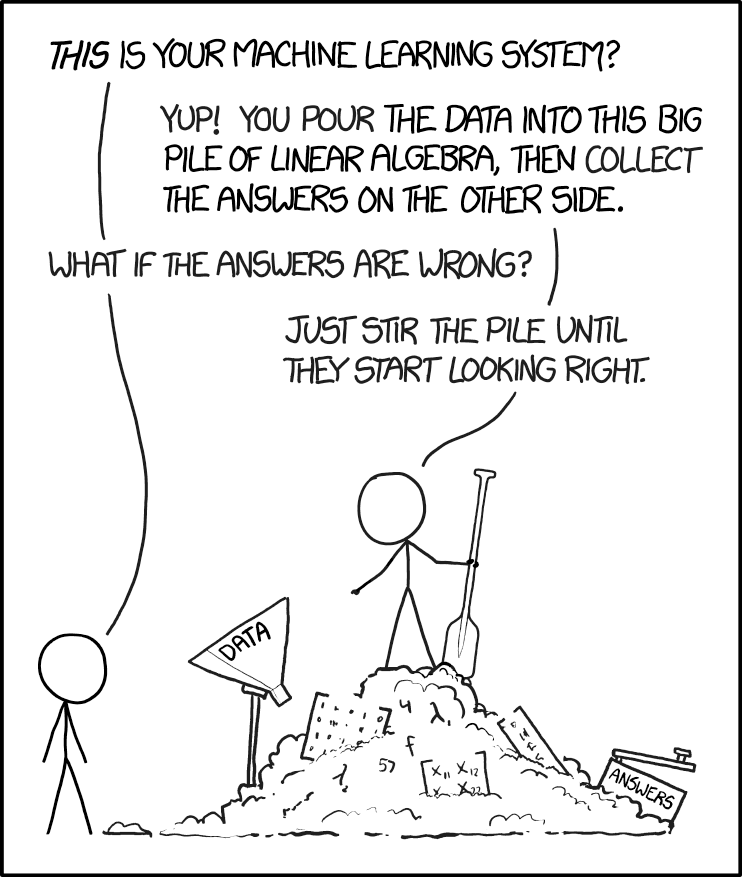
\includegraphics[width=0.5\textwidth]{machine_learning_2x.png}
		\vfill
		\large{Instituut voor Theoretische Fysica}\\
		\large{Faculteit der Natuurwetenschappen, Wiskunde en Informatica}\\
		\large{Universiteit van Amsterdam}\\~\\
		
\includegraphics[width=1.5cm]{UvA-logo.png}
	\end{center}
\end{titlepage}



\newpage
\thispagestyle{empty}

%%% NOTES
% \begin{itemize}
% \item The number of possible 1 ph-pair states increase with k up to a certain k and then saturates at a level of order $N$. For 2 ph-pairs it saturations at $N^3$.
% \item Better averaging state: high entropy state as averaging state because that makes the matrix element space flatter in sizes 
% \end{itemize}

\ 
\vfill
\noindent
\textbf{Cover image credit:} Randall Munroe, \textit{Machine Learning}, xkcd, \href{https://xkcd.com/1838/}{https://xkcd.com/1838/}.



\begin{savequote}[50mm]
Science is just magic that works.
\qauthor{Kurt Vonnegut, Cat's Cradle}
All sufficiently advanced technology is indistinguishable from magic.
\qauthor{Arthur C. Clark}
In the distance, the cat hears the sound of lobster minds singing in the void, a distant feed streaming from their cometary home as it drifts silently out through the asteroid belt, en route to a chilly encounter beyond Neptune. The lobsters sing of alienation and obsolescence, of intelligence too slow and tenuous to support the vicious pace of change that has sandblasted the human world until all the edges people cling to are jagged and brittle.
\qauthor{Charles Stross, Accelerando}
\end{savequote}
\chapter*{ }

% \epigraph{\textit{Science is just magic that works.}}{Kurt Vonnegut, Cat's Cradle}

% \epigraph{\textit{All sufficiently advanced technology is indistinguishable from magic.}}{Arthur C. Clark}



\tableofcontents

\newpage
\thispagestyle{plain}

\section*{Abstract}

Correlation functions play an important role in physics, but analytical results do not exist for many models.
For Bethe ansatz solvable models the ABACUS algorithm can be used to numerically find Fourier transformed correlation functions known as dynamical structure functions or DSFs.
This occurs through summing of matrix elements in the Lehmann series representation of the DSF.
This summing is not optimal, in that it does not sum matrix elements in strictly  monotonically decreasing order.

In this thesis we apply reinforcement learning to the summing of matrix elements, hoping to develop a strategy that leads to more optimal summation than done by ABACUS.
We develop a representation of the Lieb-Liniger model suitable for use in machine learning and use Q-learning to learn the summation strategy.
We find that the algorithm is able to learn to sum in such a way that it gives preference to highly contributing states, but that performance is far inferior to that shown by ABACUS.
As a corollary we also use supervised learning to try to optimize the numerical evaluation of Bethe ansatz parameters known as rapidities, but find that any advantage this method has declines considerably with system size.
The evaluation time added by the neural network makes this method unfit for finding rapidities.

\begin{savequote}[50mm]
The future is already here --- it's just not very evenly distributxed.
\qauthor{William Gibson}
\end{savequote}


\chapter{Introduction}

% \epigraph{\textit{The future is already here --- it's just not very evenly distributed.}}{William Gibson}

\noindent
Correlation functions are one of the central pillars of theoretical physics.
These functions, generally of the form
\begin{align}
  \label{eq:55}
  \expval{\mathcal{O}(x,t)\mathcal{O}(0,0)},
\end{align}
describe the correlations in time and space of microscopic variables.
Much work has been put in finding correlation functions for various models, but for many there is as yet no closed-form solution or this solution may not even exist.

In this thesis we consider the numerical evaluation of correlation functions for a class of models which are exactly solvable using the Bethe ansatz.
Solutions of Bethe ansatz solvable models take the form of (superpositions of) plane waves, parameterized by numbers known as rapidities.
If the system is quantized an equation known as the Bethe equation emerges, which allows for the calculation of these rapidities.
Many of the physical properties of Bethe ansatz solvable models can be expressed in terms of rapidities~\cite{Korepin1993}.
For this class of models the ABACUS algorithm~\cite{Caux2009} allows for the numerical evaluation of the Fourier transform of the correlation function, known as a dynamical structure function or DSF.

The DSF can be evaluated by considering its Lehmann series representation:
\begin{equation}\label{eq:lehmanintro}
  \mathcal{S}(k,\omega) = \frac{2\pi}{N}\sum_{\mu}\abs{\mel{\lambda^0}{\mathcal{O}_k}{\mu}}^2 \delta(\omega-E_{\mu}+E_0), 
\end{equation}
where the sum runs over the eigenstates of the model under consideration.
It is this summation on which we focus here.
The summing of the matrix elements in \cref{eq:lehmanintro} is difficult because the possible values of these matrix elements span many orders of magnitude.
To maximize efficiency in the calculation of DSFs it is thus desirable to start summing the largest matrix elements first and continue with progressively smaller values.
This ensures that the largest possible contributions to the DSFs are taken into account when a calculation reaches the maximum allowed computation time.
Ensuring this ordering of matrix elements is however a non-trivial task and ABACUS does not currently sum matrix elements in strictly monotonically decreasing order.
It is here that we may hope to see an improvement.

To that end we turn to reinforcement learning.
Reinforcement learning is a machine learning technique in which a computer learns a strategy for solving a problem by repeatedly trying different actions, observing the rewards these actions bring, and then altering it decision making process to optimize for higher rewards.
In the past five years reinforcement learning has seen a number of impressive results.
It has allowed superhuman performance on 1980s video games, purely by observing the pixels on screen~\cite{mnih13_playin_atari_with_deep_reinf_learn,mnih15_human_level_contr_throug_deep_reinf_learn}.
Much publicised was AlphaGo~\cite{silver16_master_game_go_with_deep}, a program capable of defeating the best human player in the board game Go, a feat that was thought to be at least a decade away.

While the initial version of AlphaGo first trained on human expert games and then went on to hone its abilities by playing itself, later versions started with only the rules of the game and learned purely by self-play~\cite{Silver2017a}.
This resulted in play that was stronger than when initially trained on human games, with the same result seen in chess and shogi (Chinese chess)~\cite{Silver2017}.
The Google Deepmind team behind these breakthroughs noted that~\cite{Silver2017a}, \textit{``Our results comprehensively demonstrate that a pure reinforcement learning approach is fully feasible, even in the most challenging of domains: it is possible to train to superhuman level, without human examples or guidance, given no knowledge of the domain beyond basic rules. Furthermore, a pure reinforcement learning approach requires just a few more hours to train, and achieves much better asymptotic performance, compared to training on human expert data.''}

It is this final quote which inspired the use of reinforcement learning in the domain of DSF calculation.
Our hope is that, given sufficient training, a reinforcement learning algorithm may beat the handcrafted heuristics used in ABACUS in efficiently summing matrix elements.
The main question we seek to answer in this thesis is whether we can train a reinforcement learning algorithm to do so.
To that end we must also determine which reinforcement learning algorithm is best suited for exploring the Hilbert space and how different states should be represented for use in a reinforcement learning environment.
As an addendum we will also consider whether the numerical calculation of rapidities benefits from using machine learning techniques.

This thesis is laid out as follows:
in \cref{chap:bethe_ansatz} we review some of the basics of the Bethe ansatz and its application in the Lieb-Liniger model, which we will use throughout this thesis because it has a number of properties that make it more simple to work with.
\Cref{chap:abacus} describes the ABACUS algorithm, its use, and the state scanning algorithm.
In \cref{chap:machine_learning} an introduction to machine learning and specifically reinforcement learning is given.
We describe our approach and results in \cref{chap:results}.
Finally \cref{chap:conclusion} discusses some of the difficulties inherent in reinforcement learning, summarizes our results and makes recommendations for future research directions.

\begin{sloppypar}
The code used to produce the results in this thesis may be found at \href{https://github.com/teunzwart/deepscanning}{https://github.com/teunzwart/deepscanning}.
\end{sloppypar}

\begin{savequote}[50mm]
You haff to vork very very hard.
\qauthor{Hans Bethe}
\end{savequote}

\chapter{The Bethe Ansatz}\label{chap:bethe_ansatz}

% \epigraph{\textit{You haff to vork very very hard.}}{Hans Bethe}

\noindent
The Bethe Ansatz allows for a way to solve certain one-dimensional systems exactly.
It was put forth by Bethe in 1931 to solve the Heisenberg model, refining and correcting the earlier work of Bloch~\cite{Bethe1931}.

\section{The Lieb-Liniger model}

Here, to introduce and understand the Bethe Ansatz, we focus on the Lieb-Liniger model, finding its eigenfunctions and excitation spectrum.
The Lieb-Liniger model, first introduced by Lieb and Liniger in 1963~\cite{Lieb1963, Lieb1963a}, consists of bosons interacting through a delta-function potential.
This model is described by the Hamiltonian
\begin{equation}
	H = - \sum_{j=1}^{N} \frac{\partial^2}{\partial x_j^2} + 2c \sum_{j<l} \delta(x_j - x_l).
\end{equation}
Here \(c\) is the interaction strength of the model, \(\hbar=1\) and we set \(2m=1\).
In the limit \(c\to0\) particles behave as free bosons, while \(c\to\infty\) yields fermionic behaviour and is known as the Tonks-Girardeau model~\cite{Lieb1963, Franchini2017}.
We will only solve the repulsive case (\(c > 0\)) here.

\subsection{A solution for the Schrödinger equation}

We will start solving the Lieb-Liniger model in the two-particle case, which readily generalizes to many particles.

For two particles, the Hamiltonian becomes
\begin{equation}
	H =  - \frac{\partial^2}{\partial x_1^2} - \frac{\partial^2}{\partial x_2^2} + 2c \delta(x_1 - x_2).
\end{equation}
We can write this in a more convenient form without the delta-function by integrating the Schrödinger equation over a small interval \([-\epsilon,\epsilon]\).
This yields the condition~\cite{Lieb1963} (see \cref{cha:boundary} for an explicit derivation)

\begin{equation}\label{eq:lieblinigerboundary}
	\left[\frac{\partial}{\partial x_2} - \frac{\partial}{\partial x_1} - c\right] \psi(x_1, x_2)\bigg\rvert_{x_1 = x_2} = 0.
\end{equation}
Since particles only interact with each other when their positions coincide, this allows us to simplify the Schrödinger equation to
\begin{equation}\label{eq:lieblinigersimple}
	\left[- \frac{\partial^2}{\partial x_1^2} - \frac{\partial^2}{\partial x_2^2}\right] \psi(x_1, x_2) = E \psi(x_1,x_2),
\end{equation}
with \cref{eq:lieblinigerboundary} as a boundary condition~\cite{Lieb1963}.
We assume an ordering of the positions \(x_1 < x_2\).
Since we are dealing with bosons, we also require the wave function to be symmetric: \(\psi(x_1,x_2) = \psi(x_2,x_1)\).
Effectively we have rewritten the Schrödinger equation such that we only consider the wave function away from the delta-function interaction points.
The boundary condition then reintroduces the interaction terms.

We can now conjecture a solution for the Lieb-Liniger model based on \cref{eq:lieblinigersimple}.
This equation can be solved in terms of a superposition of plane waves:
\begin{equation}
	\psi(x_1,x_2) = A_{12} e^{i(\lambda_1x_1 + \lambda_2 x_2)} + A_{21} e^{i(\lambda_2 x_1 + \lambda_1 x_2)},
\end{equation}
where the \(\lambda\)'s are pseudo-momenta, so-called because they are unobservable~\cite{Franchini2017}.
The \(A\)'s are the amplitudes of the plane waves making up the wave function.
Since \cref{eq:lieblinigerboundary} has to be fulfilled we require the amplitudes be related to each other by
\begin{align}
	\frac{A_{12}}{A_{21}} = -\frac{c-i(\lambda_1 - \lambda_2) }{c+i(\lambda_1 - \lambda_2)}.
\end{align}
The right-hand side of this equation has modulus 1, meaning it can be written as a phase:
\begin{align}
	\frac{A_{12}}{A_{21}} = -e^{i\phi(\lambda_1-\lambda_2)},
\end{align}
where~\cite{Korepin1993}
\begin{align}
  \phi(\lambda_1-\lambda_2) = i \log(\frac{\lambda_1-\lambda_2 + ic}{\lambda_1-\lambda_2-ic}),
\end{align}
or
\begin{align}
	\phi(\lambda_1-\lambda_2) = 2\arctan\left(\frac{\lambda_1-\lambda_2}{c}\right)
\end{align}
if we assume the argument of \(\phi\) to be real~\cite{Panfil2014}.

We can now write the two-particle wave function by setting \(A_{21}=1\) (and ignoring normalization for the moment) to get
\begin{equation}
	\psi(x_1,x_2) = - e^{-\frac{i}{2}\phi(\lambda_1-\lambda_2)+i(\lambda_1x_1 + \lambda_2 x_2)} + e^{\frac{i}{2}\phi(\lambda_1-\lambda_2)+i(\lambda_2 x_1 + \lambda_1 x_2)}.
\end{equation}
Generalization to the whole domain (not just where \(x_1 < x_2\)) can be achieved by requiring the wave function to be fully symmetric under coordinate exchange,
yielding
\begin{equation}
  \psi(x_1,x_2) = \textrm{sgn}(x_2-x_1)\sum_{P\in\pi_2} (-1)^{[P]} e^{i\lambda_{P_1}x_1 + i \lambda_2 x_2- \frac{i}{2} \textrm{sgn}(x_2-x_1)\phi(\lambda_{P_1}-\lambda_{P_2})}.
\end{equation}
The sum runs over the permutations of the set \((1,2)\)~\cite{Caux2015}.
This wave function is antisymmetric under exchange of quasimomenta, meaning that any wave function in which \(\lambda_1=\lambda_2\) is equal to 0.


Going to the many-particle state is now a fairly straightforward generalization of the two-particle case.
The wave function in this case becomes~\cite{Gaudin2009}
\begin{equation}
	\psi(x_1,\ldots,x_N) = \sum_{P\in\pi_N} A(P) e^{i\sum_j \lambda_{\mathcal{P}_j} x_j}
\end{equation}
where we sum over permutations of the set \((1,\ldots,N)\), and we have a condition on the amplitudes~\cite{Franchini2017}
\begin{align}
  \label{eq:41}
  \frac{A(\mathcal{P})}{A(\mathcal{P'})} = -e^{i\phi(\lambda_{\mathcal{P}} - \lambda_{\mathcal{P'}})}.
\end{align}


\subsection{Quantization}

Since we would like to study the properties of the system for finite densities, it is convenient to confine the system to a finite length \(L\).
This translates into a periodicity requirement for the wave function.
It require that the wave functions obeys~\cite{Franchini2017}
\begin{align}
	\psi(x_1,\ldots,x_j+L,\ldots,x_N) = \psi(x_1,\ldots,x_j,\ldots,x_N) \qquad \forall j\in 1,\ldots,N.
\end{align}
If we impose this condition on the wave function, the boundary term the quasimomenta have to obey the relation~\cite{Korepin1993}
\begin{equation}
  \label{eq:expbethe}
  e^{i\lambda_jL} = \prod_{l\neq j} \frac{\lambda_j-\lambda_l + ic}{\lambda_j - \lambda_l - ic}
\end{equation}
These are the Bethe equations.
If we take the logarithm of \cref{eq:expbethe} we get
\begin{align}
  \label{eq:bethe_equations}
  \lambda_j + \frac{1}{L} \sum_{l=1}^N \phi(\lambda_j - \lambda_l) = \frac{2\pi}{L}I_j, \qquad j = 1,\ldots,N,
\end{align}
where
\begin{align}
I_j \in 
\begin{cases}
  \mathbb{Z} + \frac{1}{2}, \qquad &N \textrm{ even}\\
  \mathbb{Z}  &N \textrm{ odd}
\end{cases}
\end{align}
The numbers \(I_j\) uniquely label the quasimomenta and are half-odd integers. 
They act as the quantum numbers of the theory.
These Bethe numbers may not coincide with each other, since this would also imply equal rapidities (\cref{th:equalisequal}).
Because the wave function is then equal to 0 such coincidences are not allowed, which is reminiscent of the Pauli principle~\cite{Caux2009,Franchini2017}.

We can get the momentum and energy of the Lieb-Liniger model from the rapidities. The momentum is given by summing over \cref{eq:bethe_equations}:
\begin{align}
  P = \sum_{j=1}^N \lambda_j = \frac{2\pi}{L}\sum_{j=1}^N I_j,
\end{align}
where the last step can be made because we sum the odd part of the Bethe equations over an even interval.
The energy meanwhile is~\cite{Korepin1993}
\begin{align}
  E = \sum_{j=1}^{N}\lambda_j^2.
\end{align}

The Bethe equations and Bethe numbers have a number of different properties:

\begin{theorem}\label{th:convexity}
\begin{sloppypar}
\noindent
The solutions of the Bethe equations \cref{eq:bethe_equations} are unique and exist, given a \mbox{(half-)integer} set of quantum numbers \(\{I\}\) \textup{\cite{Yang1969}}.
\end{sloppypar}
\end{theorem}
\begin{proof}
This can be proven with a variational argument, where the Bethe equations are the extremum of an action.
The Yang-Yang action for the Lieb-Liniger model is
\begin{align}
	S= \frac{L}{2} \sum_{j=1}^{N} \lambda_j^2 - 2\pi\sum_{j=1}^{N} n_j \lambda_j + \frac{1}{2} \sum_{j=1}^N \sum_{k=1}^{N} \theta_1(\lambda_j - \lambda_k),
\end{align}
where \(\theta_1(\lambda) = \int_0^{\lambda} \theta(\mu)\dd\mu\).
The Bethe equations follow from this by setting \(\frac{\partial S}{\partial \lambda_j} = 0\), which corresponds to a minimum.
To show this is indeed a minimum, we need to have a positive definite matrix of second derivatives:
\begin{align}
	\frac{\partial^2S}{\partial\lambda_j\partial\lambda_l} = \delta_{jl} \left[L + \sum_{m=1}^{N} \mathcal{C}(\lambda_j-\lambda_m)\right] - \mathcal{C}(\lambda_j- \lambda_l),
\end{align}
where we have the kernel
\begin{align}
	\mathcal{C}(\lambda - \mu) = \left.\frac{\dd \phi(x)}{\dd x} \right|_{x=\lambda-\mu} = \frac{2c}{c^2 + (\lambda - \mu)^2}.
\end{align}

By introducing a vector \(v_j\) with real components, we get~\cite{Korepin1993}
\begin{align}
  	\sum_{j,l}\frac{\partial^2S}{\partial\lambda_j\partial\lambda_l} v_jv_l = \sum_{j=1}^NL v_{j}^2 + \sum_{j>l=1}^{N} \mathcal{C}(\lambda_j-\lambda_m) (v_j - v_l)^2 \geq L \sum_{j=1}^Nv_j^{2} > 0,
\end{align}
meaning that the action is convex, and the minimum defining the Bethe equations is unique.
\end{proof}

\begin{theorem}
All solutions of the Bethe equations for the Lieb-Liniger model are real.
\end{theorem}

\begin{proof}
We consider the set of complex solutions to the Bethe equations \(\{\lambda_j\}\), where we call the value with the largest complex part in this set \(\lambda_{\max}\):
\begin{align}
\textrm{Im} \, \lambda_{\max} \geq \textrm{Im} \, \lambda_j.
\end{align}
If we put this into the non-logarithmic form of the Bethe equations and take the modulus we get
\begin{align}
  \left| e^{i\lambda_{\max} L} \right|= \left| \prod_k \frac{\lambda_{\max} - \lambda_k + ic}{\lambda_{\max} - \lambda_k - ic} \right|\geq 1,
\end{align}
since
\begin{align}
\left|\frac{\lambda+ic}{\lambda-ic} \right| \geq 1 \qquad \textrm{if Im}\, \lambda \geq 0.
\end{align}
This however means that \(\textrm{Im}\, \lambda_{\max} \leq 0\) since only then \(e^{i\lambda_{\max}L} \geq 1\).
Defining \(\textrm{Im}\,\lambda_{\min}\leq \lambda_j\) as the smallest imaginary part of a rapidity we can in the same way prove that \(\textrm{Im}\,\lambda_{\min} \geq 0\).
Taking these statements together we see that \(\textrm{Im}\, \lambda_{j}=0\textrm{\,}\forall\textrm{\,} j\), and hence all  \(\lambda\)'s are real~\cite{Korepin1993}.
\end{proof}

\begin{theorem}\label{th:equalisequal}
If \(I_j >I_k\), then \(\lambda_j > \lambda_k\). If \(I_j=I_k\) then \(\lambda_j=\lambda_k\).
\end{theorem}

\begin{proof}
Subtracting the relevant Bethe equations from each other we get
\begin{align}
  \lambda_j - \lambda_k + \frac{1}{L}\sum_{l=1}^N \left[\phi(\lambda_j - \lambda_l) - \phi(\lambda_k - \lambda_l)\right] = \frac{2\pi}{L} (I_j - I_k).
\end{align}
Because \(\abs{\atan(x)-\atan(y)}\leq\abs{x-y}\), the left side has the same sign as its first term, since the first term in the sum is larger than the second term, hence showing the theorem to be true~\cite{Korepin1993,Gaudin2009}.
\end{proof}



\subsection{Gaudin norm}
The norm of a Bethe eigenstate is given in terms of a determinant.
This result was first conjectured by Gaudin and for the Lieb-Liniger model takes the form~\cite{Caux2007}
\begin{align}
  \braket{\{\lambda\}}{\{\lambda\}} = c^N \prod_{k=1}^N \prod_{j=k+1}^N \frac{\lambda_{jk}^2 + c^2}{\lambda_{jk}} \det(\mathcal{G}(\{\lambda\})),
\end{align}
where $\mathcal{G}(\{\lambda\})$ is the Gaudin matrix of the state, with elements
\begin{align}\label{eq:gaudin}
  \mathcal{G}(\{\lambda\})_{jk} = \delta_{jk} \left(L + \sum_{m=1}^{N}\mathcal{C}(\lambda_j-\lambda_m)\right) - \mathcal{C}(\lambda_j, \lambda_k),
\end{align}
and \(\lambda_{jk} = \lambda_j-\lambda_k\).


\section{The thermodynamic limit}
\subsection{Ground state}
In going to the thermodynamic limit we let \(N\) and \(L\) tend to infinity, keeping \(D=N/L\) constant.
We first introduce a continuum version of the Bethe equations in terms of the function \(\lambda(x)\):
\begin{align}
  \label{eq:contbethe}
  L \lambda(x) + \sum_{k=1}^N\theta(\lambda(x)-\lambda_k) = 2 \pi L x.
\end{align}
where \(\lambda(x)\) takes values that are solutions to the original Bethe equations when \(x=I_j/L\): \(\lambda_j=\lambda(I_j/L)\).
If we invert the equation and take its derivative with respect to \(\lambda\) we get the density of particles in momentum space:
\begin{align}
  \rho(\lambda(x)) = \frac{\dd x(\lambda)}{\dd \lambda}.
\end{align}
This allows us to differentiate \cref{eq:contbethe} with respect to \(\lambda\) and write it as 
\begin{align}
  1+\frac{1}{L} \sum_{k=1}^{N} \mathcal{C}(\lambda(x)- \lambda_k) = 2\pi \rho(\lambda(x)).
\end{align}

If we now change the sum to an integral we get 
\begin{align}
  \frac{1}{L} \sum_l \mathcal{C}(\lambda(x)- \lambda_l) = \int_{-\lambda_F}^{\lambda_F} \mathcal{C}(\lambda,\mu) \rho(\mu) \dd \mu, 
\end{align}
leading to~\cite{Korepin1993}
\begin{align}
  \rho(\lambda) - \frac{1}{2\pi} \int_{-\lambda_F}^{\lambda^F} \mathcal{C}(\lambda-\mu) \rho(\mu) \dd \mu = \frac{1}{2\pi}.
\end{align}
This is the Lieb equation, which is the same as Love's equation in electrostatics, describing the capacitance of a circular capacitor~\cite{Gaudin2009}.
Together with 
\begin{align}
  D = \frac{N}{L} = \int_{-\lambda_F}^{\lambda_F} \rho(\lambda) \dd \lambda
\end{align}
this allows for the calculation of \(\rho(\lambda)\) for a given value of \(D\).


\subsection{Excitations}

Given the ground state we can build different excited states.
There are two types of excitations: particle-like (type I) excitations in which a new particle outside the Fermi interval is added with momentum \(k > \left|\lambda_F\right|\) and hole-like (type II) excitations, where a particle is removed from the Fermi interval with momentum \(k < \left|\lambda_F\right|\).
Additionally a particle may be excited out of the Fermi interval, but this is a combination of the other two excitations~\cite{Franchini2017}.

The \(N\)-particle ground state in terms of Bethe numbers is given by
\begin{align}
  \label{eq:22}
  \{I\} = \left\{-\frac{N-1}{2},-\frac{N-3}{2}, \ldots, \frac{N-3}{2},\frac{N-1}{2}\right\}.
\end{align}
Adding an excitation, changing the state to an \(N+1\)-particle state, results in
\begin{align}
  \label{eq:23}
    \{I\} = \left\{-\frac{N}{2},-\frac{N}{2}+1, \ldots, \frac{N}{2}-1,\frac{N}{2}+q\right\},
\end{align}
for \(q>0\).
Due to the coupled and non-linear nature of the Bethe equations, the addition of a single particle results in a change for all rapidities of the system~\cite{Franchini2017}.

We define the displacement of the rapidities as~\cite{Caux2015}
\begin{align}
  \label{eq:24}
  \frac{d_j}{L} = \lambda_j - \lambda_j^0,
\end{align}
with the superscript denoting that the rapidity is part of the ground state rapidity set.
Subtracting the Bethe equations of the ground state from the excited state we get~\cite{Franchini2017,Caux2015}
\begin{align}
  \label{eq:25}
   d_j = - \pi - \phi(\lambda_j-q) - \sum_{l=1}^{N} \left[\phi(\lambda_j - \lambda_l) - \phi(\lambda_j^0-\lambda_l^0)\right],
\end{align}
where \(q\) is the rapidity of the new particle.
Expanding the term in brackets gives\footnote{The expansions goes as follows:
  \begin{align*}
    \phi(\lambda_j-\lambda_l) - \phi(\lambda_j^0 - \lambda_l^0) &= \phi(\lambda_j^0 - \lambda_l^0 + \Delta\lambda) - \phi(\lambda_j^0 - \lambda_l^0) \quad \mathrm{where}\quad \Delta \lambda = \frac{1}{L}(d_j - d_l)\\
    &\approx\Delta \lambda \left.\frac{\partial\phi(x)}{\partial x} \right|_{x = \lambda_j^0-\lambda_l^0}
    = \frac{1}{L}(d_j-d_l) \frac{2c}{c^2 + (\lambda_j^0-\lambda_l^0)^2}.
  \end{align*}
}
\begin{align}
  \label{eq:27}
  d_j = -\pi - \phi(\lambda_j-q) - \frac{1}{L} \sum_{l=1}^N \frac{2c}{c^2 + (\lambda_j^0-\lambda_l^0)^2} (d_j-d_l) + \mathcal{O}\left(\frac{N}{L^2}\right),
\end{align}
or, by rearranging and turning the sums into integrals, extending \(d_j\to d(\lambda,q)\) to the continuum
\begin{multline}
  \label{eq:28}
  d(\lambda,q) \left(1+2\pi \int_{-\lambda_F}^{\lambda_F} \dd \lambda'\mathcal{C}(\lambda'-\lambda)\rho(\lambda')\right) = \\-\pi -\phi(\lambda-q) + 2\pi \int_{-\lambda_F}^{\lambda_F} \dd \lambda' \mathcal{C}(\lambda'-\lambda) \rho(\lambda') d(\lambda',q).
\end{multline}
If we use the Lieb equation and introduce \(D_p(\lambda,q)=d(\lambda,q)\rho(\lambda)\), which is the displacement function for particle-like excitations, we get the integral equation~\cite{Caux2015,Franchini2017}
\begin{align}
  \label{eq:partdisplacement}
  D_p(\lambda,q) - \int_{-\lambda_F}^{\lambda_F} \dd \lambda' \mathcal{C}(\lambda'-\lambda) D_p(\lambda', q) = \frac{-1}{2\pi} (\pi+\phi(\lambda-q)).
\end{align}

In dealing with holes we employ much the same ideas.
Starting from the \(N\)-particle ground state we can create a hole-like excitation by removing a particle in the Fermi interval to create an \(N-1\)-particle state with quantum numbers
\begin{align}
  \label{eq:26}
  \{I\} = \left\{-\frac{N}{2}+1,\ldots,\frac{N}{2}-m-1,\frac{N}{2}-m+1,\ldots,\frac{N}{2}\right\}.
\end{align}
Here \(0<m<\frac{N}{2}\) and we get a hole displacement function described by the integral equation~\cite{Caux2015}
\begin{align}
  \label{eq:holedisplacement}
  D_h(\lambda,q) - \int_{-\lambda_F}^{\lambda_F} \dd \lambda' \mathcal{C}(\lambda-\lambda') D_h(\lambda',q) = \frac{1}{2\pi}(\pi+\phi(\lambda-q)).
\end{align}






\section{Displacement functions for excitations}

From the previous section we have integral equations for the displacement functions of the Lieb-Liniger model.
We now turn to solving these equations.
To that end we introduce the truncated kernel:
\begin{align}
  \label{eq:inversetruncated}
  \mathcal{C}^{(F)}(\lambda,\lambda') = \theta(\lambda_F-\abs{\lambda}) \mathcal{C}(\lambda'-\lambda) \theta(\lambda_F-\abs{\lambda}).
\end{align}

Its associated inverse is defined by
\begin{align}
  \label{eq:32}
  	\left(1 + \mathcal{L}^{(F)}\right) * \left(1 - \mathcal{C}^{(F)}\right)(\lambda,\lambda')=\delta(\lambda-\lambda'), \quad \lambda, \lambda' \in \mathbb{R},
\end{align}
where we define \(*\) as the convolution:
\begin{align}
  \label{eq:29}
  (f*g)(x) = \int_{-\infty}^{\infty} \dd y f(x-y)g(y).
\end{align}
With this we can rewrite the differential equations for the displacement functions in \cref{eq:partdisplacement} and \cref{eq:holedisplacement} to be valid for a larger domain.

Using \cref{eq:inversetruncated} we can write the particle displacement integral equation as 
\begin{align}
  \label{eq:33}
  (1 - \mathcal{C}^{(F)}) * D_p(\lambda, \lambda_p) = -\frac{\theta(\lambda_F-\abs{\lambda})}{2\pi} (\pi\textrm{sgn}(\lambda_p)) + \phi(\lambda-\lambda_p))
\end{align}
for which the solution is 
\begin{align}
  \label{eq:34}
  D_p(\lambda,\lambda_p) = -\frac{1}{2\pi} \int_{-\lambda_F}^{\lambda_F} \dd \lambda' \left(\delta(\lambda-\lambda') + \mathcal{L}^{(F)}(\lambda,\lambda') \right)(\pi \mathrm{sgn}(\lambda_p) + \phi(\lambda'-\lambda_p)),
\end{align}
which is valid for all \(\abs{\lambda_p}>\lambda_F\) and all \(\lambda\).
We can use that
\begin{align}
  \label{eq:35}
  -\frac{1}{2\pi}(\pi \mathrm{sgn}(\lambda_p) + \phi(\lambda'-\lambda_p)) &= \frac{1}{2\pi} \int_{\lambda_p}^{\mathrm{sgn}(\lambda_p)\infty} \dd \lambda' \frac{\dd}{\dd\lambda'} \phi(\lambda-\lambda') \\
                                                                          &= - \int_{\lambda_p}^{\mathrm{sgn}(\lambda_p)\infty}\dd \lambda' \mathcal{C}(\lambda-\lambda'),
\end{align}
leading to~\cite{Caux2015}
\begin{align}
  \label{eq:particledisplacement}
  	D_p(\lambda, \lambda_p) = - \int_{\lambda_p}^{\textrm{sgn}(\lambda_p)\infty} \dd \lambda' \int_{-\lambda_F}^{\lambda_F} \dd  \lambda'' \left(\delta(\lambda-\lambda'') + \mathcal{L}^{(F)}(\lambda,\lambda'') \right)\mathcal{C}(\lambda''-\lambda').
\end{align}

For holes we have 
\begin{align}
  \label{eq:37}
  (1-\mathcal{C}^{(F)})* D_h(\lambda,\lambda_h) = \frac{\theta(\lambda_F-\abs{\lambda})}{2\pi} (\pi\mathrm{sgn}(\lambda_h) + \phi(\lambda-\lambda_F)),
\end{align}
for which the solution is 
\begin{align}
  \label{eq:38}
  D_h(\lambda,\lambda_h) = \frac{1}{2\pi} \int_{-\lambda_F}^{\lambda_F} \dd \lambda' \left(\delta(\lambda-\lambda')+\mathcal{L}^{(F)}(\lambda,\lambda')\right)(\pi\mathrm{sgn}(\lambda_h) + \phi(\lambda'-\lambda_h)).
\end{align}
Rewriting using
\begin{align}
  \label{eq:39}
  \frac{1}{2\pi} (\pi \mathrm{sgn}(\lambda_h) + \phi(\lambda-\lambda_h)) &= \frac{1}{2\pi} \int_{-\mathrm{sgn}(\lambda_h)\infty}^{\lambda_h} \dd \lambda' \frac{\dd}{\dd\lambda'} \phi(\lambda - \lambda') \\
                                                                         &= - \int_{-\mathrm{sgn}(\lambda_h)\infty}^{\lambda_h} \dd \lambda' \mathcal{C}(\lambda-\lambda')
\end{align}
gives
\begin{align}
  \label{eq:40}
  D_h(\lambda, \lambda_h) = - \int_{-\textrm{sgn}(\lambda_h)\infty}^{\lambda_h} \dd \lambda' \int_{-\lambda_F}^{\lambda_F} \dd \lambda'' \left(\delta(\lambda-\lambda'') + \mathcal{L}^{(F)}(\lambda,\lambda'') \right)\mathcal{C}(\lambda''-\lambda'),
\end{align}
which is valid for all \(\abs{\lambda_h}<\lambda_F\) and all \(\lambda\)~\cite{Caux2015}.

We now simplify the displacement functions for particle-like (type I) and hole-like (type~II) excitations, first for the ground state and then for excited states.
Note that the expression we find differ from those in e.g.~\cite{Korepin1993}, because they assume that in the displacement functions \(\mathcal{L}^{F}\) inverts \(\mathcal{C}\), which is not the case.

\subsection{The ground state}
\begin{sloppypar}
For type I excitations we have the displacement function \cref{eq:particledisplacement}.
We can rewrite this in a more explicit way.
Lets first focus on the part involving the \(\delta\)-function, which we can rewrite, using a Heaviside step function, as
\begin{align}
	- \int_{\lambda_p}^{\textrm{sgn}(\lambda_p)\infty} &\dd \lambda' \int_{-\lambda_F}^{\lambda_F} \dd  \lambda'' \delta(\lambda-\lambda'') \mathcal{C}(\lambda''-\lambda') \\
	&=- \int_{\lambda_p}^{\textrm{sgn}(\lambda_p)\infty} \dd \lambda' \int_{-\infty}^{\infty} \dd \lambda'' \theta(\lambda_F - \abs{\lambda''})  \delta(\lambda-\lambda'') \mathcal{C}(\lambda''-\lambda')\\
	&= - \theta(\lambda_F - \abs{\lambda}) \int_{\lambda_p}^{\textrm{sgn}(\lambda_p)\infty} \dd \lambda'     \mathcal{C}(\lambda-\lambda').
\end{align}
We change variables \(a=\lambda-\lambda'\):
\begin{equation}\label{eq:integratedkerneldeltapart}
	- \theta(\lambda_F - \abs{\lambda}) \int_{\lambda_p}^{\textrm{sgn}(\lambda_p)\infty} \dd \lambda'     \mathcal{C}(\lambda-\lambda')=
	 \theta(\lambda_F - \abs{\lambda}) \int_{\lambda-\lambda_p}^{\lambda - \textrm{sgn}(\lambda_p)\infty} \dd a\,\mathcal{C}(a).
\end{equation}
Assuming \(\lambda\) to be finite, the upper bound of the integral reduces to \(-\textrm{sgn}(\lambda_p)\infty\).
\end{sloppypar}

\Cref{eq:integratedkerneldeltapart} is 0 if \(\abs{\lambda} > \lambda_F\), so the only \(\lambda\)'s we have to consider in the integral are \(\abs{\lambda}< \lambda_F\), but from the definition of the displacement we know \(\abs{\lambda_p}  >\lambda_F\), meaning \(\abs{\lambda_p} > \abs{\lambda}\) for all \(\lambda\) in the integral.
Therefore \(\lambda-\lambda_p\) always has the opposite sign from~\(\lambda_p\).
Thus we can rewrite \cref{eq:integratedkerneldeltapart} as
\begin{align}
	\theta(\lambda_F - \abs{\lambda}) \int_{\lambda-\lambda_p}^{\lambda - \textrm{sgn}(\lambda_p)\infty} \dd a\,\mathcal{C}(a) &=
	\theta(\lambda_F - \abs{\lambda}) \int_{-\textrm{sgn}(\lambda_p)\abs{\lambda-\lambda_p}}^{ - \textrm{sgn}(\lambda_p)\infty} \dd a\,\mathcal{C}(a).
\end{align}

Since the kernel is symmetric,  the value of the integral does not depend on whether \(\mathrm{sgn}(\lambda_p)\) is \(+1\) or \(-1\).
This only adds a sign-function in front of the integral:
\begin{align}
	\theta(\lambda_F - \abs{\lambda}) \int_{-\textrm{sgn}(\lambda_p)\abs{\lambda-\lambda_p}}^{ - \textrm{sgn}(\lambda_p)\infty} \dd a\,\mathcal{C}(a) &= - \textrm{sgn}(\lambda_p) \theta(\lambda_F - \abs{\lambda}) \int_{\abs{\lambda-\lambda_p}}^{\infty} \dd a\,\mathcal{C}(a)\\
	&= - \frac{1}{2\pi} \textrm{sgn}(\lambda_p) \theta(\lambda_F - \abs{\lambda})  \left( \pi - 2\atan(\frac{\abs{\lambda - \lambda_p}}{c})\right)\label{eq:dpdeltanonsimplified}\\
	&= - \frac{1}{\pi} \textrm{sgn}(\lambda_p) \theta(\lambda_F - \abs{\lambda})  \atan\left(\frac{c}{\abs{\lambda-\lambda_p}}\right),
\end{align}
where the last equality is valid because the argument of the arctangent is strictly positive.
It is important to remark that the above expression would not be valid without the Heaviside function, since the integral may only be solved in the manner above when \(\abs{\lambda}< \lambda_F\).

The second part of \cref{eq:particledisplacement}, which involves \(\mathcal{L}^{(F)}(\lambda,\lambda')\), can't be rewritten in closed form, since there is no closed form solution for \(\mathcal{L}^{(F)}(\lambda,\lambda')\).
We can however rewrite this term to get rid of the improper integral, which will help in numerical evaluation of the expression.
We have
\begin{align}
	- \int_{\lambda_p}^{\textrm{sgn}(\lambda_p)\infty} &\dd \lambda' \int_{-\lambda_F}^{\lambda_F} \dd \lambda''  \mathcal{L}^{(F)}(\lambda,\lambda'') \mathcal{C}(\lambda''-\lambda')\\
	&= -  \int_{-\lambda_F}^{\lambda_F} \dd \lambda''   \mathcal{L}^{(F)}(\lambda,\lambda'') \left[\int_{\lambda_p}^{\textrm{sgn}(\lambda_p)\infty} \dd \lambda'\mathcal{C}(\lambda''-\lambda') \right]\\
	&=   \int_{-\lambda_F}^{\lambda_F} \dd \lambda''   \mathcal{L}^{(F)}(\lambda,\lambda'') \left[\int_{\lambda''-\lambda_p}^{\lambda''-\textrm{sgn}(\lambda_p)\infty} \dd a\,\mathcal{C}(a) \right]\\
	&= -\textrm{sgn}(\lambda_p) \int_{-\lambda_F}^{\lambda_F} \dd \lambda''   \mathcal{L}^{(F)}(\lambda,\lambda'') \left[\int_{\abs{\lambda''-\lambda_p}}^{\infty} \dd a\,\mathcal{C}(a) \right]\\
	&= -\frac{1}{\pi}\textrm{sgn}(\lambda_p) \int_{-\lambda_F}^{\lambda_F} \dd \lambda''   \mathcal{L}^{(F)}(\lambda,\lambda'') \left[\frac{\pi}{2} - \atan(\frac{\abs{\lambda''-\lambda_p}}{c})\right]\\
	&= -\frac{1}{\pi}\textrm{sgn}(\lambda_p) \int_{-\lambda_F}^{\lambda_F} \dd \lambda''   \mathcal{L}^{(F)}(\lambda,\lambda'') \atan(\frac{c}{\abs{\lambda''-\lambda_p}}),
\end{align}
where, as before, we argued that \(\abs{\lambda''} < \abs{\lambda_p}\) and thus that \(\lambda'' - \lambda_p\) always has the opposite sign from \(\lambda_p\).

Taking these results together, the displacement function for type I excitations becomes 
\begin{multline}
	D_p(\lambda, \lambda_p) = - \frac{1}{\pi} \textrm{sgn}(\lambda_p) \theta(\lambda_F - \abs{\lambda})  \atan\left(\frac{c}{\abs{\lambda-\lambda_p}}\right) \\-\frac{1}{\pi}\textrm{sgn}(\lambda_p) \int_{-\lambda_F}^{\lambda_F} \dd \lambda''   \mathcal{L}^{(F)}(\lambda,\lambda'') \atan(\frac{c}{\abs{\lambda''-\lambda_p}}).
\end{multline}
An example is plotted in \cref{fig:dpplot}.
\begin{figure}[tb!]
  \centering
  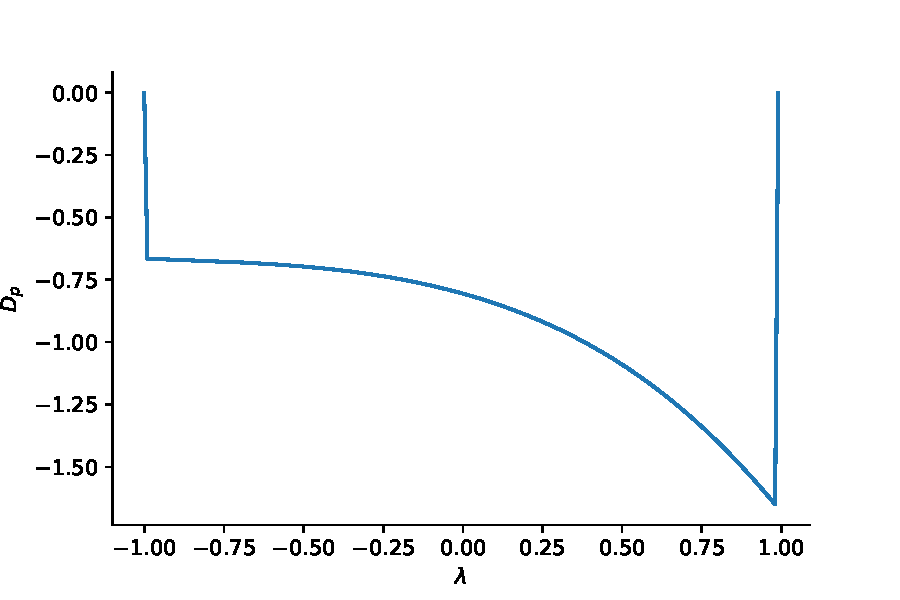
\includegraphics[width=0.7\textwidth]{dpplot.pdf}
  \caption{$D_p(\lambda,\lambda_p)$ plotted for \(c=1\), \(\lambda_F=1\), \(\lambda_p=1.5\).}
  \label{fig:dpplot}
\end{figure}

For type II excitations the idea is much the same as type I. Recalling \cref{eq:40}, the displacement is
\begin{equation}
	D_h(\lambda, \lambda_h) = - \int_{-\textrm{sgn}(\lambda_h)\infty}^{\lambda_h} \dd \lambda' \int_{-\lambda_F}^{\lambda_F} \dd \lambda'' \left(\delta(\lambda-\lambda'') + \mathcal{L}^{(F)}(\lambda,\lambda'') \right)\mathcal{C}(\lambda''-\lambda'),
\end{equation}
which is valid for all \(\lambda_h\) (if \(\abs{\lambda_h} < \lambda_F\)) and all \(\lambda\)~\cite{Caux2015}.
The \(\delta\)-function part of this equation becomes
\begin{align}
	-\int_{-\textrm{sgn}(\lambda_h)\infty}^{\lambda_h} \dd \lambda' \int_{-\lambda_F}^{\lambda_F} \dd \lambda'' \delta(\lambda-\lambda'') \mathcal{C}(\lambda''-\lambda') 
		= - \theta(\lambda_F - \abs{\lambda}) \int_{-\textrm{sgn}(\lambda_h)\infty}^{\lambda_h} \dd \lambda'     \mathcal{C}(\lambda-\lambda').
\end{align}
A change of variables \(a=\lambda-\lambda'\) results in:
\begin{align}
	 - \theta(\lambda_F - \abs{\lambda}) \int_{-\textrm{sgn}(\lambda_h)\infty}^{\lambda_h} \dd \lambda'     \mathcal{C}(\lambda-\lambda') = 
	  \theta(\lambda_F - \abs{\lambda}) \int_{\lambda+\textrm{sgn}(\lambda_h)\infty}^{\lambda-\lambda_h} \dd a \, \mathcal{C}(a).
\end{align}
Since we again assume \(\lambda\) to be finite, the lower bound of the integral reduces to \(\textrm{sgn}(\lambda_h)\infty\).
Because both \({\abs{\lambda_h} < \lambda_F}\) and \({\abs{\lambda} < \lambda_F}\) (due to the Heaviside function), we can no longer make statements about the sign of \(\lambda-\lambda_h\) and have to be a bit more general in our expression.
We get
\begin{align}
	  \theta(\lambda_F - \abs{\lambda}) \int_{\textrm{sgn}(\lambda_h)\infty}^{\lambda-\lambda_h} \dd a \, \mathcal{C}(a) 
	  &= \frac{1}{\pi}\theta(\lambda_F - \abs{\lambda}) \left[ \atan(\frac{\lambda-\lambda_h}{c}) - \textrm{sgn}(\lambda_h)\frac{\pi}{2}\right].
\end{align}

For hole-like excitations, the part of the displacement function involving \(\mathcal{L}^{(F)}(\lambda,\lambda')\) becomes
\begin{align}
	 - \int_{-\textrm{sgn}(\lambda_h)\infty}^{\lambda_h} &\dd \lambda' \int_{-\lambda_F}^{\lambda_F} \dd \lambda''  \mathcal{L}^{(F)}(\lambda,\lambda'') \mathcal{C}(\lambda''-\lambda')\\
	 &= - \int_{-\lambda_F}^{\lambda_F} \dd \lambda''  \mathcal{L}^{(F)}(\lambda,\lambda'')\left[ \int_{-\textrm{sgn}(\lambda_h)\infty}^{\lambda_h} \dd \lambda' \mathcal{C}(\lambda''-\lambda')\right]\\
	 &= \int_{-\lambda_F}^{\lambda_F} \dd \lambda''  \mathcal{L}^{(F)}(\lambda,\lambda'')\left[ \int_{\textrm{sgn}(\lambda_h)\infty}^{\lambda''-\lambda_h} \dd a \, \mathcal{C}(a)\right]\\
	 &= \frac{1}{\pi}\int_{-\lambda_F}^{\lambda_F} \dd  \lambda''  \mathcal{L}^{(F)}(\lambda,\lambda'')\left[ \atan(\frac{\lambda''-\lambda_h}{c}) - \textrm{sgn}(\lambda_h)\frac{\pi}{2}\right],
\end{align}
assuming \(\lambda''\) finite.

The expression for the displacement of type II excitations is thus
\begin{multline}
	D_h(\lambda, \lambda_h) = \frac{1}{\pi}\theta(\lambda_F - \abs{\lambda}) \left[ \atan(\frac{\lambda-\lambda_h}{c}) - \textrm{sgn}(\lambda_h)\frac{\pi}{2}\right] \\+
	\frac{1}{\pi}\int_{-\lambda_F}^{\lambda_F} \dd  \lambda''  \mathcal{L}^{(F)}(\lambda,\lambda'')\left[ \atan(\frac{\lambda''-\lambda_h}{c}) - \textrm{sgn}(\lambda_h)\frac{\pi}{2}\right],
\end{multline}
with an example plotted in \cref{fig:dhplot}.
\begin{figure}[tb!]
  \centering
  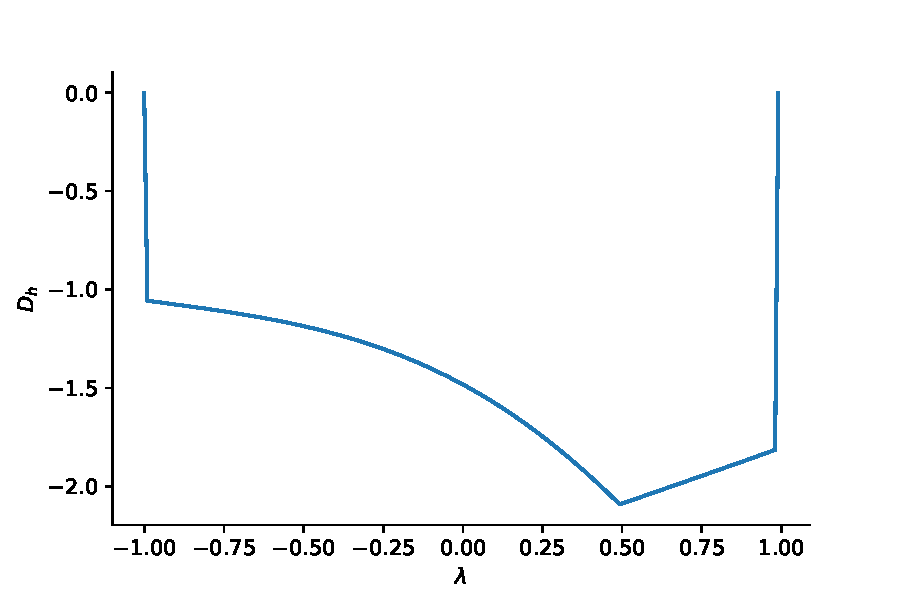
\includegraphics[width=0.7\textwidth]{dhplot.pdf}
  \caption{$D_h(\lambda,\lambda_h)$ plotted for \(c=1\), \(\lambda_F=1\), \(\lambda_h=0.5\).}
  \label{fig:dhplot}
\end{figure}

\subsection{Calculating \(\mathcal{L}^{(F)}\)}

In the above expressions we still have \(\mathcal{L}^{(F)}\), for which there is no closed form solution, and which thus has to be numerically evaluated.

Recalling \cref{eq:32}, the definition of \(\mathcal{L}^{(F)}\) is~\cite{Caux2015}
\begin{equation}
	\left(1 + \mathcal{L}^{(F)}\right) * \left(1 - \mathcal{C}^{(F)}\right)(\lambda,\lambda')=\delta(\lambda-\lambda'), \quad \lambda, \lambda' \in \mathbb{R}
\end{equation}
or explicitly
\begin{equation}
	\int_{-\infty}^{\infty} \dd \lambda'' \left( \delta(\lambda-\lambda'') + \mathcal{L}^{(F)}(\lambda,\lambda'')\right)\left(\delta(\lambda''-\lambda') - \mathcal{C}^{(F)}(\lambda'',\lambda')\right) = \delta(\lambda-\lambda'),
\end{equation}
with  \(\lambda, \lambda', \lambda'' \in \mathbb{R}\).
If we perform the integration, cancel common terms and rearrange, we get the integral equation
\begin{align}
	\mathcal{L}^{(F)}(\lambda,\lambda') &= \int_{-\infty}^{\infty} \mathcal{L}^{(F)}(\lambda,\lambda'') \mathcal{C}^{(F)}(\lambda'',\lambda') + \mathcal{C}^{(F)}(\lambda,\lambda')\\
	&= \theta(\lambda_F - \abs{\lambda'}) \int_{-\lambda_F}^{\lambda_F} \dd \lambda'' \mathcal{L}^{(F)}(\lambda,\lambda'') \mathcal{C}(\lambda''-\lambda') + \mathcal{C}^{(F)}(\lambda,\lambda')
\end{align}

So far we have been exact.
Now we can make use of the method of successive approximation~\cite{Zemyan2012} to solve this equation (a Fredholm integral equation of the second kind).

If we have an integral equation of the form
\begin{equation}
  \phi(x) = f(x) + \omega \int_{a}^b K(x,t)\phi(t) \dd t,
\end{equation}
where $K(x,t)$ is a continuous integration kernel on the interval $[a,b]$, then it seems reasonable to assume that to lowest order the solution of the integral equation is $f(x)$, provided that $\omega$ is small.
This gives a lowest order approximation $\phi_0(x) = f(x)$, subsequent substitution yielding 
\begin{equation}
  \phi(x) = f(x) + \omega \int_{a}^b K(x,t)\phi_0(t) \dd t,
\end{equation}
which we hope to be more tractable than the original equation.
In general the $n+1$-th approximation is defined in terms of the $n$-th approximation as
\begin{equation}
  \phi_{n+1}(x) = f(x) + \omega \int_{a}^b K(x,t)\phi_n(t) \dd t.
\end{equation}
This converges as long as $\abs{\omega} \lVert K \rVert_2 < 1$, with $\lVert K \rVert_2$ the $L_2$-norm:
\begin{equation}
  \lVert K \rVert_2 = \left( \int_{a}^b \int_a^b \abs{K(x,t)}^2 \dd x \dd t\right)^{1/2}.
\end{equation}

For the case we are interested in we have 
\begin{equation}
  \mathcal{L}^{(F)}_{n+1} (\lambda, \lambda') = \theta(\lambda_F - \abs{\lambda'}) \int_{-\lambda_F}^{\lambda_F} \mathcal{L}^{(F)}_n(\lambda, \lambda'') \mathcal{C} (\lambda''-\lambda') \dd \lambda'' + \mathcal{C}^{(F)}(\lambda, \lambda'),
\end{equation}
which converges as long as 
\begin{equation}
\left(\frac{2\lambda_F}{\pi^2c^3} \atan(\frac{2\lambda_F}{c})\right)^{1/2} < 1.
\end{equation}
If we only wish to know the value of $\mathcal{L}^{(F)}$ at a single point we can
use that at each iteration step $\mathcal{L}^{(F)}$ is simply a number, allowing us to take it out of the integral.
We get
\begin{gather}
  \mathcal{L}^{(F)}_{n+1} (\lambda, \lambda') = \theta(\lambda_F - \abs{\lambda'})  \mathcal{L}^{(F)}_n(\lambda, \lambda') \int_{-\lambda_F}^{\lambda_F} \mathcal{C} (\lambda''-\lambda') \dd \lambda'' + \mathcal{C}^{(F)}(\lambda, \lambda')\\
= - \frac{1}{\pi} \theta(\lambda_F - \abs{\lambda'}) \mathcal{L}^{(F)}_n(\lambda, \lambda') \left[ \atan(\frac{\lambda'+\lambda_F}{c}) - \atan(\frac{\lambda'-\lambda_F}{c})\right] + \mathcal{C}^{F}(\lambda,\lambda'),
\end{gather}
where \(\mathcal{L}^{(F)}_0(\lambda, \lambda')\) is 0. An example of a numerical evaluation of \(\mathcal{L}^{(F)}\) is seen in \cref{fig:lfplot}.
\begin{figure}[tb!]
  \centering
  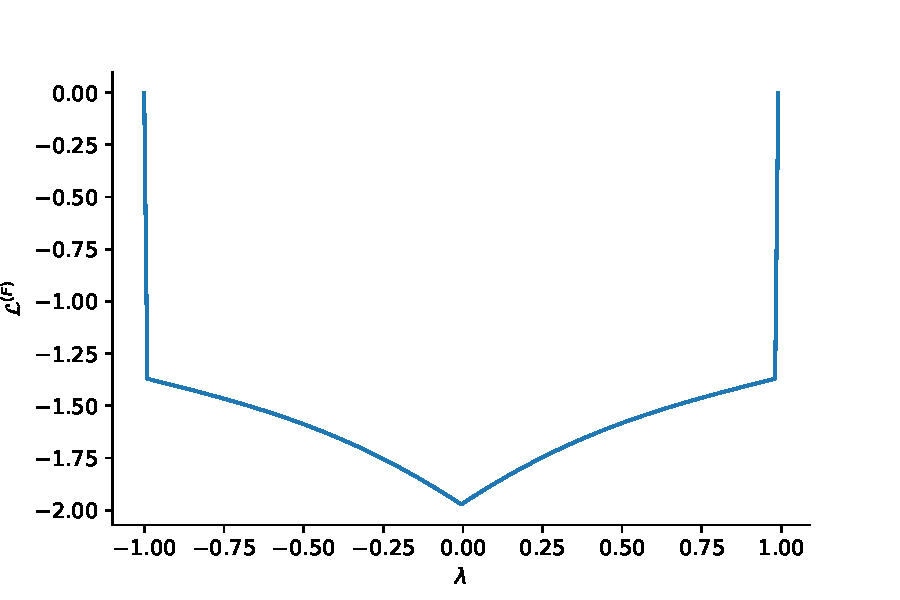
\includegraphics[width=0.7\textwidth]{lfplot.pdf}
  \caption{\(\mathcal{L}^{(F)}(\lambda,\lambda')\) plotted for \(c=1\), \(\lambda_F = 1\), \(\lambda'=0\).}
  \label{fig:lfplot}
\end{figure}

\subsection{Excited states}

For excited states there is no longer a Fermi level~\cite{Caux2015} (or the Fermi level goes to \(\infty\)), meaning that the truncated kernel \(\mathcal{C}^{(F)}\) becomes equal to the regular Lieb-Liniger kernel~\(\mathcal{C}\).
The displacement function for type I and II excitations are respectively~\cite{Caux2015}
\begin{align}
	D_p(\lambda, \lambda_p) = - \int_{\lambda_p}^{\textrm{sgn}(\lambda_p)\infty} \dd \lambda' \int_{-\infty}^{\infty} \dd  \lambda'' \left[\delta(\lambda-\lambda'') + \mathcal{L}(\lambda-\lambda'') \right]\mathcal{C}(\lambda''-\lambda'),
\end{align}
and
\begin{align}
	D_h(\lambda, \lambda_h) = - \int_{-\textrm{sgn}(\lambda_h)\infty}^{\lambda_h} \dd \lambda' \int_{-\infty}^{\infty} \dd \lambda'' \left[\delta(\lambda-\lambda'') + \mathcal{L}(\lambda - \lambda'') \right]\mathcal{C}(\lambda''-\lambda'),
\end{align}
where \(\mathcal{L}\) is the inverse of of the kernel \(\mathcal{C}\), defined by~\cite{Yang1969}
\begin{align}
	(1+\mathcal{L})*(1-\mathcal{C})(\lambda) = \delta(\lambda),
\end{align}
or explicitly
\begin{align}
	\int_{-\infty}^{\infty} \dd \lambda' \left[ \delta(\lambda-\lambda') + \mathcal{L}(\lambda-\lambda') \right] \left[ \delta(\lambda') - \mathcal{C}(\lambda')\right] = \delta(\lambda), \quad \lambda, \lambda' \in \mathbb{R}.
\end{align}
If we perform the integral and rearrange, we get an expression which simplifies the displacement functions:
\begin{align}\label{eq:kernelinversion}
	\int_{-\infty}^{\infty} \dd \lambda' \mathcal{L}(\lambda-\lambda') \mathcal{C}(\lambda') = -\mathcal{C}(\lambda) + \mathcal{L}(\lambda).
\end{align}

With this in hand, we have for particles:
\begin{align}
	D_p(\lambda, \lambda_p) &= - \int_{\lambda_p}^{\textrm{sgn}(\lambda_p)\infty} \dd \lambda' \int_{-\infty}^{\infty} \dd  \lambda'' \left[\delta(\lambda-\lambda'') + \mathcal{L}(\lambda-\lambda'') \right]\mathcal{C}(\lambda''-\lambda')\\
	&= - \int_{\lambda_p}^{\textrm{sgn}(\lambda_p)\infty} \dd \lambda' \left[\mathcal{C}(\lambda-\lambda') + \int_{-\infty}^{\infty} \dd  \lambda'' \mathcal{L}(\lambda-\lambda'') \mathcal{C}(\lambda''-\lambda')\right]\\
	&= - \int_{\lambda_p}^{\textrm{sgn}(\lambda_p)\infty} \dd \lambda' \left[\mathcal{C}(\lambda-\lambda') - \mathcal{C}(\lambda-\lambda') + \mathcal{L}(\lambda-\lambda')\right]\\
	&= - \int_{\lambda_p}^{\textrm{sgn}(\lambda_p)\infty} \dd \lambda' \mathcal{L}(\lambda-\lambda')\\
	&=  \int_{\lambda-\lambda_p}^{-\textrm{sgn}(\lambda_p)\infty} \dd a \, \mathcal{L}(a),
\end{align}
where we used \cref{eq:kernelinversion} in going from the second to the third line, and made the substitution \(a = \lambda-\lambda'\) in the last line.
A very similar derivation for type II excitations leads to
\begin{align}
	D_h(\lambda,\lambda_h) = \int_{\textrm{sgn}(\lambda_h)\infty}^{\lambda-\lambda_h} \dd a\, \mathcal{L}(a).
\end{align}


\section{Form factors}
As a final part of this chapter, we look at form factors for the Lieb-Liniger model, which we will require for calculation of dynamical structure functions (see \cref{chap:abacus}).
Form factors or matrix elements may be obtained by using the algebraic Bethe ansatz (until now we used a coordinate representation of the wave function known as the coordinate Bethe ansatz).
We will briefly introduce the algebraic Bethe ansatz. 

\subsection{The algebraic Bethe ansatz}

In the algebraic Bethe ansatz (ABA) we define our operators in terms of fields.
The quantized Hamiltonian of the Lieb-Liniger model is\footnote{The derivation of this is found in~\cite{feynman}.}
\begin{align}
  \label{eq:30}
  H = \int_0^L \dd x \left(\partial_x \Psi^{\dag}(x) \partial_x \Psi(x) + c \Psi^{\dag}(x)\Psi^{\dag}(x)\Psi(x)\Psi(x)\right),
\end{align}
with the field operators obeying the commutation relation \([\Psi^{\dag}(x),\Psi(y)] = \delta(x-y)\).

In the ABA a fundamental object is the monodromy matrix, consisting of operators \(A(\lambda), B(\lambda), C(\lambda), D(\lambda)\):
\begin{align}
  \label{eq:31}
  T(\lambda) =
  \begin{pmatrix}
    A(\lambda) & B(\lambda) \\
    C(\lambda) & D(\lambda)
  \end{pmatrix},
\end{align}
where 
\begin{align}
  \label{eq:36}
  A(\lambda) \ket{0} = a(\lambda)\ket{0},\qquad D(\lambda) \ket{0} = d(\lambda)\ket{0},
\end{align}
when acting on the vacuum \(\ket{0}\).
Physical states may be build using \(B(\lambda)\) and \(C(\lambda)\):
\begin{align}
  \label{eq:42}
  \ket{\{\lambda\}} = \prod_{j=1}^{N} B(\lambda_j) \ket{0} \quad \mathrm{and} \quad \bra{\{\lambda\}} = \bra{0} \prod_{j=1}^N C(\lambda_j).
\end{align}
In the Lieb-Liniger model~\cite{Piroli2015}
\begin{align}
  \label{eq:43}
  a(\lambda) = e^{-i\frac{L}{2}\lambda}, \qquad d(\lambda) = e^{i\frac{L}{2}\lambda}.
\end{align}

The commutation relations between the operators are encoded in the Yang-Baxter equation~\cite{Korepin1993}, which depend on an object known as the \(R\)-matrix.
In the case of the Lieb-Liniger model, the \(R\)-matrix is
\begin{align}
  \label{eq:45}
  R(\lambda,\mu) = 
  \begin{pmatrix}
    f(\lambda, \mu) & 0 & 0 & 0\\
    0 & g(\lambda, \mu) & 1 & 0\\
    0 & 1 & g(\lambda, \mu) & 0 \\
    0 & 0 & 0 & f(\lambda,\mu)
  \end{pmatrix},
\end{align}
with
\begin{align}
  \label{eq:46}
  f(\lambda,\mu) = \frac{\lambda-\mu+ic}{\lambda-\mu}, \qquad g(\lambda,\mu) = \frac{ic}{\lambda-\mu}.
\end{align}

To explicitly determine the action on states of the field operator, in terms of which physical operators are defined, we use the commutation relations
\begin{align}
  \label{eq:47}
  [\Psi(0),B(\lambda)] = -i \sqrt{c} A(\lambda), \qquad [C(\lambda), \Psi^{\dag}(0)] = i \sqrt{c} D(\lambda).
\end{align}
This allows us to derive
\begin{align}
  \label{eq:48}
  \Psi(0) \prod_{k=1}^N B(\lambda_k) \ket{0} &= -i\sqrt{c} \sum_{k=1}^N\Lambda_k a(\lambda_k) \prod_{\substack{m=1\\m\neq k}}^N B(\lambda_m) \ket{0},\\
  \bra{0} \prod_{k=1}^N C(\lambda_k) \Psi^{\dag}(0) &= i \sqrt{c} \sum_{k=1}^N \bra{0} \prod_{\substack{m=1\\m\neq k}}^N C(\lambda_m) \widetilde{\Lambda} d(\lambda_k),
\end{align}
with~\cite{Piroli2015}
\begin{align}
  \label{eq:49}
  \Lambda_k = \prod_{\substack{m=1\\m\neq k}}^N f(\lambda_k,\lambda_m), \qquad \widetilde{\Lambda}_k = \prod_{\substack{m=1\\m\neq k}}^N f(\lambda_m,\lambda_k).
\end{align}

With these tools, form factors of operators may be calculated.
We have only skimmed the surface of the ABA.
A (much) more thorough introduction may be found in~\cite{Korepin1993} and~\cite{slavnov18_algeb_bethe_ansat}.


\subsection{Form factor for \(\rho\) operator}

Now we can calculate the form factor of the density operator.
We only present here the result, referring to~\cite{slavnov90_noneq_time_curren_correl_funct} for the derivation.

The density operator is~\cite{Nardis2015}
\begin{align}
  \hat{\rho}(x) = \sum_{j=1}^N \delta(x-x_j),
\end{align}
with \(\{x_j\}_{j=1}^N\) the positions of the particles in the gas, or in terms of fields~\cite{slavnov90_noneq_time_curren_correl_funct}
\begin{align}
  \label{eq:44}
  \hat{\rho}(x) = \Psi^{\dag}(x)\Psi(x).
\end{align}
The form factor is~\cite{slavnov90_noneq_time_curren_correl_funct, Nardis2015}
\begin{multline}
  \label{eq:rho_form_factor}
  \matrixel{\{\mu\}}{\hat{\rho}(0)}{\{\lambda\}} = \frac{\det(I_N +U)}{V^+(p) - V^-(p)}
  \left(\sum_{j=1}^N(\mu_j-\lambda_j)\right) \times\\ \prod_{j=1}^N\left(V^+(\lambda_j) - V^-(\lambda_j)\right)\prod_{j=1}^N\prod_{k=1}^N\left(\frac{\lambda_j-\lambda_k+ic}{\mu_j-\lambda_k}\right),
\end{multline}
with element of the matrix \(U\) given by
\begin{align}
  U_{jk} = i \frac{\mu_j-\lambda_j}{V^+(\lambda_j) -V^-(\lambda_j)}\prod_{\substack{m=1\\m\neq j}}^N \left(\frac{\mu_m - \lambda_j}{\lambda_m-\lambda_j}\right) \left(K(\lambda_j, \lambda_k) - K(p, \lambda_k)\right),
\end{align}
and 
\begin{align}
  \label{eq:56}
  V(\lambda_j)^{\pm} = \prod_{k=1}^N \frac{\mu_k-\lambda_j\pm ic}{\lambda_k-\lambda_j\pm ic}.
\end{align}
The parameter \(p\) is an arbitrary complex numbers which is not necessarily in the set of rapidities of the states.
We will generally set it to zero, since that simplifies numerical evaluation of \cref{eq:rho_form_factor} and the form factor does not depend on their values.
Note that for the Lieb-Liniger model \(V(\lambda_j)^{-} = (V(\lambda_j)^{+})^{*}\), since all rapidities are real in this case.

Including normalization we have for the form factors \(\mathcal{F}\)~\cite{Nardis2015}
\begin{align}
  \label{eq:21}
  \mathcal{F}(\{\mu\}, \{\lambda\}) = \frac{\matrixel{\{\mu\}}{\hat{\rho}(x)}{\{\lambda\}}}{\sqrt{\innerproduct{\{\mu\}}{\{\mu\}}\innerproduct{\{\lambda\}}{\{\lambda\}}}}.
\end{align}
If two states have the same momentum, the matrix element vanishes~\cite{slavnov90_noneq_time_curren_correl_funct}, while if $\{\mu\} = \{\lambda\}$ we have $\mathcal{F}=\frac{N}{L}$.

\begin{savequote}[50mm]
Hilbert space is a big place.
\qauthor{Unknown}
\end{savequote}


\chapter{The ABACUS algorithm}\label{chap:abacus}

% \epigraph{\textit{Hilbert space is a big place.}}{Unknown}

\noindent
The ABACUS algorithm, developed by Caux et al.~\cite{Caux2005, Caux2007, Caux2007a, Caux2005a}, allows for the computation of dynamical correlation functions.
Despite some analytic progress~\cite{Nardis2016,Nardis2015,slavnov90_noneq_time_curren_correl_funct}, this is still mostly a numerical affair.

Specifically we are interested in calculating two-point zero-temperature equilibrium\footnote{At the time of writing ABACUS is also capable of calculating correlation function at arbitrary temperature and out-of-equilibrium (having been developed further since the appearance of~\cite{Caux2009} in 2009), but we will not consider that here further.} correlation functions of the form
\begin{equation}\label{eq:expval}
	\expval{\mathcal{O}_j(t)\mathcal{O}_{j'}^{\dagger}(0)},
\end{equation}
where \(j=1\ldots N\) denotes lattice sites.
This is the expectation value for arbitrary time separations $t$ and distances $j-j'$.
The equivalent Fourier transformed quantity is the dynamical structure factor (DSF)
\begin{equation}\label{eq:DSF}
	\mathcal{S}(k,\omega) = \frac{1}{N} \sum_{j,j'=1}^{N} \exp^{-ik(j-j')} \int_{-\infty}^{\infty}\dd t \exp^{i\omega t}\expval{\mathcal{O}_j(t)\mathcal{O}_{j'}^{\dagger}(0)}.
\end{equation}
We can construct \cref{eq:expval} from this given knowledge of the DSF for all energies and momenta, but \cref{eq:DSF} is often more useful because it is the quantity directly accessible in experiments~\cite{Caux2009,Caux2007a}.

Calculating \cref{eq:DSF} is often still complicated, but by introducing the Fourier transform of the operators $\mathcal{O}_k=\sum_j \exp^{-ikj} \mathcal{O}_j$, and performing the time integrations, we get the Lehmann series representation of the DSF:
\begin{equation}
  \label{eq:lehman}
  \mathcal{S}(k,\omega) = \frac{2\pi}{N}\sum_{\mu}\abs{\mel{\lambda^0}{\mathcal{O}_k}{\mu}}^2 \delta(\omega-E_{\mu}+E_0), 
\end{equation}
where we sum over intermediate eigenstates of the Hamiltonian under consideration, with $E_0$ the energy of the ground state $\ket{\lambda^0}$.
The matrix elements $\mel{\lambda}{\mathcal{O}}{\mu}$ are known as form factors.

In order to calculate DSFs we require
\begin{itemize}
  \item an orthonormal eigenstate basis
  \item form factors for the operator $\mathcal{O}_k$ we are interested in
  \item a way to do the summation over the intermediate states
\end{itemize}
The first and second item are provided by the Bethe ansatz.
The summation proves to be more difficult, but for this we can use ABACUS (Algebraic Bethe Ansatz-based Computation of Universal Structure factors) to perform it numerically.
As long as a system is Bethe ansatz integrable and finite in size ABACUS can in principle compute its DSF.
Even for large systems the results are highly accurate, with this accuracy being mostly energy and momentum independent~\cite{Caux2009}.
In fact, the accuracy can be measured using sum rules, and saturation in excess of 99\% is possible for systems with hundreds of particles.


\section{Numerically solving the Bethe equations}\label{sec:numer-solv-bethe}

In general the computation of rapidities of Bethe integrable systems is a complex affair, with complex rapidities making the computation difficult.
For the Lieb-Liniger model however there is a simplifying condition, since the rapidities are all real and the Yang-Yang system of the model is convex (see \cref{th:convexity}), meaning there is a unique solution for a given set of quantum numbers.

In this case we can use the matrix Newton method to calculate rapidities.
To introduce this method we first look at the one-dimensional case.
If we want to find the value of \(x\) that solves \(f(x)=0\), we can iteratively approximate this value by 
\begin{equation}
  x^{k+1} = x^k - \frac{f(x^k)}{f'(x^k)}, \qquad k = 0, 1, 2, \ldots,
\end{equation}
with given starting value \(x_0\).
This converges quadratically (meaning on each iteration \(k+1\) the error \(\epsilon_{k+1}\) is of order \(\epsilon_k^2\)).

Now we can turn to the case at hand, where we solve the Bethe equations.
These are coupled non-linear equations of the general form \(\mathbf{f(x)=0}\).
In this case we can find the solution \(x\) by iteratively applying the formula
\begin{equation}
  \mathbf{x}^{k+1} = \mathbf{x}^k - {[J(\mathbf{x}^k)]}^{-1}\mathbf{f}(\mathbf{x}^k), \qquad k=0,1,2\ldots,
\end{equation}
where \(J\) is the Jacobian matrix of \(\mathbf{f}\) and \(\mathbf{x}_0 \in \mathbb{R}^n\).
Just as in the single variable case this converges quadratically.

To prevent the calculation of the inverse of the Jacobian, in practice Newton's method is used in the form
\begin{equation}\label{eq:practicalnewton}
  J(\mathbf{x}^k)[\mathbf{x}^{k+1} - \mathbf{x}^k] = - \mathbf{f}(\mathbf{x}^k),
\end{equation}
where, given \(\mathbf{x}^k\), we calculate \(J(\mathbf{x}^k)\) and \( \mathbf{f}(\mathbf{x}^k)\), and then solve the system of linear coupled equations to obtain \(\Delta\mathbf{x}=\mathbf{x}^{k+1} - \mathbf{x}^k\), which is added to \(\mathbf{x}^k\) to obtain \(\mathbf{x}^{k+1}\)~\cite{Sueli2003}. 
This linear system can be solved using LU decomposition~\cite{Press2007}.\footnote{In an LU decomposition we can rewrite the set of linear equations:
  \begin{align}
    \label{eq:54}
    \mathbf{A}\cdot\mathbf{x} = (\mathbf{L}\cdot\mathbf{U}) \cdot \mathbf{x} =\mathbf{L}\cdot(\mathbf{U}) \cdot \mathbf{x}) = \mathbf{b},
  \end{align}
decomposing \(\mathbf{L}\cdot\mathbf{U} = \mathbf{A}\) in a lower and an upper triangular matrix.
The advantage of this is that we can now solve this system in two parts, first solving \(\mathbf{L}\cdot\mathbf{y} = \mathbf{b}\), and then solving \(\mathbf{U}\cdot\mathbf{x} = \mathbf{y}\), which is easier to do with a triangular matrix~\cite{Press2007}.
}

In ABACUS we are of course interested in the Bethe equations.
Here we will specifically look at those of the Lieb-Liniger model.
Recalling \cref{chap:bethe_ansatz}, the Bethe equations in logarithmic form are 
\begin{align}
  \lambda_j + \frac{1}{L} \sum_{l=1}^N \phi(\lambda_j - \lambda_l) = \frac{2\pi}{L}I_j, \qquad j = 1,\ldots,N,
\end{align}
or
\begin{align}
  \frac{2\pi}{L}I_j - \lambda_j + \frac{1}{L} \sum_{l=1}^N \phi(\lambda_j - \lambda_l) = B(\{\lambda\}),
\end{align}
with
\begin{equation}
  \phi(\lambda_j - \lambda_l) = -2\arctan\left(\frac{\lambda_j-\lambda_l}{c}\right).
\end{equation}

If we recast this is the shape of \cref{eq:practicalnewton}, we get
\begin{equation}
  \mathcal{G}(\{\lambda^k\}) \Delta \lambda = -B(\{\lambda^k\}),
\end{equation}
where we used that the Jacobian of the Bethe equations is equal to the Gaudin matrix (\cref{eq:gaudin})~\cite{Caux2009}.

Additionally, damping may be employed while solving the system, with the updating of \(\lambda\) looking like
\begin{align}
  \label{eq:dampednewton}
  \lambda^{k+1} = \lambda^k + \gamma \Delta \lambda.
\end{align}
Defining the difference squared as
\begin{align}
  \label{eq:51}
  \Delta^2 = \frac{1}{N}\sum_{i=1}^{N} \left(\frac{\Delta \lambda_i}{\lambda_i}\right)^2,
\end{align}
the update algorithm for \(\gamma\) at each iteration is
\begin{algorithm}
  \begin{algorithmic}[0]
    \If{$\Delta^2_{k+1} > \Delta_{k}^2$ \textbf{and} $\gamma_k >0.5$} 
    \State{$\gamma_{k+1} = 0.5 \gamma_{k}$}
    \ElsIf{$\Delta^2_{k+1} < \Delta_{k}^2$} 
    \State{$\gamma_{k+1} = 1$}
    \Else{}
    \State{$\gamma_{k+1} = \gamma_k$}
    \EndIf{}
  \end{algorithmic}
\end{algorithm}

The Bethe equations for real rapidities are considered solved when~\cite{Caux2009}
\begin{equation}
	\Delta^2 < 10^4 \times \epsilon^2,
\end{equation}
where \(\epsilon\) is machine precision for the datatype double, which is ``the difference between 1 and the least value greater than 1 that is representable''~\cite{cppstandard2016}.
On machines implementing IEEE 754-2008 (the standard for floating-point arithmetic)~\cite{ieeefp2008} this is equal to \({2^{-52} \approx 2.22 \times 10^{-16}}\).


\section{Scanning over the Hilbert space}

With the rapidities in hand (and the form factors and Gaudin norm readily computed therefrom, see~\cref{chap:bethe_ansatz}), we are now faced with the summation over states.
At face value we may now hit a wall, since we are tasked with exploring a factorially large space and find eigenstates with monotonically decreasing absolute numerical form factor values.
The dimensionality of the state space is equal to the number of allowable choices of quantum numbers because a Pauli-like principle is at work.
For the Lieb-Liniger model (where all rapidities are real, and for a particle preserving operator), given $M$ particles and a UV cutoff for the upper, respectively lower bound of the quantum number $I_{\infty+}$, $I_{\infty-}$, the number of states is~\cite{Caux2009}\footnote{This is the number of states if particle Bethe numbers can not exceed the UV-cutoffs. In the current implementation of ABACUS scanning within a single momentum slice is possible, which may include states in which individual particles exceed \(I_{\max}\), but which sum to lie within the allowed interval. Therefore this number may now be seen as a lower limit on the size of the Hilbert space under consideration.}
\begin{equation}
  \binom{I_{\infty+} + I_{\infty-} + 1}{M} = \frac{(I_{\infty+} + I_{\infty-} + 1)!}{M!(I_{\infty+} + I_{\infty-} + 1 - M)!}.
\end{equation}
Luckily, there are some principles that allow for the definition of an efficient algorithm for scanning the Hilbert space.

First, form factors for large enough systems are approximately continuous, meaning the changing of a single quantum number does not change the form factor a lot.
Therefore, given an eigenstate with a large form factor and thus a large contribution to the DSF, we can scan states close to this given state to find other large contributions.

Second, form factors between the ground state and excited states generally decrease when more particle-hole excitations are created in the area in pseudo-momentum space clamped by the Fermi level.

Third, as quantum numbers become larger, moving further from the Fermi level in quantum number space, the form factors also decrease~\cite{Caux2009}.

With these principles we can start to define a way for scanning the Hilbert space.
Starting from the lowest-energy state we generate states with low-lying particle-hole pair excitations in the Fermi interval (low-lying meaning they are close to the center of the interval).
If the contributions from these states to the chosen sum rule are large enough, further scanning of this state commences, with increasing complexity of the state in the form of more particle-hole pairs.

Large enough, in the context above, means that the form factor associated with the state is above the so-called \textit{running threshold}, with initial value such that the number of intermediate states is of order \(N^2\).
The form factors are kept, and the threshold is lowered after a scan and a new scan is initiated of those sectors in the Hilbert space for which the average form factor is above the current running threshold.
ABACUS thus keeps track of the already scanned states in the Hilbert space to allow knowledge to be gathered on where to scan next as well as to avoid doubly counting states~\cite{Caux2009}.

In practice we are therefore descending a ``mountain'' of form factors as slowly as possible, always trying to move in the direction of smallest change.
This proves especially difficult since the form factors are not monotonically decreasing while moving around in Hilbert space.
ABACUS can not fully compensate for this non-monotonicity, as is seen in \cref{fig:orderedmagnitudes}, where the absolute magnitude of form factors is plotted as a function of their order in the computation.
We see both that some highly contributing form factors are missed early on, appearing as spikes in the distribution later, as well as see small form factors spuriously being considered early, resulting in wasted computations.
\begin{figure}[tb!]
  \centering
  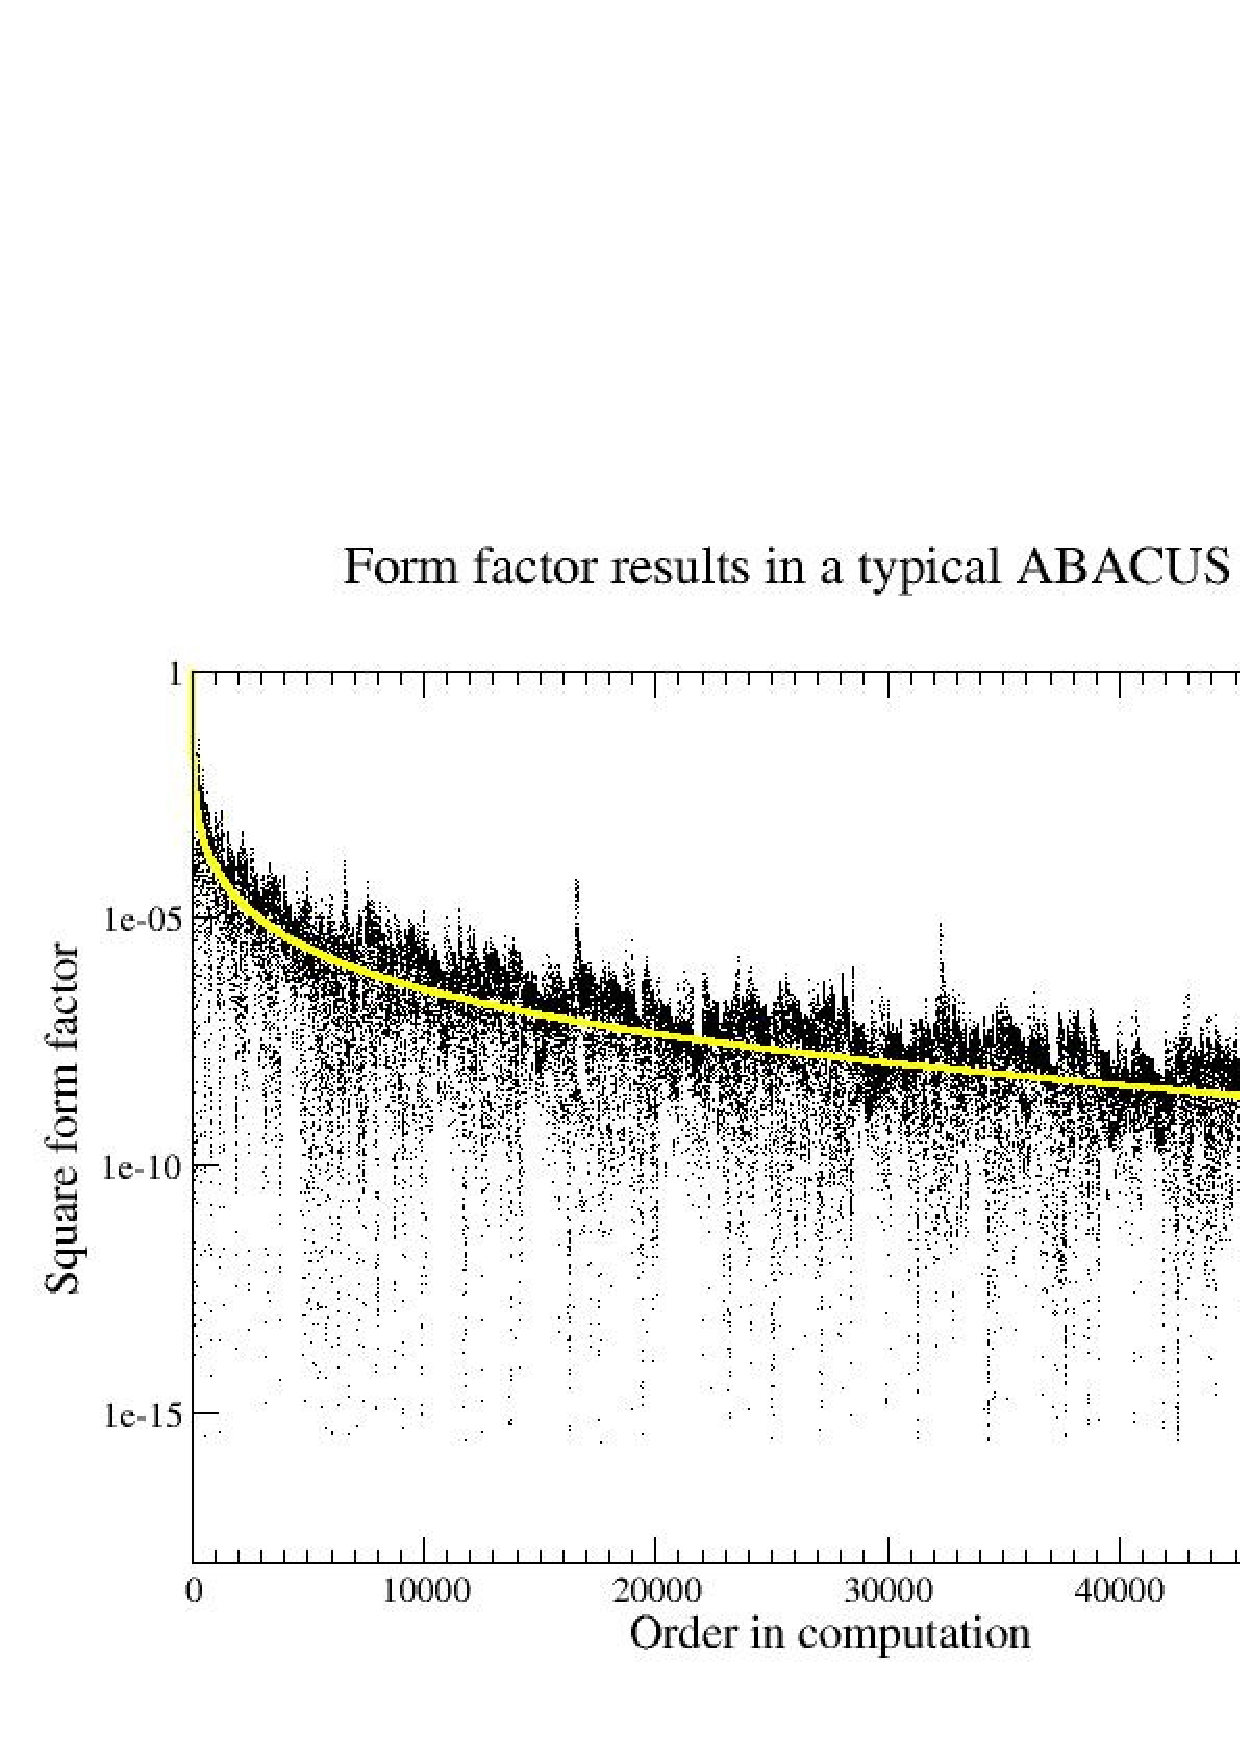
\includegraphics[width=\textwidth]{FFsq_vs_order_D0p6N50M20_small}
  \caption{Size of matrix element magnitudes encountered while summing intermediate states of the XXZ model. The yellow line denotes strictly decreasing magnitude. Note that while in general the size of the form factors decreases, not all large form factors are immediately found. Figure taken from~\cite{Caux2009}.}
\label{fig:orderedmagnitudes}
\end{figure}

After an ABACUS run, the available data consists of a set of energy-momentum-form factor triplets.
The quality of this data, in terms of how well it captures important contributions from the Hilbert space, can be determined with sum rules.
A suitable candidate of these is the f-sum rule~\cite{Caux2007a}, which relates the first energy moment over the DSF to a function of \(k\).
With this sum rule the intensity in individual momentum slices can be explicitly determined.
For the density-density correlation function of the Lieb-Liniger model this becomes
\begin{align}
  \label{eq:fsumrule}
  \int_{-\infty}^{\infty} \frac{\dd \omega}{2\pi} \omega \mathcal{S}(k, \omega) = \frac{1}{N}\sum_{\mu}(E_{\mu}-E_0)\abs{\mel{\lambda^0}{\rho}{\mu}}^2  = \frac{N}{L} k^2.
\end{align}
A full derivation of the generic formula, as well as the specific case above may be found in~\cref{cha:f-sum-rule}. 

\Cref{fig:lieb_density_dsf} shows the DSF in energy-momentum space for the density-density correlator of the Lieb-Liniger model obtained from ABACUS runs.
In \cref{table:saturation} the efficiency of ABACUS is showcased.
It presents the number of states necessary to reach a given saturation in the XXZ model\footnote{The XXZ model is another Bethe ansatz integrable model consisting of spins with Hamiltonian~\cite{Franchini2017}
    \begin{align}
      \label{eq:53}
      H = - J \sum_{n=1}^N\left[S_{n}^xS_{n+1}^x+S_n^yS_{n+1}^y + \Delta S_n^zS_{n+1}^z\right].
    \end{align}
} and the fraction of the Hilbert space necessary to reach this saturation.
Although the algorithm is not perfect, only very small fractions are necessary.

\begin{figure}[tb!]
  \centering
  \begin{tabular}{cc}
    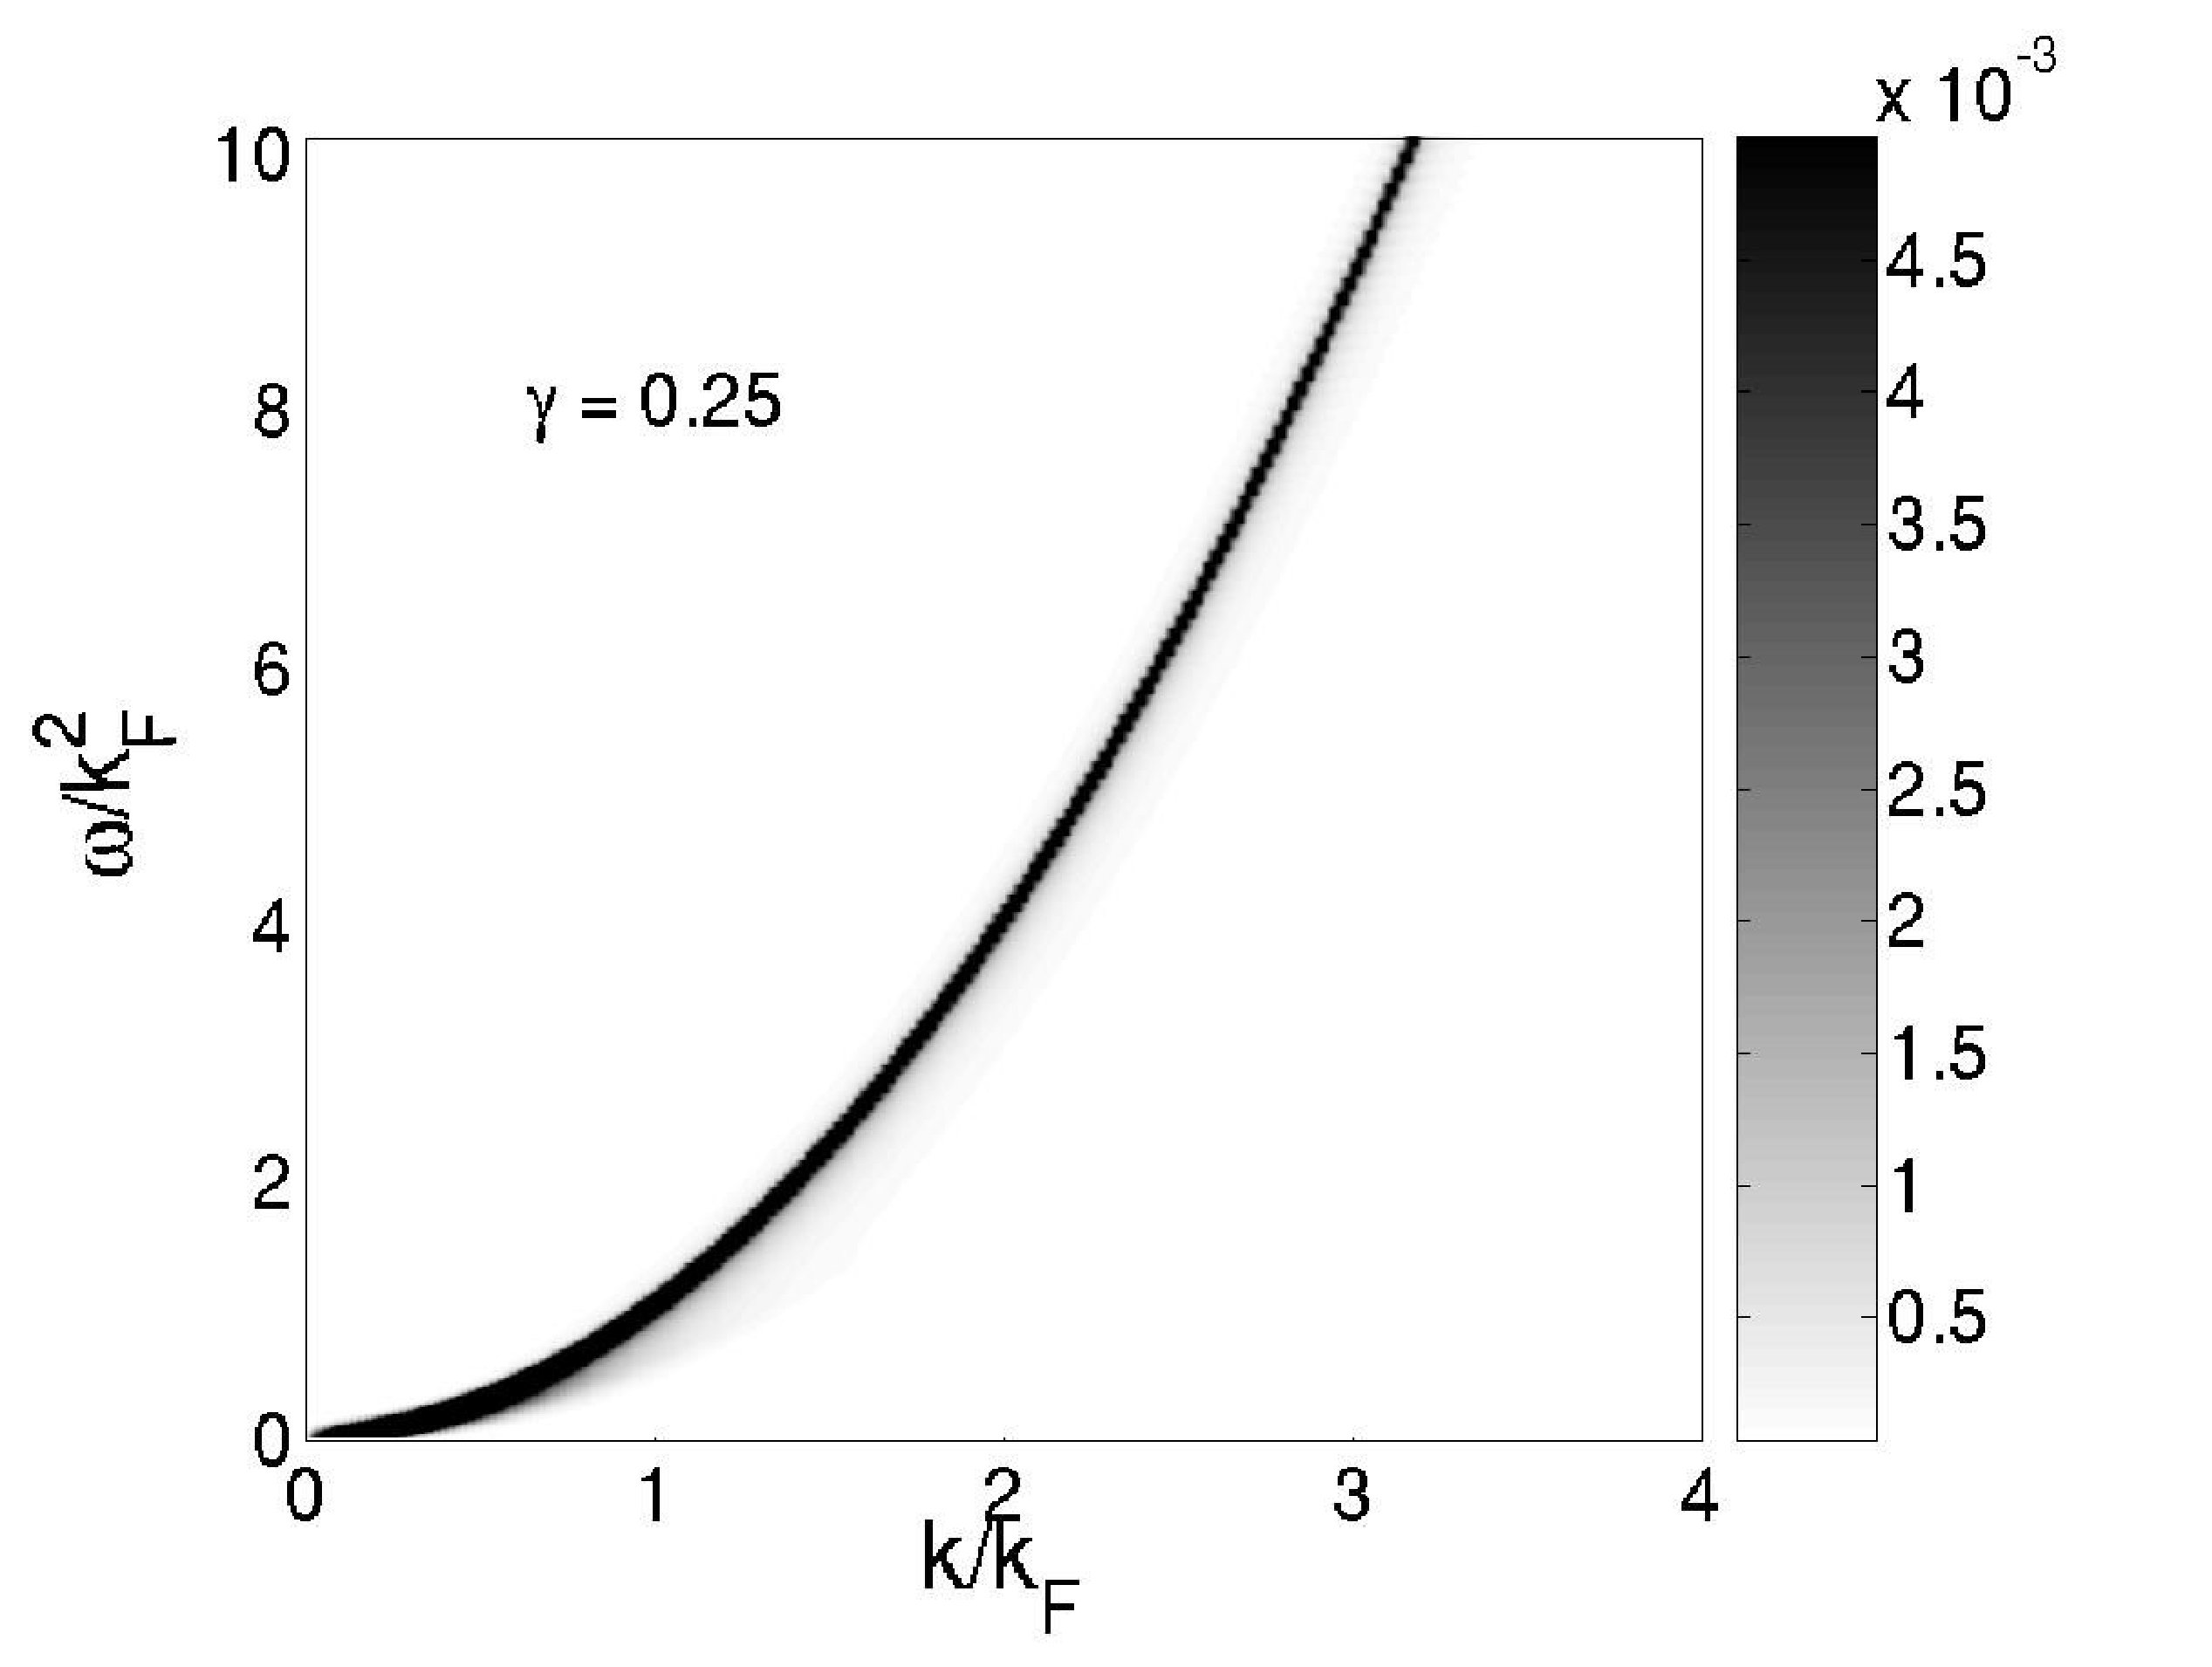
\includegraphics[width=4.3cm]{c_0p25_L_100_N_100.eps}
    &
      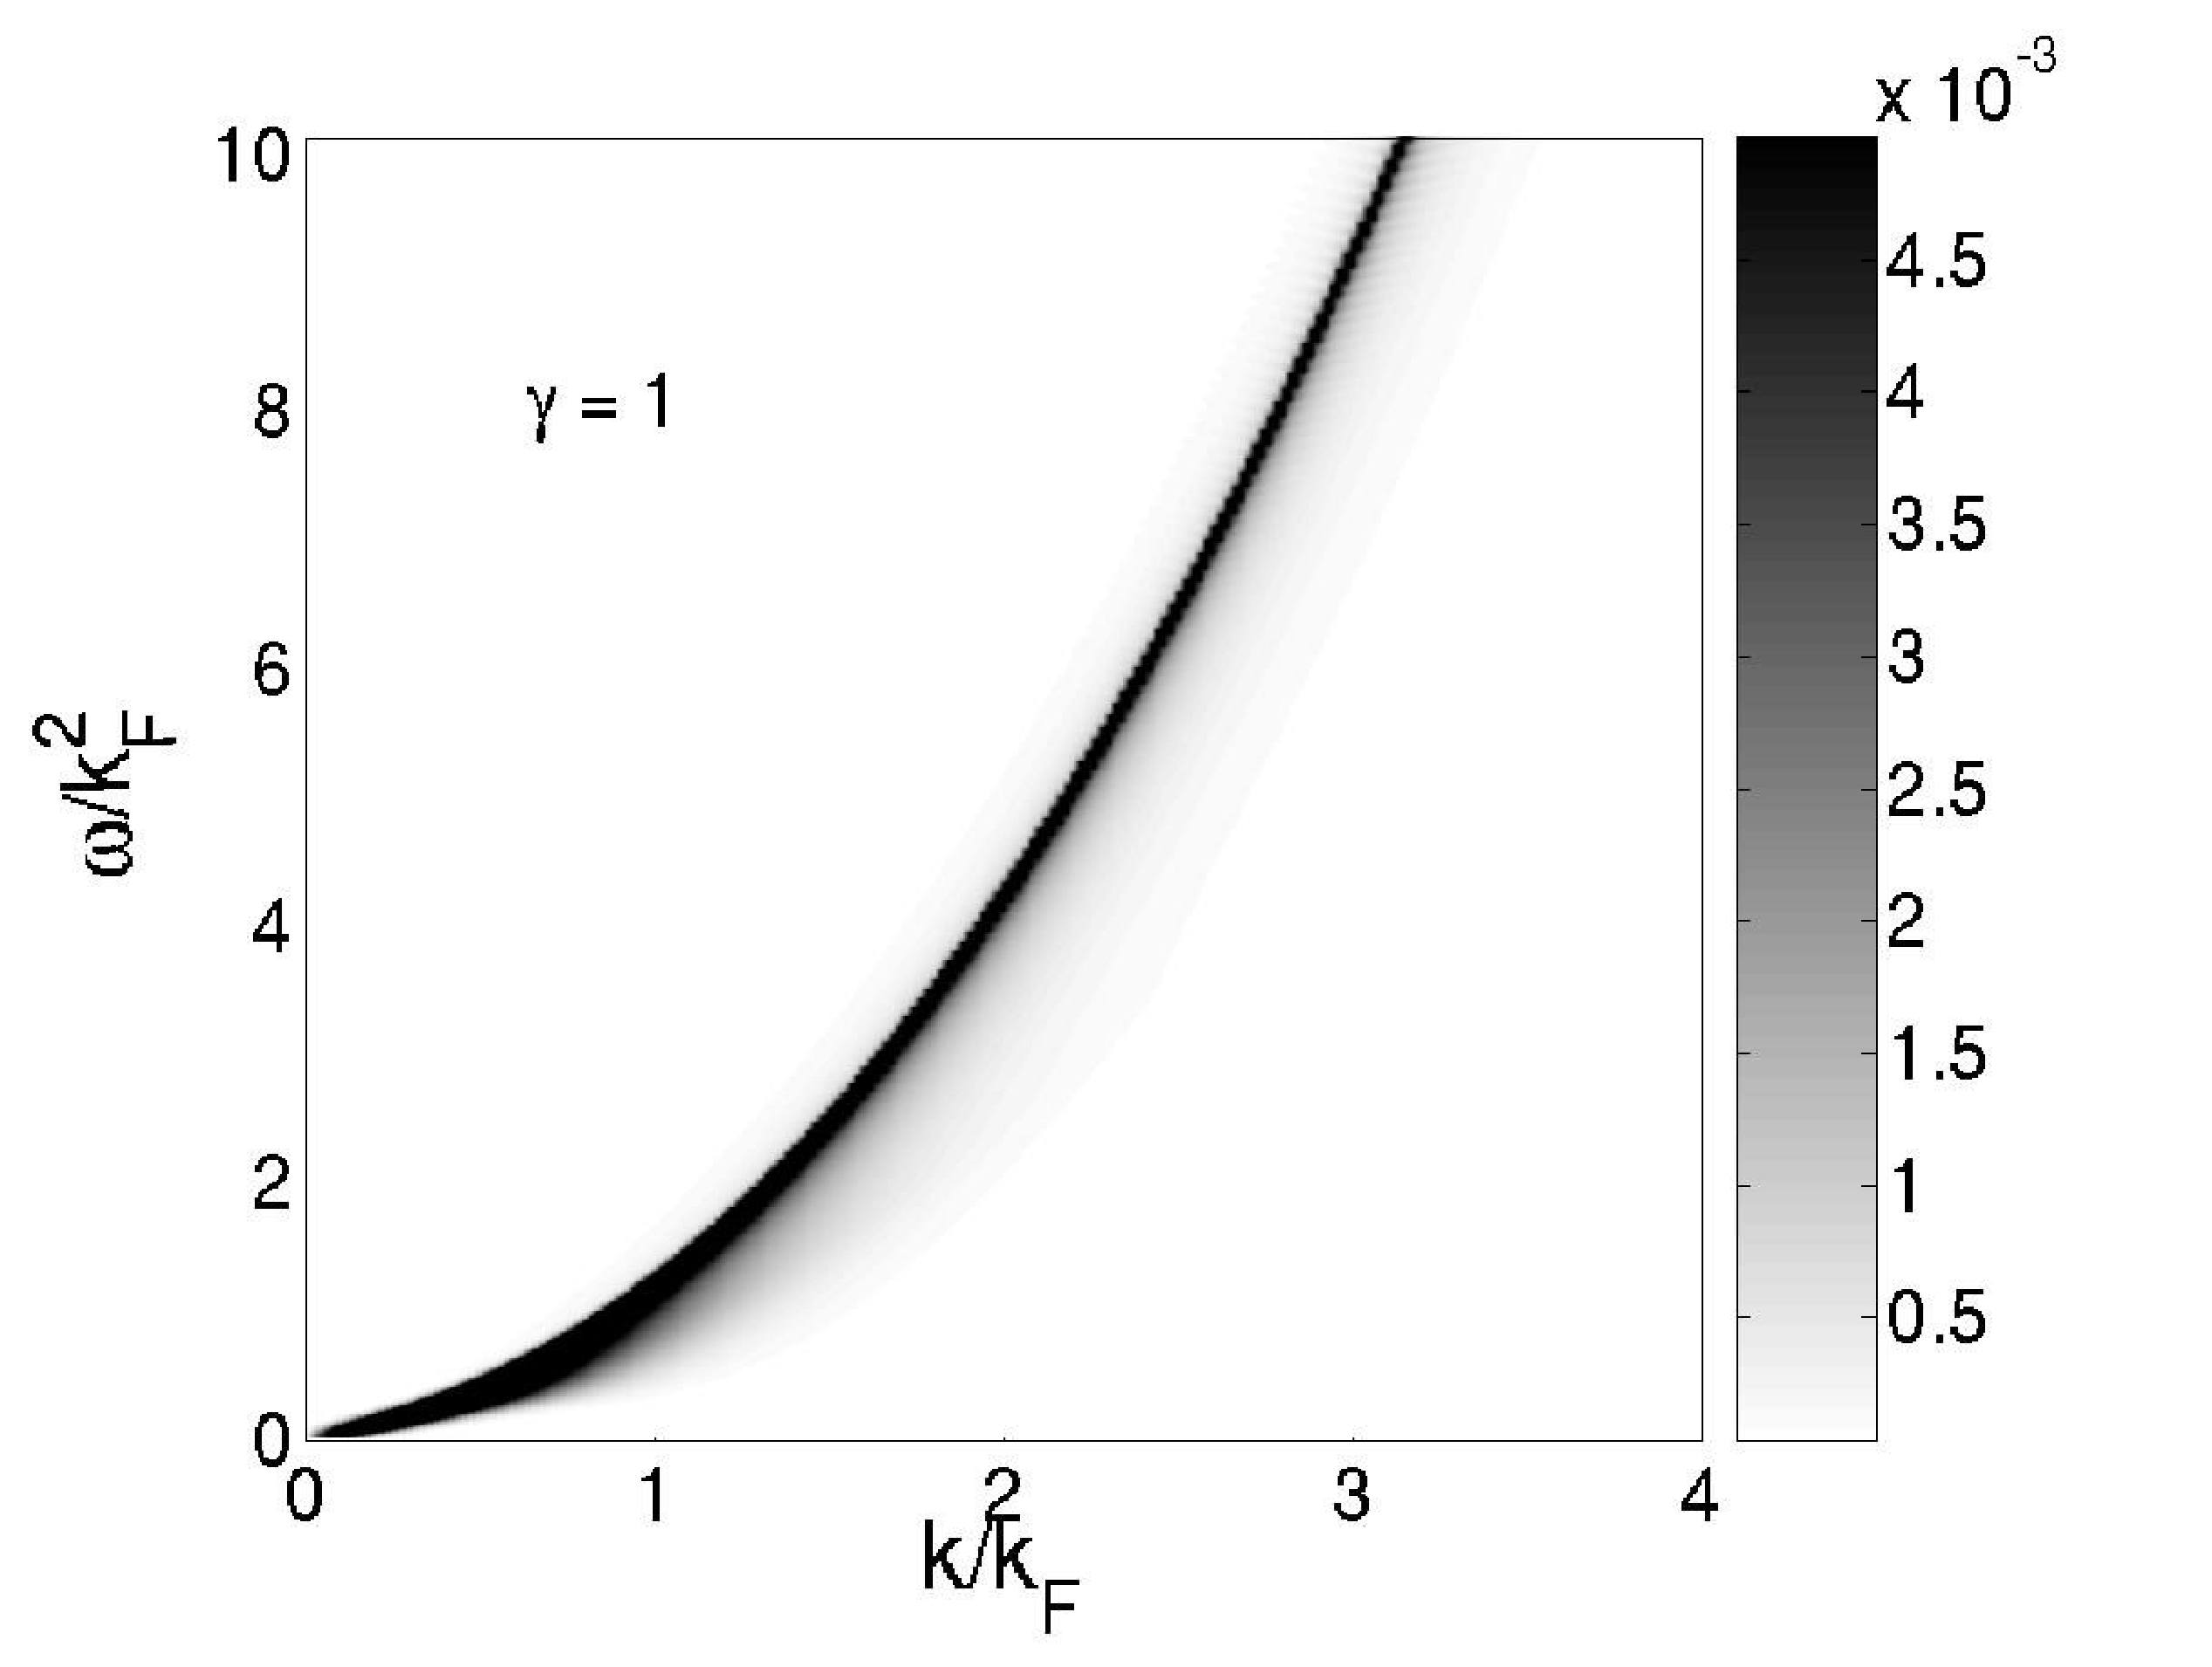
\includegraphics[width=4.3cm]{c_1_L_100_N_100.eps} \\
    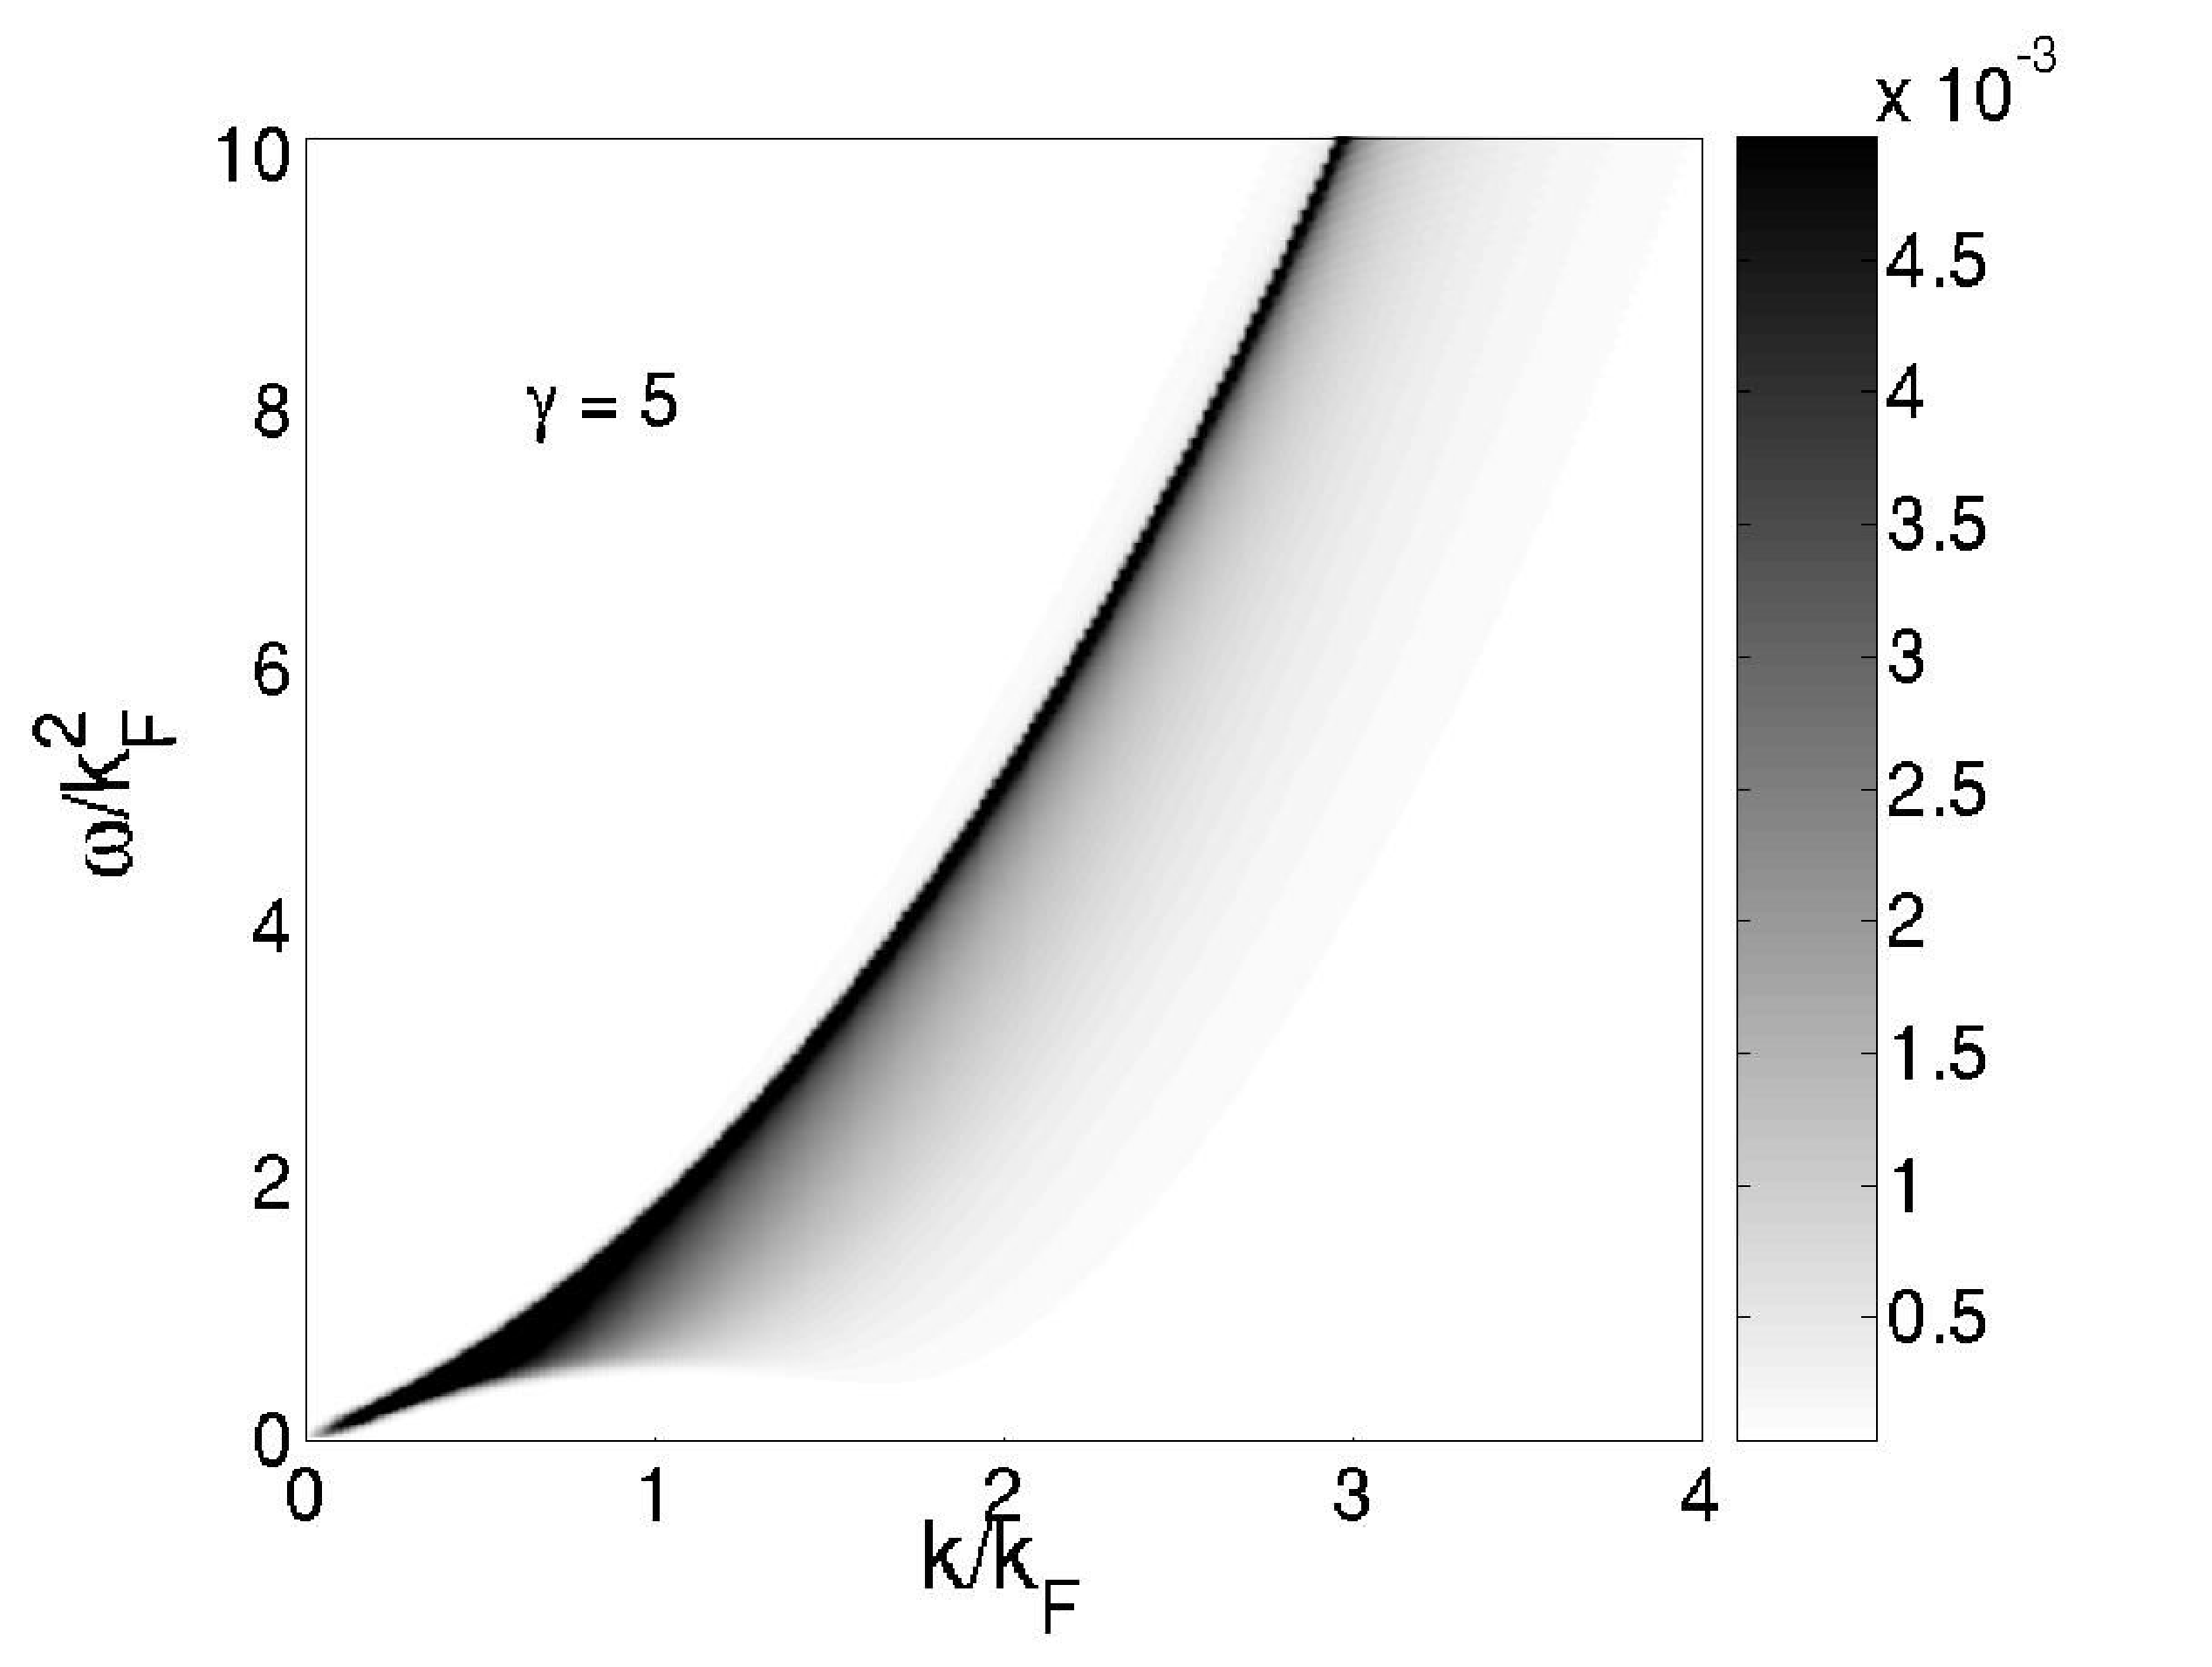
\includegraphics[width=4.3cm]{c_5_L_100_N_100.eps}
    &
      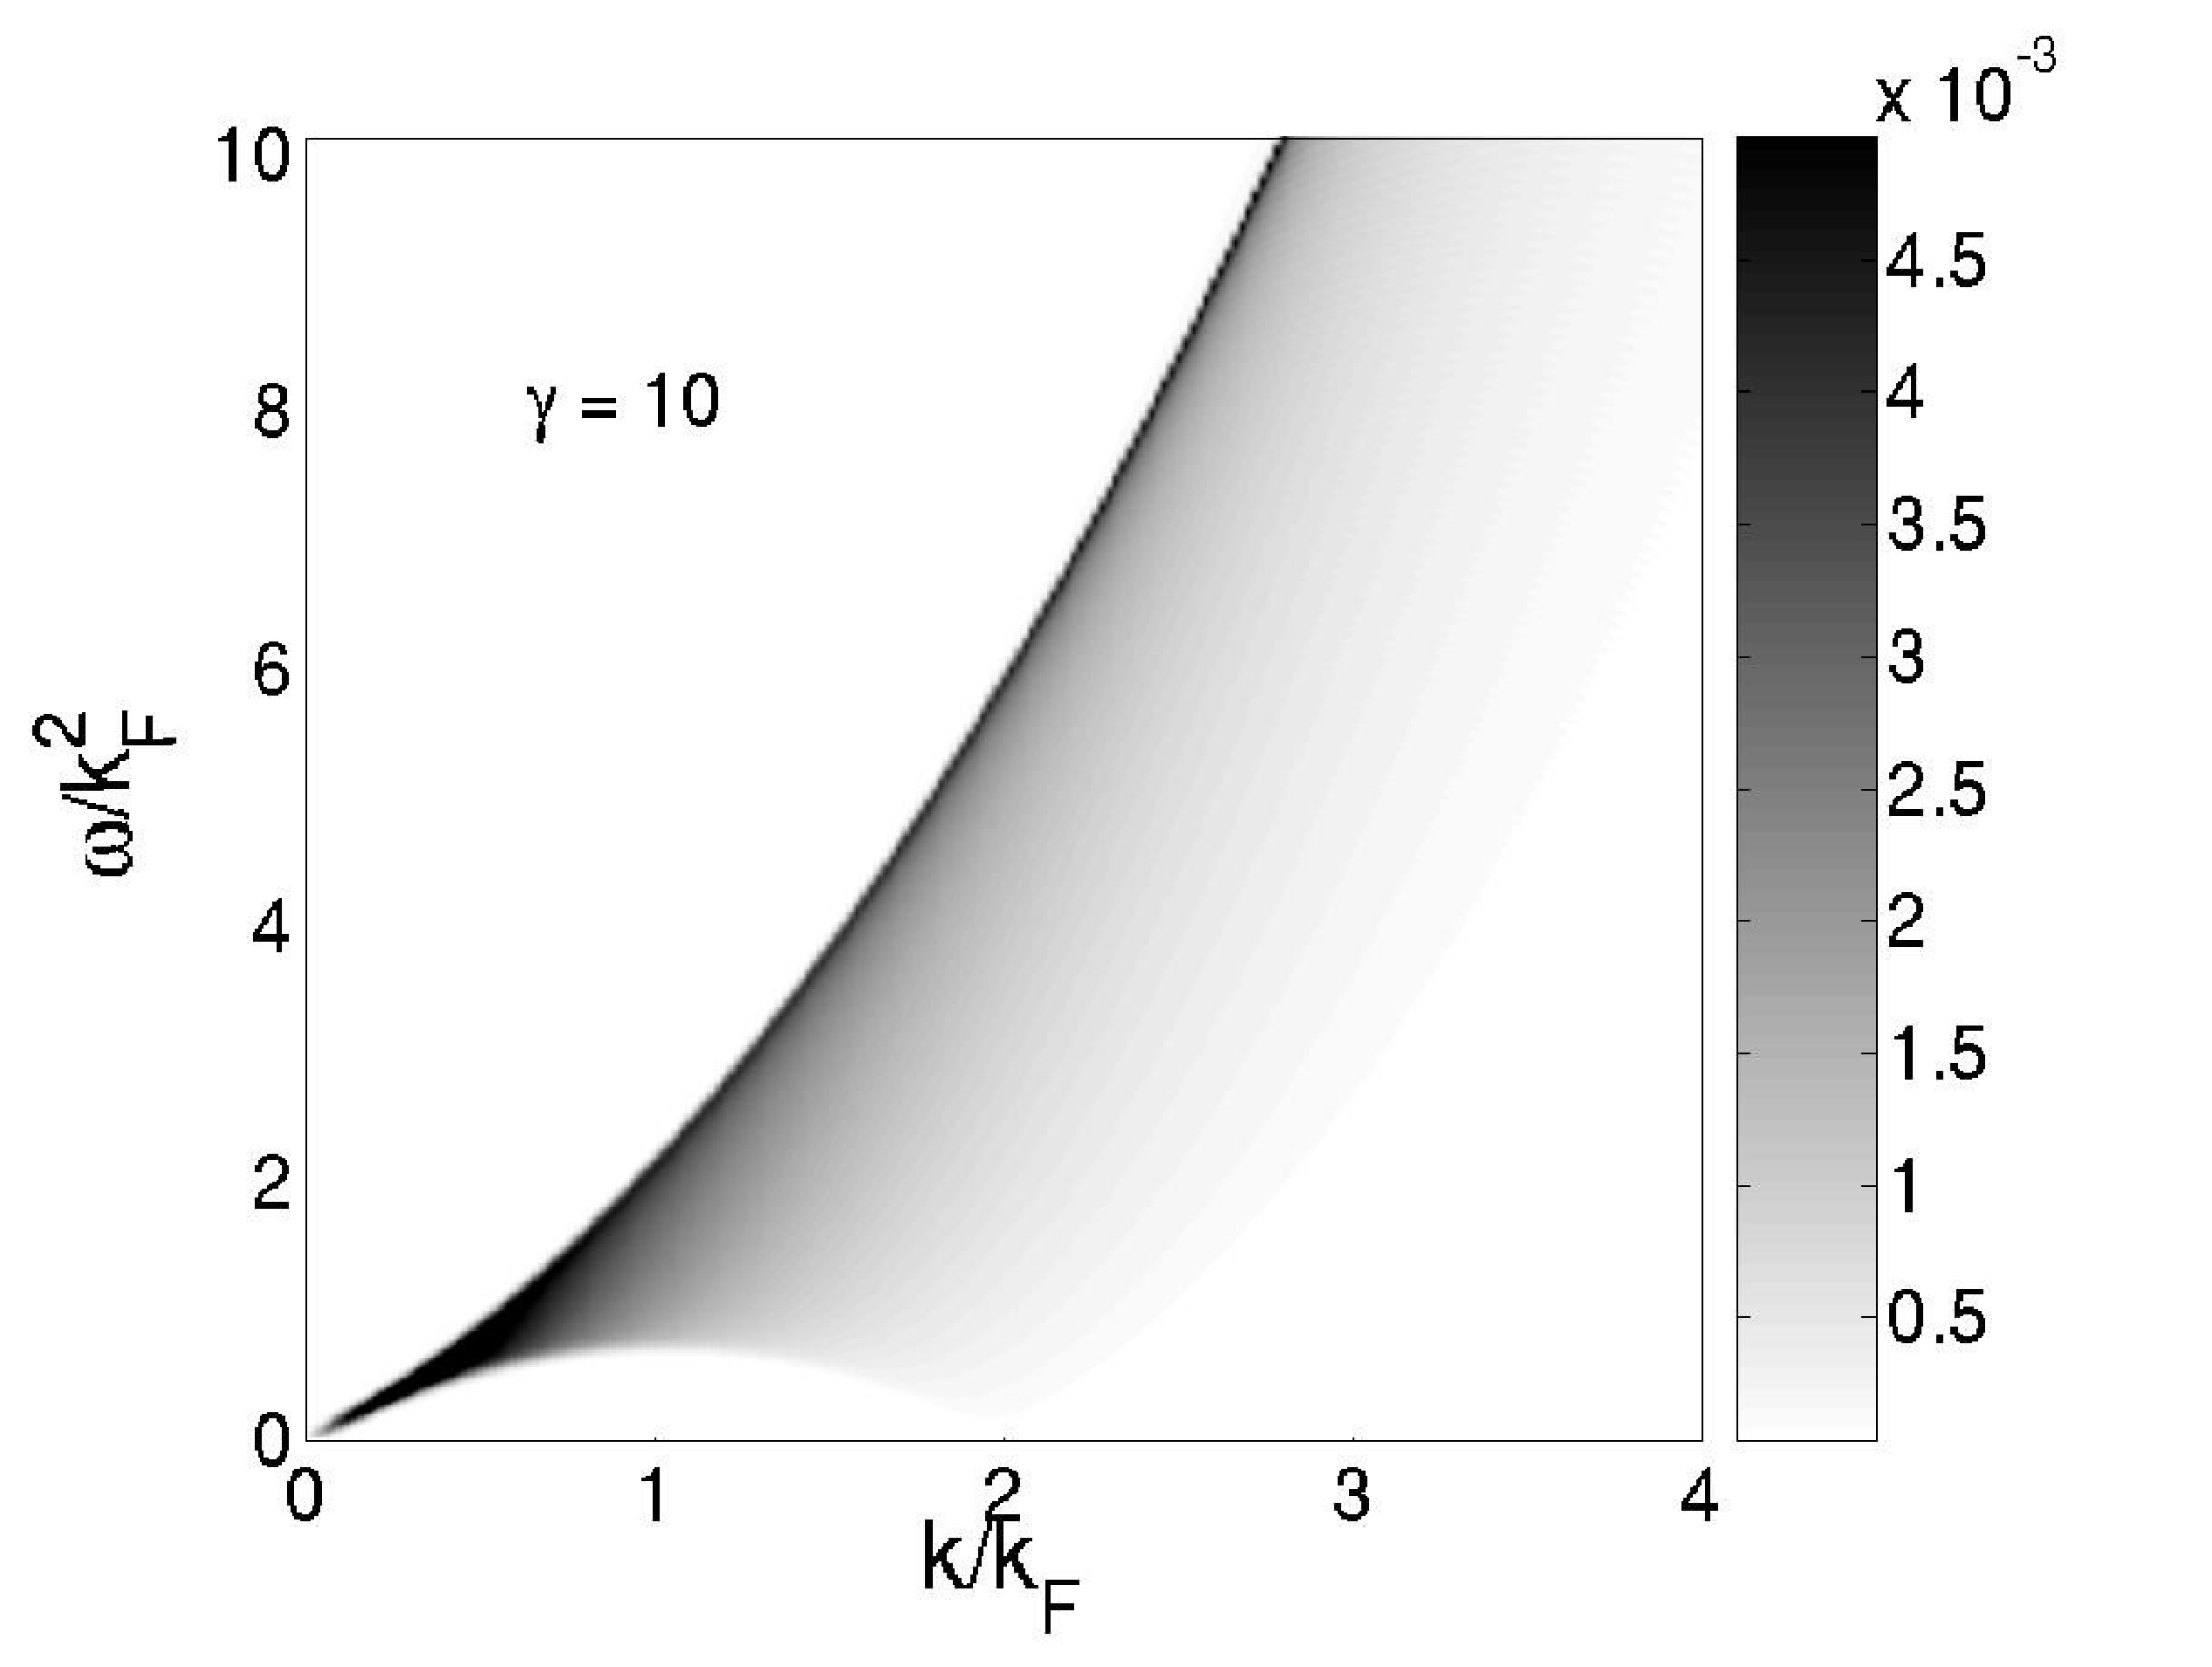
\includegraphics[width=4.3cm]{c_10_L_100_N_100.eps} \\
    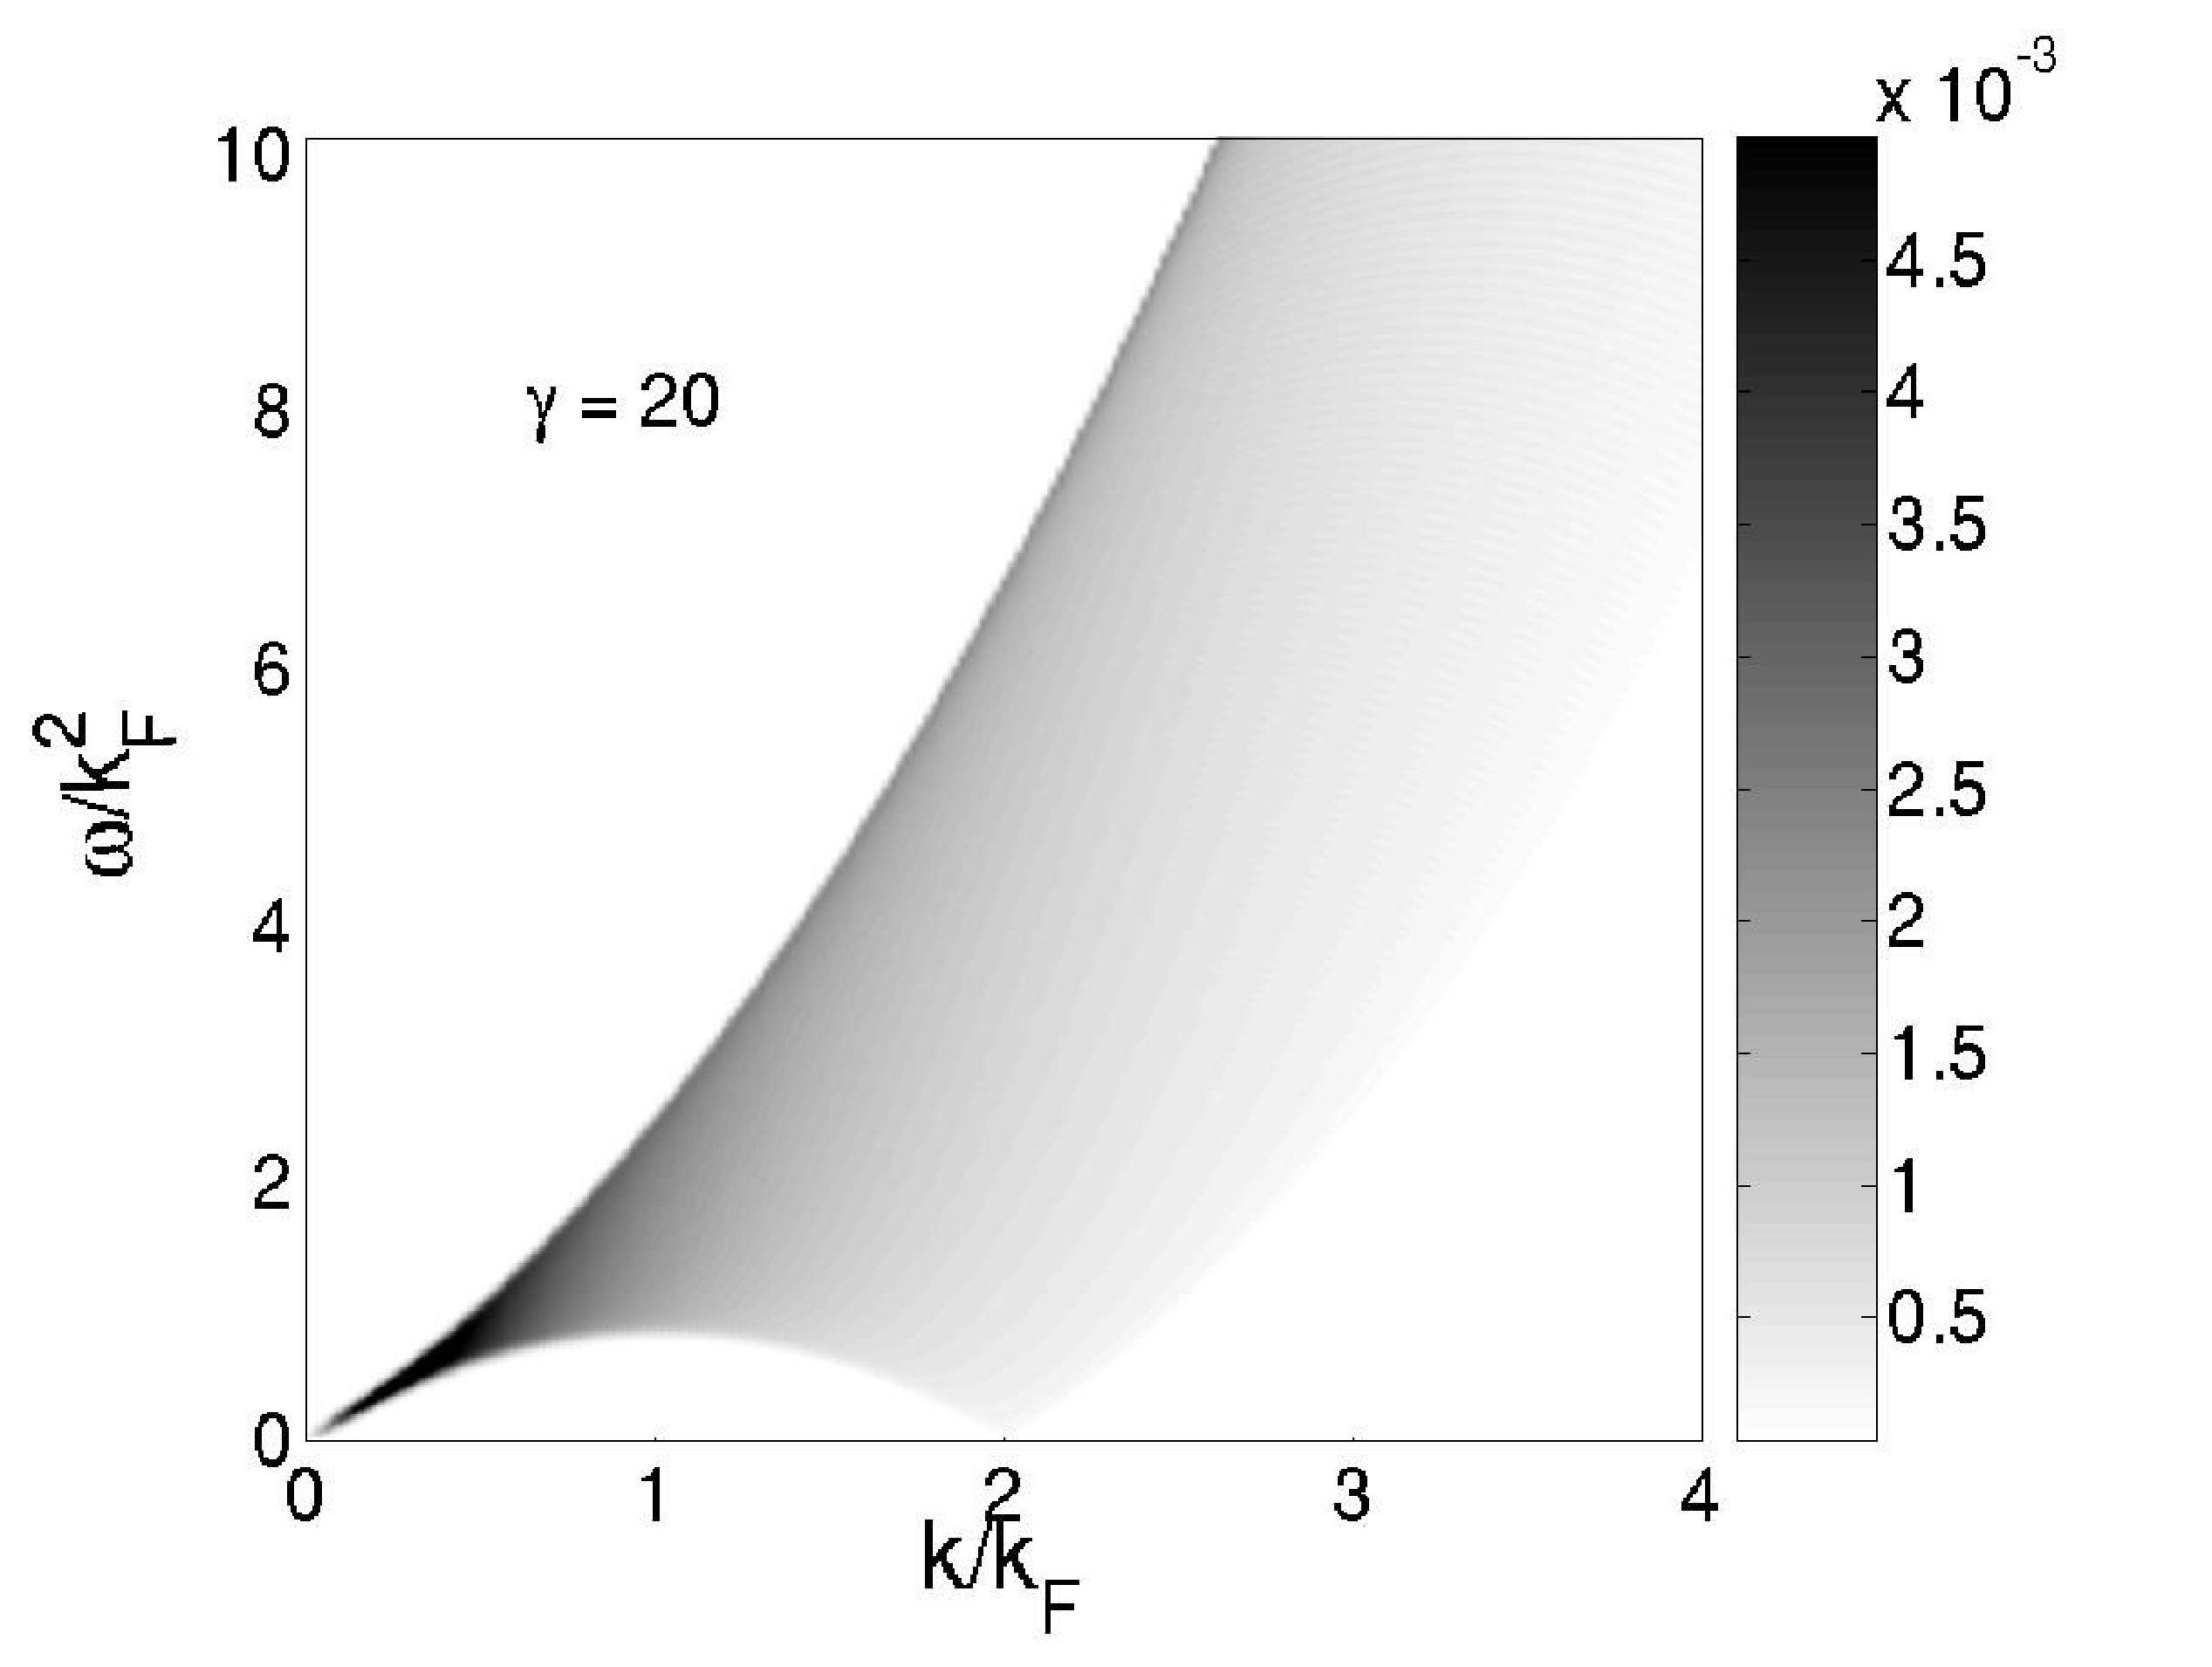
\includegraphics[width=4.3cm]{c_20_L_100_N_100.eps}
    &
      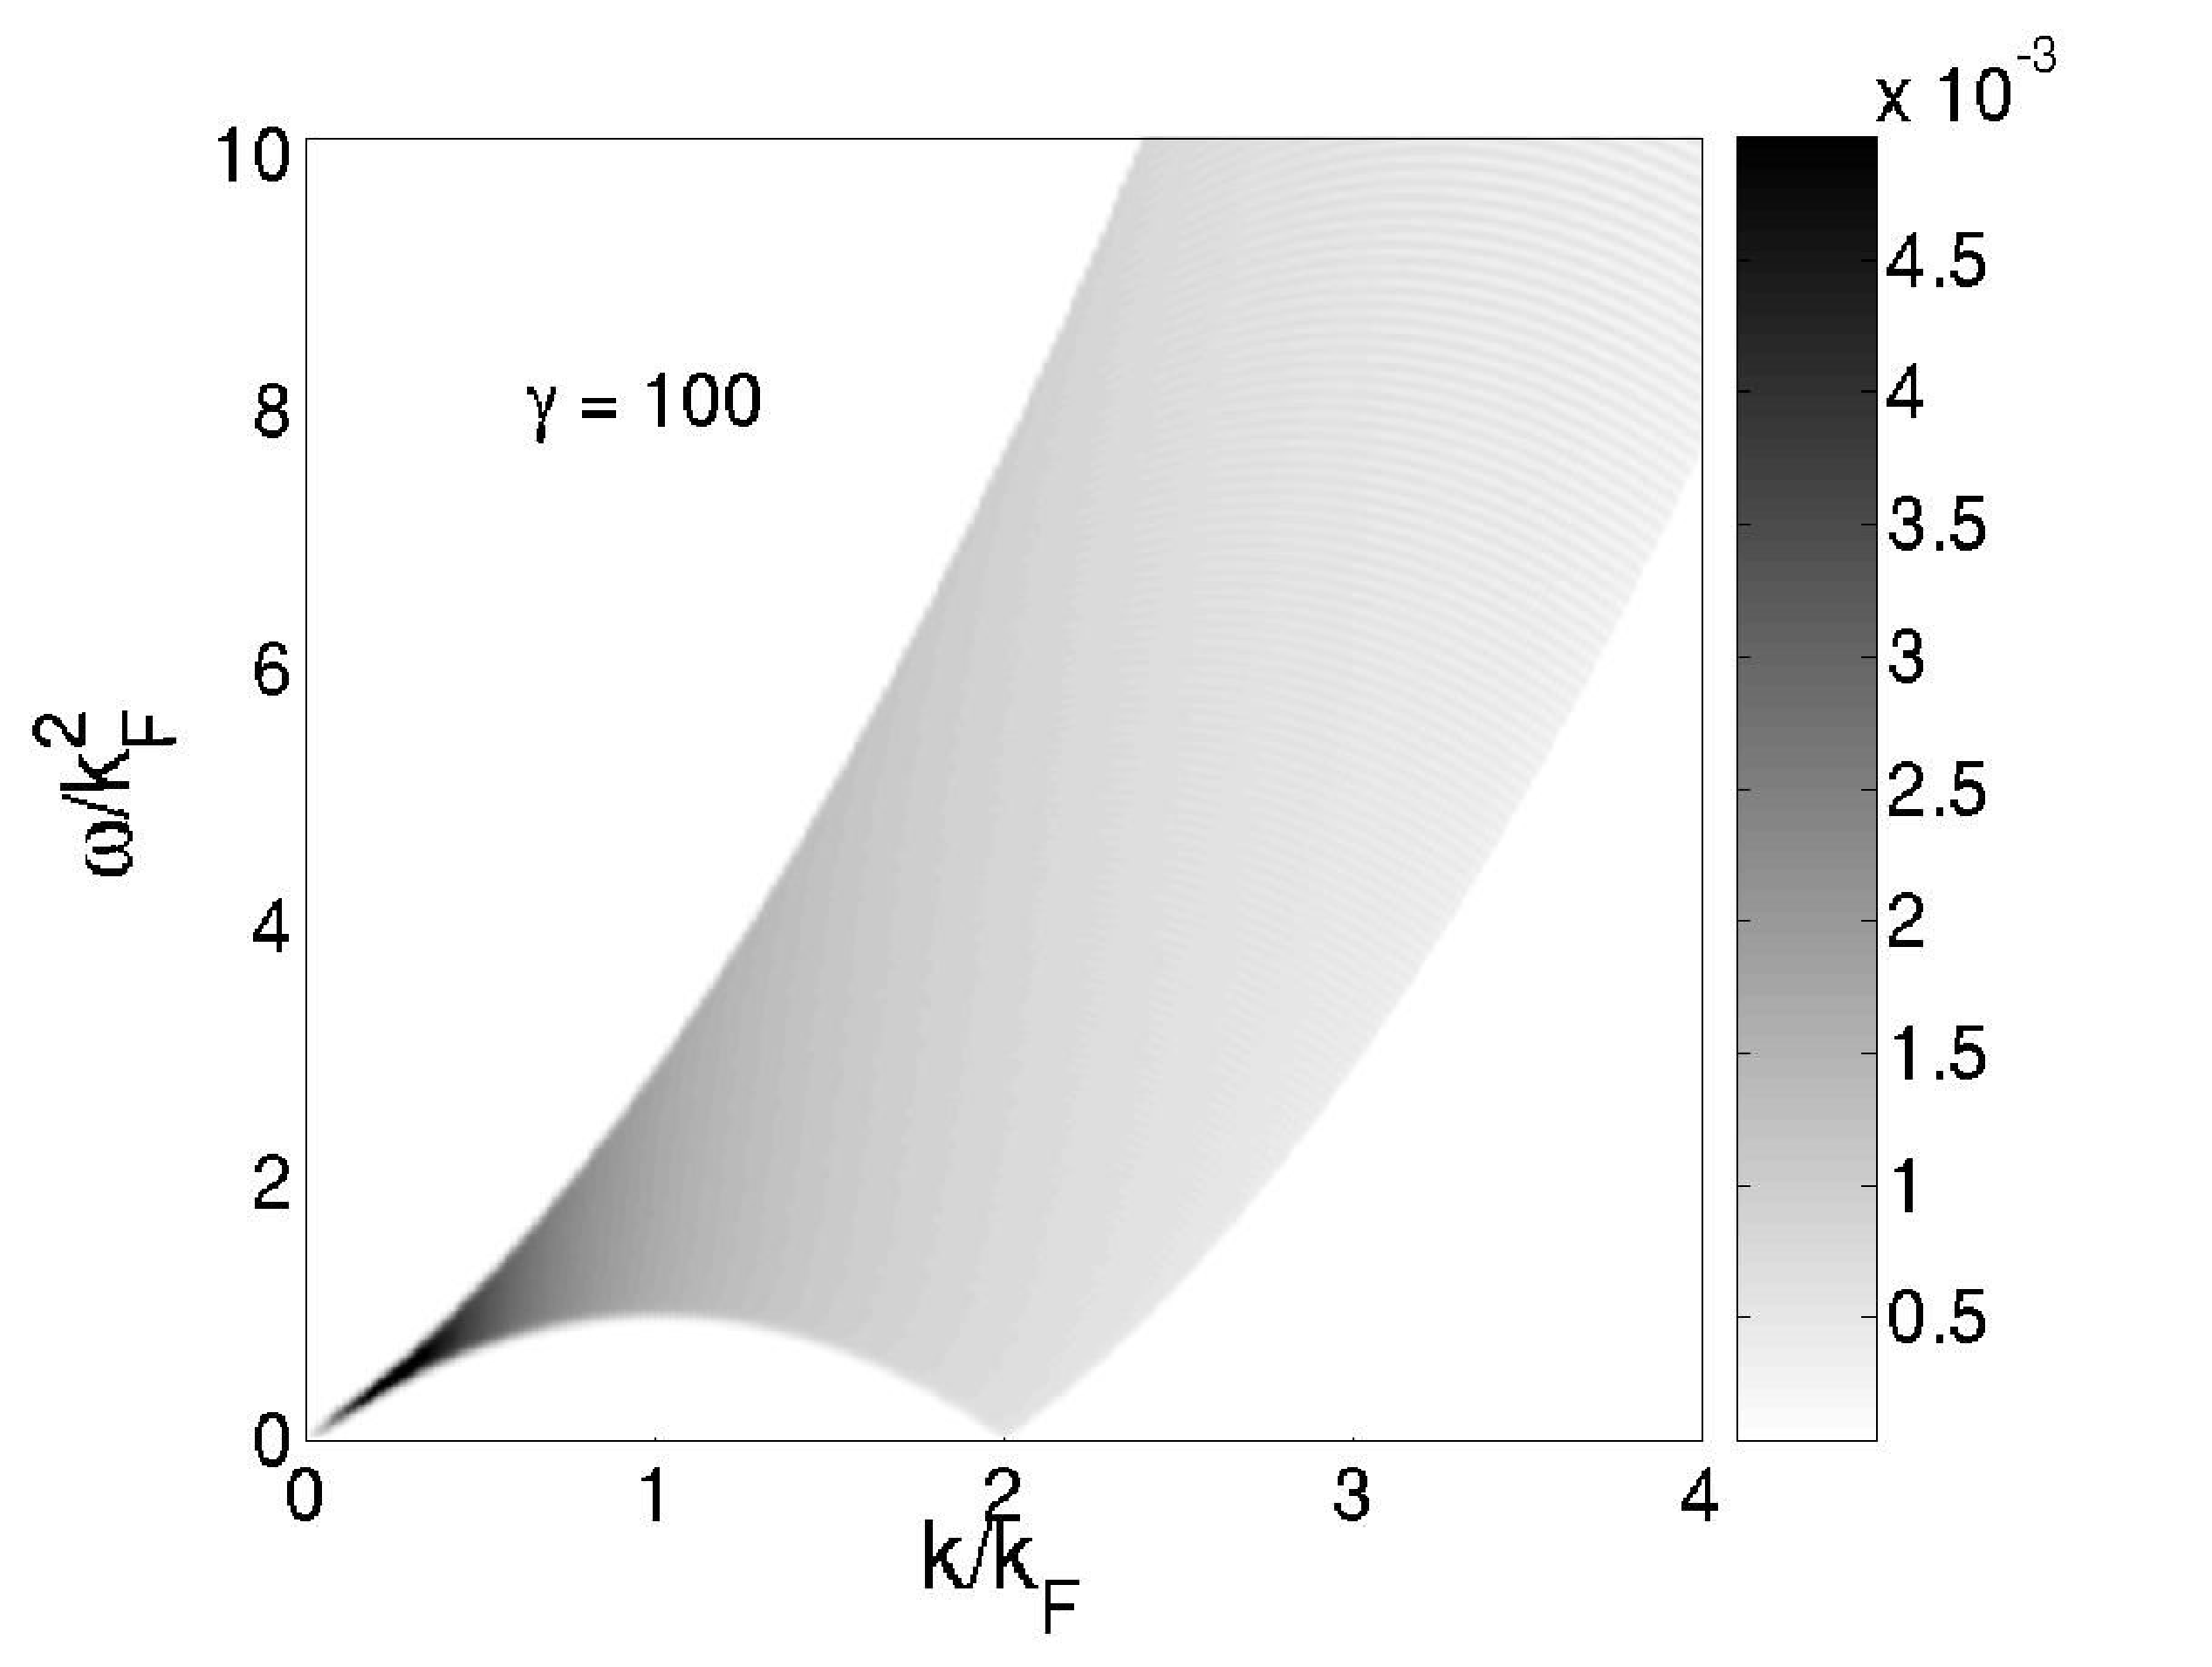
\includegraphics[width=4.3cm]{c_100_L_100_N_100.eps}
  \end{tabular}
  \caption{Plots of the dynamical structure factor of the Lieb-Liniger model for different values of the interactions parameter \(\gamma\).
    In this case we have $L = 100$ and $N = 100$.
    Figure taken from~\cite{Caux2007a}}
\label{fig:lieb_density_dsf}
\end{figure}


\begin{table}[tb!]
\centering
\resizebox{\textwidth}{!}{
\begin{tabular}{c|c|c|c|c}
  & N = 50 & N = 100 & N = 200 & N = 400 \\
\hline
90\% & 235 (\num{4.9e-12}) & 944 (\num{6.8e-26}) & 8772 (\num{5.3e-54}) & 117373 (\num{3.5e-111})\\
95\% & 385 (\num{8.2e-12}) & 2492 (\num{1.8e-25}) & 27096 (\num{1.6e-53}) & 573466 (\num{1.7e-110}) \\
99\% & 1515 (\num{3.2e-11}) & 18490 (\num{1.3e-24}) & 469120 (\num{2.8e-52}) & \\
99.9\% & 7478 (\num{1.6e-10}) & 141560 (\num{1.0e-23}) & & \\
99.99\% & 26724 (\num{5.7e-10}) & 932706 (\num{6.8e-23}) & & \\
% 90\% & 235 (4.9e-12; 40) & 944 (6.8e-26; 135) & 8772 (5.3e-54; 731) & 117373 (3.5e-111, 5175)\\
% 95\% & 385 (8.2e-12; 82) & 2492 (1.8e-25; 386) & 27096 (1.6e-53; 4319) & 573466 (1.7e-110; 34261) \\
% 99\% & 1515 (3.2e-11; 386) & 18490 (1.3e-24; 2500) & 469120 (2.8e-52; 16359) & \\
% 99.9\% & 7478 (1.6e-10; 1342) & 141560 (1.0e-23; 15366) & & \\
% 99.99\% & 26724 (5.7e-10; 2182) & 932706 (6.8e-23; 84047) & & \\
\end{tabular}
}
\caption{Number of states required for a given sum rule saturation in the XXZ model with \(\Delta=0.6\) and \(S_{\mathrm{tot}}^z=0.1\).
In parentheses are the fraction Hilbert space fraction this represents.
% with the second number in parentheses the number of contributions needed if the algorithm was perfectly able to only sum monotonically decreasing form factors.
Table reproduced from~\cite{Caux2009}.
}
\label{table:saturation}
\end{table}

\begin{savequote}[50mm]
Real stupidity beats artificial intelligence every time.
\qauthor{Terry Pratchett, Hogfather}
\end{savequote}


\chapter{Machine learning techniques}\label{chap:machine_learning}

% \epigraph{\textit{Real stupidity beats artificial intelligence every time.}}{Terry Pratchett, Hogfather}
\noindent
\section{Machine learning in physics}

In the past decade machine learning has emerged as an important tool in many areas.
The increase in computing power for both CPUs and GPUs (useful for parallel linear algebra often used in machine learning) has led to a boom in research on both the commercial and academic side.
Some of the more high profile examples of this are self-driving cars (being developed by many technology and car companies)~\cite{levinson11_towar} and the development of AlphaGo, which beat the world champion in the Japanese board game of Go by learning from both human professional games and playing against itself~\cite{Silver2017a,Silver2017,silver16_master_game_go_with_deep}.
In the life sciences machine learning uses include detecting risk factors for cardiovascular diseases from pictures of the retina~\cite{poplin17_predic_cardiov_risk_factor_from} and recognizing genome variants in sequencing (with better performance than handcrafted sequencers)~\cite{Poplin2016}.
Image manipulation is also benefitting from machine learning, with the ability to change the weather in pictures or transfer the species of animal in one picture to that in another~\cite{Liu2017}.

In physics applications have also been found in a variety of fields.
CERN is exploring ways of tagging particles in LHC collisions using deep learning~\cite{paganini17_machin_learn_algor_jet_taggin}.
In astronomy machine learning is used to classify objects in images and determine redshifts, which have to be automated due to the often large data sets resulting from even a single night of observations~\cite{ball10_data_minin_and_machin_learn_in_astron}.

Condensed matter physics is now also benefitting from this field.
Recently, Carleo and Troyer~\cite{Carleo2017} proposed a way to find the ground state wave function of various spin systems by approximately encoding the state of a system in a neural network. This allows for accurate approximations of the ground state energy while avoiding the exponential number of parameters encountered when representing the Hilbert space.
This technique has been extended to different systems such as the Hubbard model~\cite{Saito2017}.
Phase transitions and order parameters have also been successfully extracted from both static and periodically driven systems, using only measurable quantities such as the magnetization of individual spins~\cite{Nieuwenburg2017}.

Reinforcement learning has been used to design setups for optical experiments in which complex entangled states are needed.
Since the setups are often difficult to design, reinforcement learning is used, where the computer receives a reward if an `interesting' state is created~\cite{Dunjko2017}.

There are also interesting links between deep learning and physics on a more fundamental level.
For example, an exact mapping was established between the variational renormalization group en deep learning, implying that deep learning works by extracting relevant data features in a similar way to the renormalization group~\cite{Mehta2014}. 

In the rest of this chapter we will review some aspects of machine learning useful in the ABACUS algorithm.\footnote{Note that we always talk here about applying machine learning to quantum mechanics, not about machine learning on quantum computers (see~\cite{Dunjko2017}).}


\section{Machine learning: the basics}
In many cases we would like to find patterns in data.
The 

\subsection{Neural networks}
Stochastic gradient descent
training, validation, testing
Feedforward
\cite{Bishop2006}

\section{Reinforcement learning}

The machine learning techniques we have described until now all rely on large data sets to function, being supervised algorithms.
They use expert data to train and this (hopefully) allows for generalization to new data.
In many cases however the acquisition of expert data is difficult or impossible.
In these cases reinforcement learning comes into play.
Here, there is no a priori knowledge of the targets, only a reward function that, given a state and an action returns a reward.

\subsection{Q-learning}

model free, off-policy

sgd used~\cite{mnih13_playin_atari_with_deep_reinf_learn}




\cite{Sutton}

\begin{savequote}[50mm]
If you torture the data long enough, it will confess anything.
\qauthor{Ronald Coase}
\end{savequote}


\chapter{Methods and results}\label{chap:results}

% \epigraph{\textit{}}{}
\noindent

Now that we have introduced the theoretical tools necessary, we can combine them in a way applicable to integrable models.
We start with simple regression to find rapidities and then turn to exploring the state space of the Lieb-Liniger model.
All neural networks and code were written in Python, with the neural networks using the Keras framework~\cite{chollet2015keras} with Tensorflow backend~\cite{tensorflow2015-whitepaper}.

\section{Regressing rapidities}

As discussed (\cref{chap:bethe_ansatz}), rapidities play a central role in Bethe ansatz integrable models.
They form the basis for calculations of form factors and quantities such as the energy of a system.

We have also seen how rapidities may be found numerically in~\cref{sec:numer-solv-bethe}, using the (multidimensional) Newton method.
This method converges quadratically, but requires an initial guess for the rapidities.
It is here that we may find an improvement by way of machine learning.

In the naive case, where we simply start from scratch in calculating the rapidities, we base the initial values for the Newton method on a simplified first order version of the Bethe equations (\cref{eq:bethe_equations}):
\begin{align}
  \label{eq:12}
  \lambda_j = \frac{2\pi}{L} I_j.
\end{align}

We expect the number of iterations required for convergence of the Newton method to be reduced if the initial values are closer to their true values.
Therefore, we use a neural network to act as a function approximator, feeding in an array of \(N\) Bethe numbers and outputting an array of \(N\) rapidities.

The methodology is as follows: we generate a data set of 20000 sets of Bethe numbers and calculate their corresponding rapidities of length \(N\), for various values of \(N\).
The Bethe numbers are randomly drawn from a normal distribution centered on 0, with a variance of \(N\) (this corresponds to biasing the generated states to be close to the ground state).
There is no additional UV cutoff employed.

The generated data is used for training a neural network consisting of an input layer of size \(N\), two hidden layers of size \(N^2\) and an output layer of size \(N\).
Apart from the output layer all layers use a hyperbolic tangent activation function.
This architecture was arrived at through trial and error.
More complex networks showed did not show improvements on rapidity estimation and took longer to train and to evaluate.

\subsection{Results}
We compare 4 different ways of determining initial values: using \cref{eq:12} (denoted as ``Naive Bethe''), using the neural network described above (denoted ``ML''), using a vector of random numbers drawn from a normal distribution with mean 0 and variance \(N\) (``Random'') and a vector of random numbers drawn from a normal distribution with mean 0 and variance \(N\) where entries are sorted (``Random sorted'').

We also compare all these methods with both damping (\cref{eq:dampednewton}) enabled and disabled. We use systems with \(c=1\) and \(L=N=5,10\) and 20.
Of the 20000 data points, 19000 are used for training and 1000 for validation over 100 training epochs.

We observe that the neural network learns the structure of the rapidities reasonably well, notably learning part of \cref{th:equalisequal}: if \(I_j >I_k\), then \(\lambda_j > \lambda_k\) (see \cref{fig:rapidities}).

\begin{figure}[tb]
  \centering
  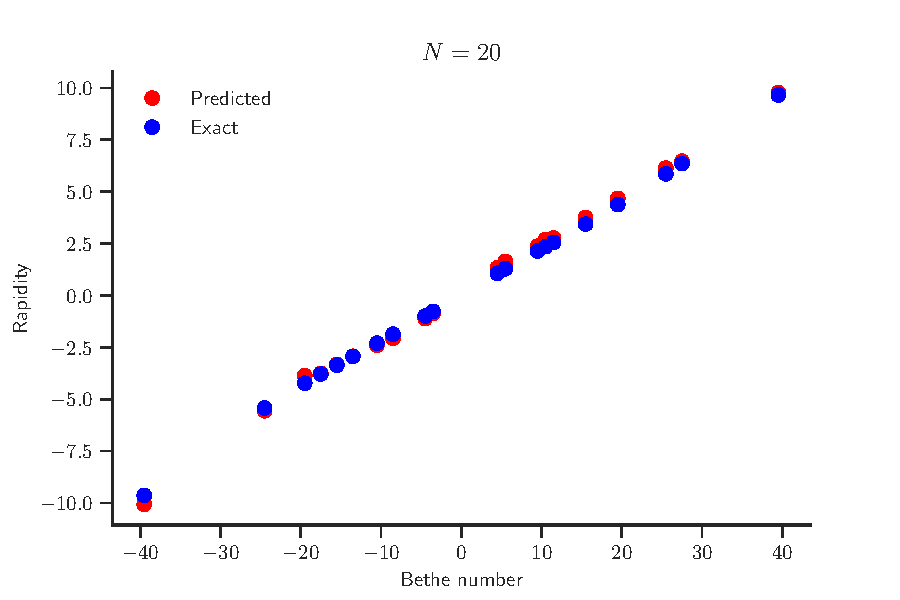
\includegraphics[width=0.70\textwidth]{rapidities_20.pdf}
  \caption{Predicted and exact rapidities for the Lieb-Liniger model with \(c=1\), \(L=N=20\).}
  \label{fig:rapidities}
\end{figure}

The real question however is whether the initial guesses of the neural network are better than those of the Naive Bethe approach.
Comparing different initial guess methods in \cref{fig:iterations}, we see this being the case.
We compare the average number of iterations to convergence over 1000 sets of Bethe numbers for each method.
The difference between Naive Bethe and ML is most pronounced for \(N=5\), being on average \(0.95\) iterations.
This difference decreases to \(0.43-0.45\) iterations for \(N=10\) and to \(0.07-0.09\) iterations for \(N=20\).
This decrease is probably due to the inability of the neural network to capture the increasing number of cross interactions of the rapidities with increasing system size.
Compared to random initialization (either sorted or unsorted), both Naive Bethe and ML perform better.
We see that sorting random initial values improves convergence, probably because a sorted list of monotonically increasing initial values captures the basic structure of the rapidities.
Damping does not appear to have a large impact on convergence and we will from here on only consider undamped rapidity calculations.

Comparing time until convergence paints a different picture compared to that above.
Looking at \cref{fig:convtimes} we see that the ML method is consistently slower than Naive Bethe, although the difference decreases as \(N\) increases.
This is probably because during Newton iterations we use LU decompositions, which have an algorithmic complexity \(\mathcal{O}(N^3)\)~\cite{Press2007}.
For large \(N\) this step outweighs the increased complexity introduced by the neural network compared to a naive guess, because the number of calculations necessary for evaluation in the neural network is determined by the number of parameters and is therefore of order \(\mathcal{O}(N^2)\).
This also explains why the random initializations are generally slower. 
The increased number of iterations with their associated operations of \(\mathcal{O}(N^3)\) makes reaching convergence take longer.
Note that the durations in \cref{fig:convtimes} for machine learning do not capture the time required for data set generation and training, making the actual times required to get predictions for the rapidities longer than those reported.
Machine learning thus does not aid in determining rapidities more efficiently.

The raw values reported in \cref{fig:iterations} and \cref{fig:convtimes} may be found in \cref{cha:rawvalues}.

\begin{figure}[ph]
  \centering
  \subfloat{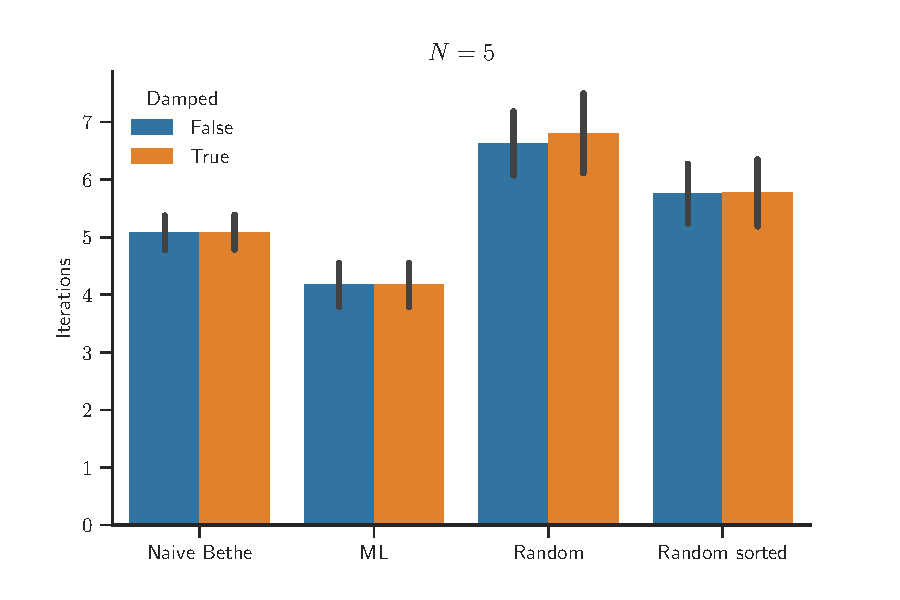
\includegraphics[width=0.70\textwidth]{iterations_5.pdf}}\\
  \subfloat{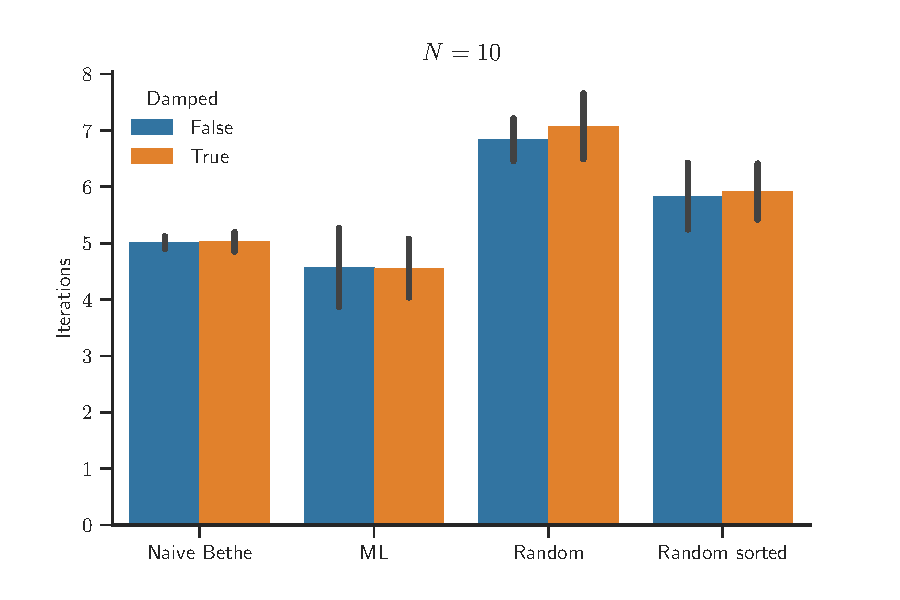
\includegraphics[width=0.70\textwidth]{iterations_10.pdf}}\\
  \subfloat{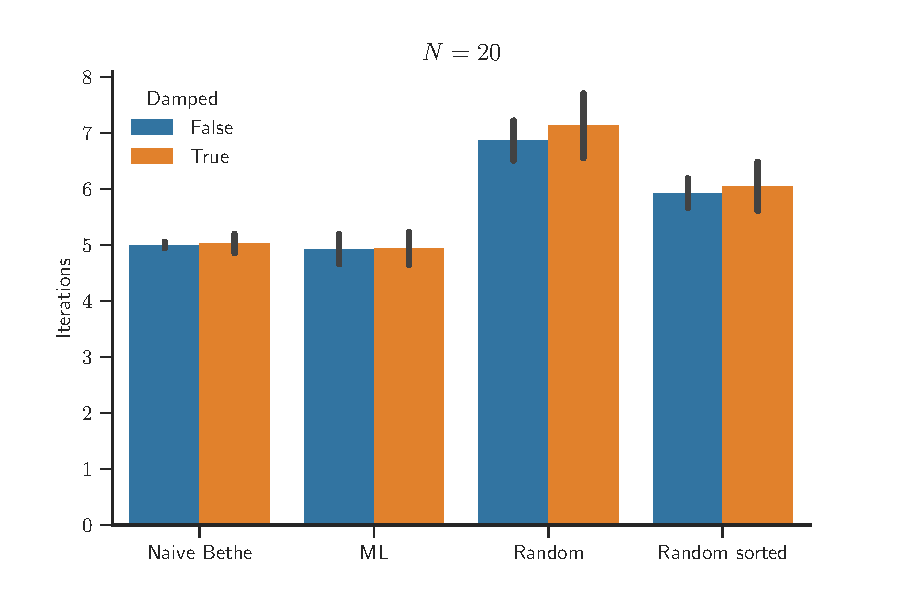
\includegraphics[width=0.70\textwidth]{iterations_20.pdf}}
  \caption{Number of Newton iterations until convergence is reached for \(N=5,10,20\), averaged over 1000 sets of Bethe numbers. The black bars denote standard errors.}
  \label{fig:iterations}
\end{figure}

\begin{figure}[ph]
  \centering
  \subfloat{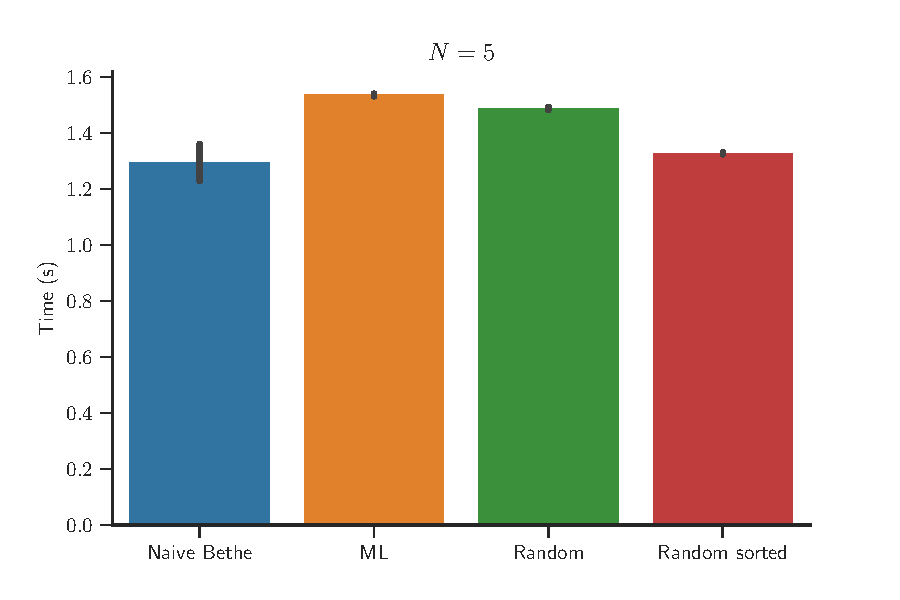
\includegraphics[width=0.70\textwidth]{time_5.pdf}}\\
  \subfloat{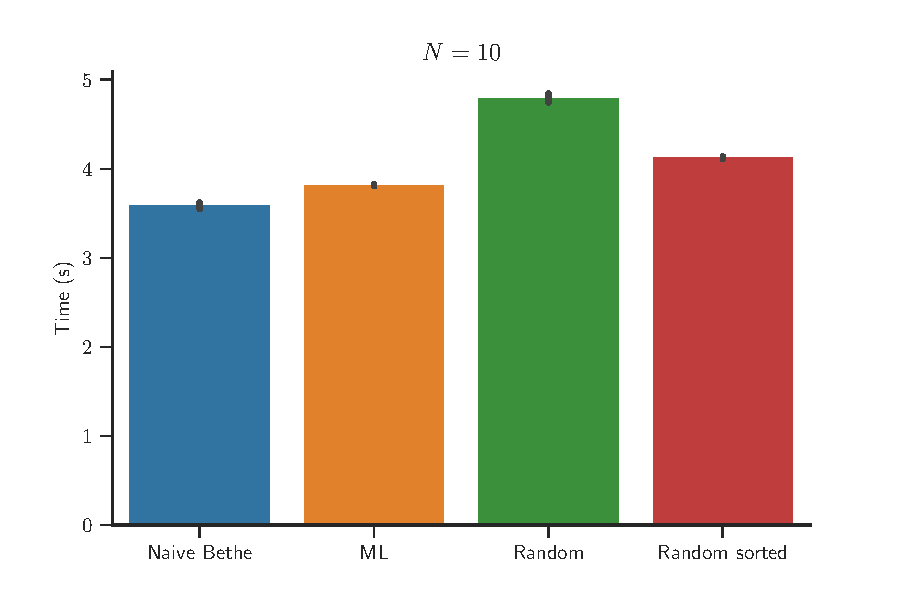
\includegraphics[width=0.70\textwidth]{time_10.pdf}}\\
  \subfloat{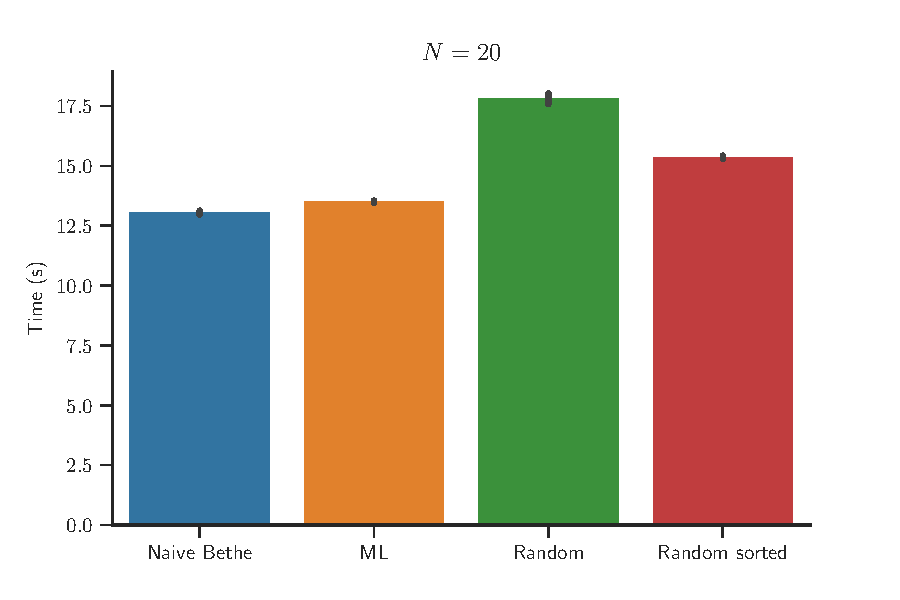
\includegraphics[width=0.70\textwidth]{time_20.pdf}}
  \caption{Time in seconds until convergence is reached for \(N=5,10,20\). We average over 10 runs of 1000 sets of Bethe numbers. The black bars denote standard errors.}
  \label{fig:convtimes}
\end{figure}

\section{Walking through state space}

We now turn to exploring the state space of Bethe integrable models using machine learning.
What we are in general interested in is that, given a starting point in state space (usually the ground state), we want to explore the state space in the most efficient way possible.

Recalling the Lehman representation of the dynamic structure function (DSF, \cref{eq:lehman})
\begin{equation}
  \mathcal{S}(k,\omega) = \frac{2\pi}{N}\sum_{\mu}\abs{\mel{\lambda^0}{\mathcal{O}_k}{\mu}}^2 \delta(\omega-E_{\mu}+E_0), 
\end{equation}
we note that if we want to evaluate the above expression, we in principle have to sum over the entire Hilbert space of the model in question (potentially a space of  infinite size) to capture all behaviour of the DSF.
Due to the impracticality of this we instead consider states that contribute a lot to the above sum.
In general these are states with a large matrix element.
More precisely they are states with large contributions to the f-sum rule (see \cref{eq:fsumrule}):
\begin{align}
  \frac{1}{N}\sum_{\mu}(E_{\mu}-E_0)\abs{\mel{\lambda^0}{\rho}{\mu}}^2  = \frac{N}{L} k^2,
\end{align}
where we specified to the case of the density operator \(\rho = \Psi^{\dag}\Psi\) for the Lieb-Liniger model.
This allows us to determine which fraction of states have been summed in a given slice of momentum \(k\).

At present the scanning of the Hilbert space is implemented in ABACUS in the form of a large function of approximately 600 lines, using heuristics and the method outlined in \cref{chap:abacus} to capture important states as much as possible.
Looking at \cref{fig:orderedmagnitudes}, we see that the summation is not yet optimal, in that some important states are not captured early in the summation.
This results in lower than possible saturation of the f-sum rule for a given running time of ABACUS.

We therefore turn to machine learning to scan through the Hilbert space in a hopefully more efficient way.
This also moves complexity from the handcrafted function into a neural network.
While the neural network in more opaque in how it arrives at solutions, it may nevertheless present a more systemic way of arriving at an algorithm.

We use reinforcement learning as a way to iteratively come to an optimal state summation, inspired by the recent success of Google Deepmind in playing Go~\cite{silver16_master_game_go_with_deep,Silver2017a}, chess and shogi~\cite{Silver2017} and 1980s computer games~\cite{mnih13_playin_atari_with_deep_reinf_learn,mnih15_human_level_contr_throug_deep_reinf_learn}.
The methods of these papers are especially notable because they do not require handcrafting the inputs to the neural networks, but learn higher level representations from scratch.
Specifically we will use Q-learning as in the last two references.
We refer to \cref{chap:machine_learning} for an general explanation of Q-learning and focus here only on the specifics relevant to Hilbert space scanning of the Lieb-Liniger model.
Note that the learning we employ is tabula rasa, meaning that there is no pretraining on a known data set and all learning occurs from scratch.

\subsection{State and move representation}

When using neural networks we need a concrete representation of the state.
A vector of Bethe numbers has a resolution that is too low as it hides some of the degrees of freedom of the system, notably not covering the holes that appear between particles.
We therefore use a binary encoding for Lieb-Liniger model states, mapping the Bethe numbers to a vector where 1s represent particles and 0s represent empty locations in Bethe number space.
Because the vector has to have a finite size this representation does force us to implement a UV-cutoff above which there are no Bethe numbers and which can not be occupied.
We call this cutoff \(I_{\max}\).
States in binary representation are then vectors of length $N_{\textrm{world}} = 2 I_{\max} + 1$.
For example, the ground state of the $N=3$ state with $I_{\max} = 5$ is\footnote{Due to rounding errors when considering the half-integer Bethe numbers associated with even \(N\), this representation is currently only implemented for odd \(N\), and we only consider those from now on.}
\begin{equation}
  \label{eq:representation}
  \begin{pmatrix} 0 & 0 & 0 & 0 & 1 & 1 & 1 & 0 & 0 & 0 & 0 \end{pmatrix}.
\end{equation}

Moves are determined by a neural network consisting of an input layer of size \(N_{\textrm{world}}\), two hidden layers of size \(\lfloor N_{\textrm{world}}^{3/2}\rfloor\) and an output layer of size \(N_{\textrm{world}}^2\), with each layer having hyperbolic tangent activation functions.
This is an implementation of the idea to change the \(Q\)-function from the form \(Q(s,a)\) to \(Q(s)\), with an output over all possible actions\cite{mnih15_human_level_contr_throug_deep_reinf_learn,mnih13_playin_atari_with_deep_reinf_learn}.
This simplifies the process in that only a single evaluation of the neural net is required for each step, instead of an evaluation for all possible actions.
We calculate loss using the mean-square error.

A move is represented in the same way as AlphaZero uses in chess~\cite{Silver2017}, except ``playing'' on a one dimensional board instead of a two dimensional chess board.
Moves are represented as a tuple, with the \(x\)-coordinate representing the location of the particle to remove and the \(y\)-coordinate being the new coordinate on which the particle is placed (note that in Python, due to the way nested arrays are indexed, the first coordinate corresponds to the vertical axis of a matrix).
Moves are selected based on the output of the neural net with the highest value, subject to the constraints that
\begin{itemize}
\item a move does not lead to a state that has already been visited (to prevent double counting);
\item a move does not remove a particle from an unoccupied position;
\item a move does not place a particle on an already occupied position;
\item a new state does not have an integer momentum \(\frac{L}{2\pi}P > I_{\max}\) (see \cref{sec:exact}).
\end{itemize}
If the move with the largest Q-factor is illegal, the move with the next-highest Q-value is selected, until a legal move is encountered.
Note that during training we use \(\epsilon\)-greedy state selection, with random (legal) action being selected a fraction \(\epsilon\) of the time and \(Q\)-network mediated actions being chosen during the remaining \(1-\epsilon\) fraction.

We also consider what happens when the number of particle-hole pairs is minimized.
To that end we define the number of particle-hole pairs \(N_{\mathrm{ph}}\) as
\begin{align}
  \label{eq:52}
  N_{\mathrm{ph}}(s, r) = N - \mathrm{len}(J(s)_{s_i=1}\cap J(r)_{r_i=1}) 
\end{align}
where \(s\) is the state for which the number of particle-hole pairs is determined and \(r\) is the reference state, in this case the ground state.
\(J(s)_{s_i=1}\) denotes the set of indices for which \(s_i = 1\) (likewise for \(r\)).
Both the state and the reference state are in the representation of \cref{eq:representation}.
In other words, it is the number of particles that have left the Fermi interval
It has the desired properties of being 0 when \(r=s\) and \(N_{\mathrm{ph}} = N\) when no two particles are in the same place for \(s\) and \(r\).


\subsection{Exact results}\label{sec:exact}

One problem that presents itself with the representation discussed above is that especially the higher pseudo-momentum states are less well represented than lower momentum states, since there are more possible combinations that result in a small momentum.
We see this if we consider for example a Lieb-Liniger model with \(c=1\), \(L=N=5\) and \(I_{\max} =12\).
This choice of parameters allows for \(\binom{N_{\mathrm{world}}}{N}=\binom{25}{5}=53510\) possible combinations, concentrated around the origin.
This is a number for which it is still feasible to generate all combinations and calculate the form factors of the associated states.
Doing so for all possible permutations with individual particle momentum in the interval \((-12, 12)\) of length \(5\) results in a Gaussian distribution (\cref{fig:no_of_states}).
\begin{figure}[tb]
  \centering
  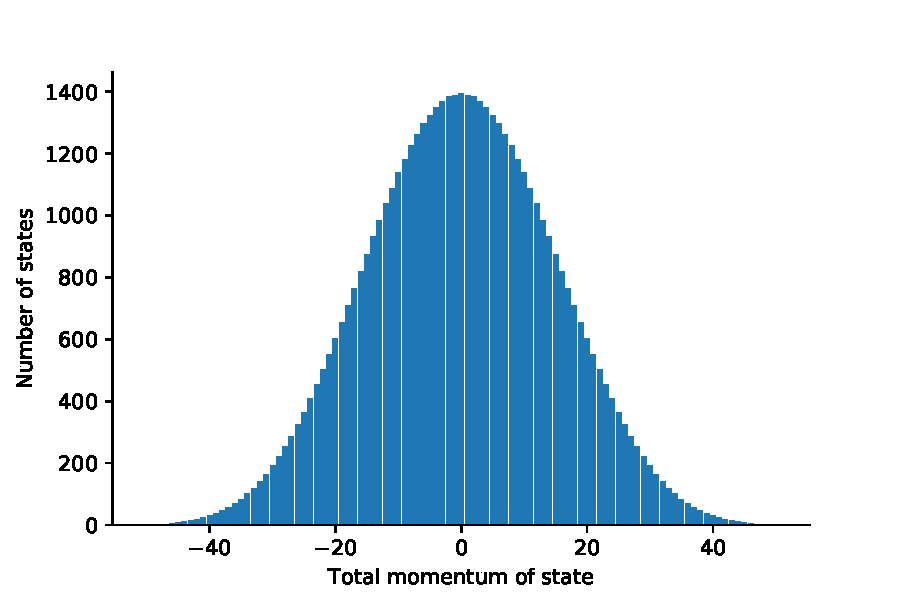
\includegraphics[width=0.7\textwidth]{no_of_states}
  \caption{The number of states in each momentum slice for the Lieb-Liniger model for \(N=5\) and \(I_{\max}=12\). Note that we dropped the prefactor \(\frac{2\pi}{L}\) for each entry.}
  \label{fig:no_of_states}
\end{figure}
The maximum possible state momentum is given by
\begin{align}
  \label{eq:50}
  P_{\max} = \frac{2\pi}{L}\sum_{i=0}^{N-1}(I_{\max}-i) = \frac{\pi}{L}N (2 I_{\max} -N +1) = \frac{\pi}{L}N (N_{\mathrm{world}} -N),
\end{align}
which in this case is \(\frac{L}{2\pi}P_{\max} = 35\).
We see however that if we calculate the sum rule saturations for each momentum slice, the saturations quickly go to 0 as \(\frac{L}{2\pi}P\) becomes larger (\cref{fig:saturationsperslice}), falling off especially for \(\abs{\frac{L}{2\pi}P}>I_{\max}\).
This is caused by the lack of states with larger momentum and proves especially problematic if we calculate total sum rule saturations over all states.
The higher momentum slices will suppress the total possible attainable sum rule.
\begin{figure}[tb!]
  \centering
   \subfloat{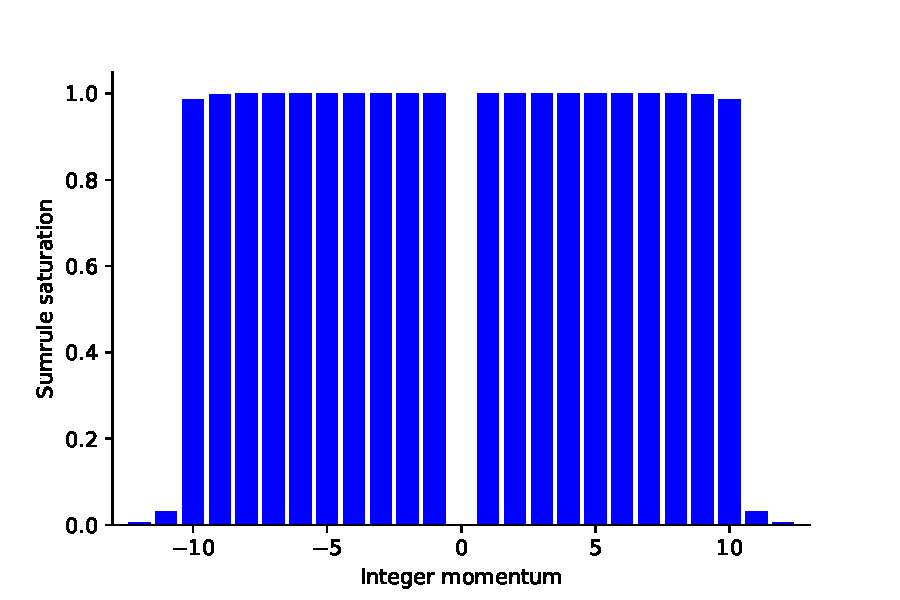
\includegraphics[width=.7\textwidth]{saturations_over_momenta.pdf}}
   \caption{Maximum possible sum rule saturation per momentum slice in the Hilbert space with \(I_{\max}=12\). Note how the saturations fall off sharply at around \(I_{\max}\). This is a result of the lack of states with the corresponding momentum. Not pictured are the saturations outside of the interval (-12,12), which decay exponentially.}
   \label{fig:saturationsperslice}
\end{figure}


The problem can be somewhat mitigated by giving \(I_{\max}\) two roles in the scanning.
It acts as both the cutoff for the momentum of individual particles as well as the total allowed momentum.
This contrasts with ABACUS, where \(I_{\max}\) acts only as the cutoff for the total momentum, meaning that states could in principle be built from particles with momentum far in excess of \(I_{\max}\), as long as particles with approximately opposite momentum cancel each other out.
Therefore ABACUS, when considering states, can always get high saturations in every momentum slice.
ABACUS also has the advantage that it can scan within a individual slice.
Due to this when calculating the f-sum rule saturation we only consider states for which \(\frac{L}{2\pi}P \in [-I_{\max},I_{\max}]\).
If we take all states in this interval and use \(N = 5\), \(I_{\max}=12\) the total sum rule saturation is approximately 83.5\%.

Furthermore we look at sum rule and form factor contributions for states with different number of particle-hole excitations, as calculated with~\cref{eq:52}.
Looking at \cref{fig:meanffphpairs}, where we plot the mean form factor sizes for each possible number of particle-hole pairs, we see that it decreases exponentially as \(N_{\mathrm{ph}}\) increases.
\begin{figure}[tb!]
  \centering
  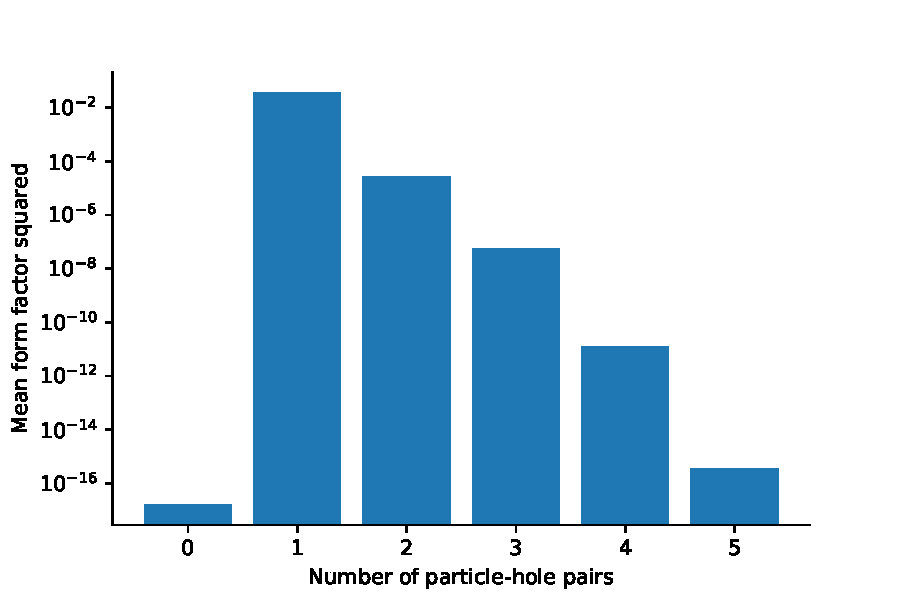
\includegraphics[width=.7\textwidth]{ave_form_factor_ph_pairs.pdf}
  \caption{Mean form factor per number of particle-hole pairs.}
  \label{fig:meanffphpairs}
\end{figure}

We see the same pattern of exponential decay when plotting the mean sum rule saturation per \(N_{\mathrm{ph}}\) (\cref{fig:meansumrulesaturation}). 
\begin{figure}[tb!]
  \centering
  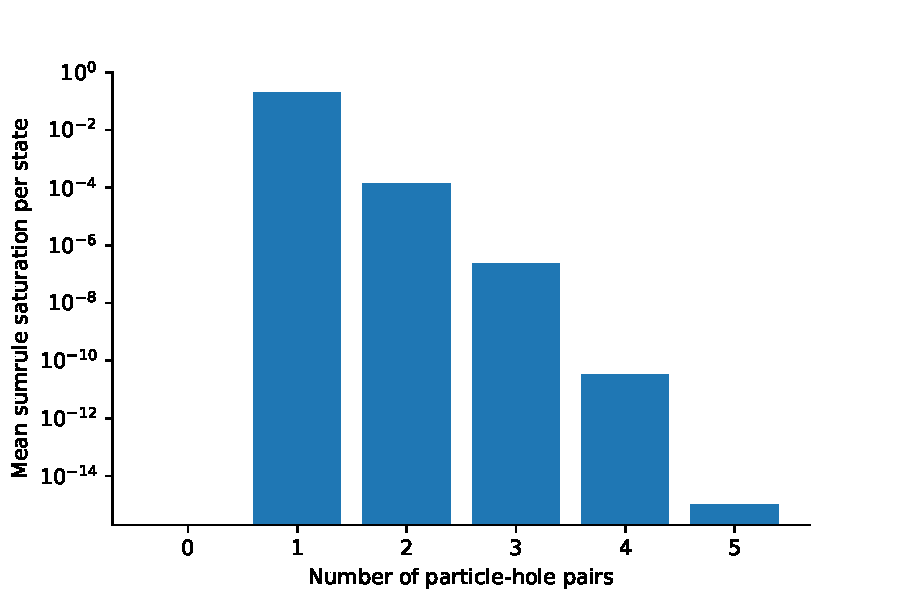
\includegraphics[width=.7\textwidth]{ave_sum_rule_saturation_ph_pairs.pdf}
  \caption{Mean sum rule saturation per given number of particle-hole pairs.}
  \label{fig:meansumrulesaturation}
\end{figure}

Even though the number of states with a given \(N_{\mathrm{ph}}\) increases for increasing \(N_{\mathrm{ph}}\), this only happens approximately linearly (\cref{fig:numberofstatesph}), meaning that only the states with \(N_{\mathrm{ph}}=1,2\) have a large contribution.
This validates the use of \cref{eq:52} while training to select for states with large matrix elements.
\begin{figure}[tb!]
  \centering
  \subfloat{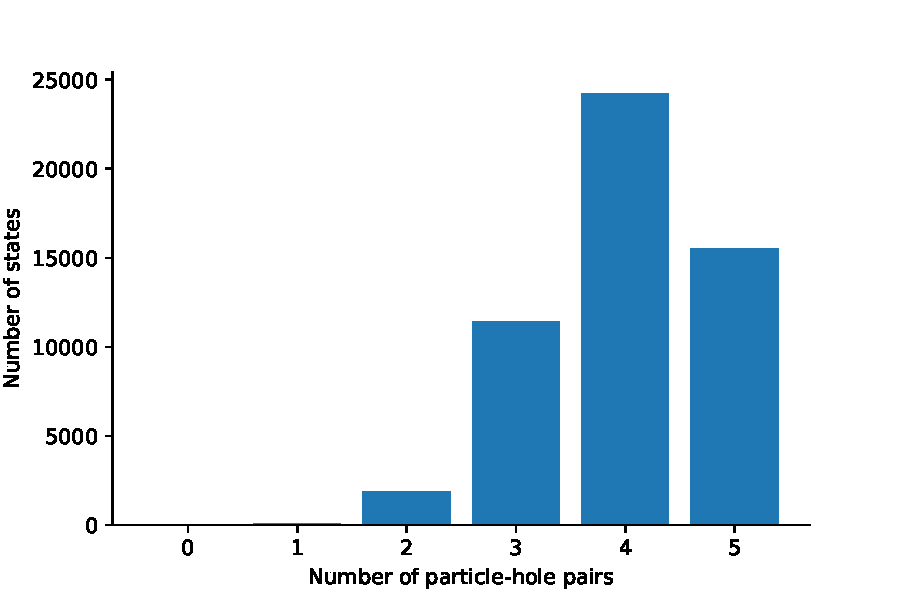
\includegraphics[width=.7\textwidth]{no_states_ph_pairs.pdf}}
  \caption{Number of states with a given number of particle-hole pairs.}
  \label{fig:numberofstatesph}
\end{figure}




\subsection{Numerical results}


We consider a number of different possible ways of determining states:
\begin{itemize}
\item A neural network trained with and without checking the number of particle hole pairs for states;
\item Random state selection. In this case we simply set \(\epsilon=1\) in the epsilon greedy algorithm and do not decrease it over the course of the run.
\end{itemize}
For both methods we calculate the DSFs both with and without minimizing \(N_{\mathrm{ph}}\).
The measure we use to compare methods is how many states are required to reach a given f-sum rule saturation.
Due to the representation of the states and the cutoff used, direct comparison with ABACUS is difficult (\cref{sec:exact}), but we do give some results for a rough estimate of relative performance.

Required sum rule saturation is set at 83\%, which in the given subspace corresponds to approximately \(83/83.5\approx99.5\%\) (\cref{sec:exact}).
We average the number of states necessary over 5 runs with random initial seed.
If training occurs we do so for 25 epochs of 500 states.
We set \(\epsilon=0.1\) and do not change it during training.
We do not start from full exploration (\(\epsilon=1\)) because many states will contribute very little to sum rule saturations, leading to poor results.
In evaluation we also have \(\epsilon=0.1\).
We set the hyperparameters \(\alpha=0.1\) and \(\gamma = 0.975\).
If convergence has not been reached after 3000 states, the scanning is terminated.
Encountered states are stored for later analysis as well as to prevent double counting.

As an approximate measure of the average size of matrix elements, we consider a linear trend line trough the data.
The value of the base offset acts as a proxy for the average size, allowing for a comparison between different methods.

For the reward function we do not use the obvious choice of form factors or sum rule saturation, since these measures span many decades.
Instead we use
\begin{algorithm}[H]
   \hspace*{\algorithmicindent} \textbf{Input} $\mathcal{F}, \mu, \lambda, N_{\mathrm{world}}$ 
   \begin{algorithmic}[1]
     \If{$\abs{\mathcal{F}}>10^{-5}$} 
     \State \Return $\abs{\mathcal{F}}^{1/10}$
     \ElsIf{$d(\mu, \lambda)<\sqrt{N_{\mathrm{world}}}$} 
     \State \Return $\sqrt{d(\mu, \lambda)}$
     \Else{}
     \State \Return -1
     \EndIf{}
  \end{algorithmic}
\end{algorithm}
\noindent
where \(\mathcal{F}\) is the form factor of the current state \(\mu\), \(\lambda\) is the reference state and \(d(\mu, \lambda)\) is the distance between the current state and the reference state, defines as
\begin{algorithm}[H]
   \hspace*{\algorithmicindent} \textbf{Input} $\mu, \lambda$ 
   \begin{algorithmic}[1]
     \State $d = 0$
     \For{$i$ such that $J(I_{\mu})_{I_i=1}$}
     \State $d = d + \abs{i - \left[J(I_{\lambda})_{I_j=1}\right]_i}$
     \EndFor{}
     \State \Return $d$
  \end{algorithmic}
\end{algorithm}
\noindent
with \(J\) an index set.
In other words, it is the distance each particle has traveled in Bethe number space from its original position in the reference state.



\begin{figure}[tb!]
  \centering
  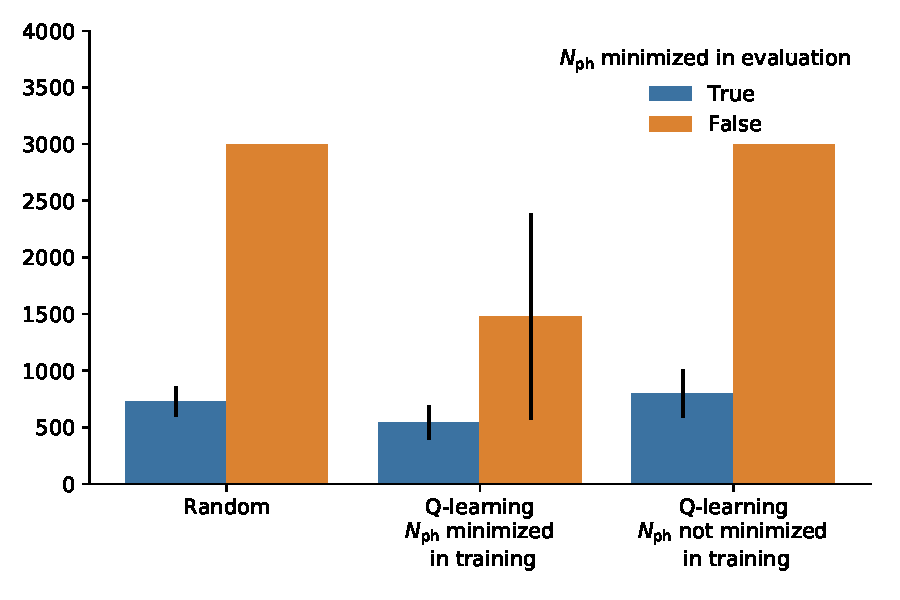
\includegraphics[width=0.7\textwidth]{statestoconv.pdf}
  \caption{Number of states needed to reach 83\% sum rule saturation averaged over five runs. The error bars denote standard errors.}
  \label{fig:statestoconv}
\end{figure}

\begin{figure}[tb!]
  \centering
  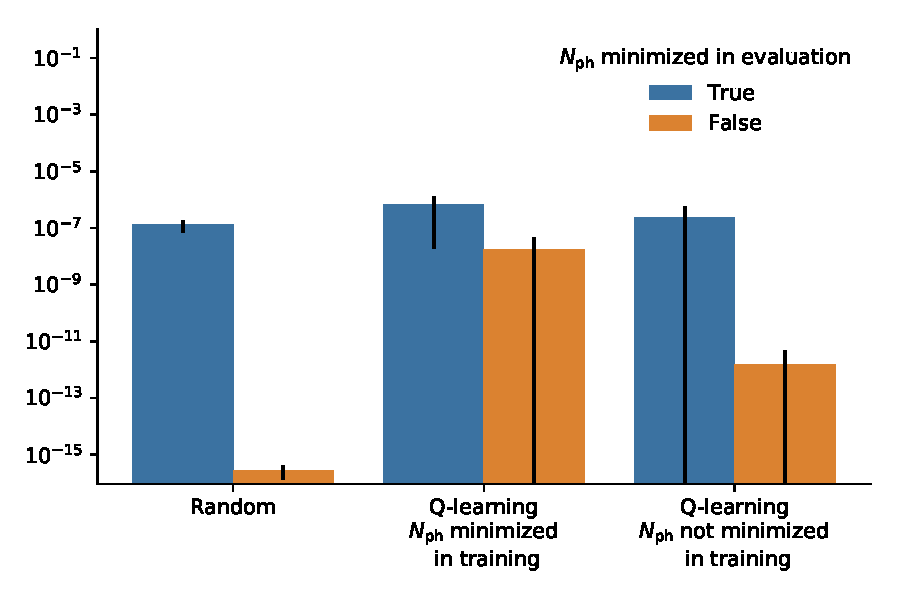
\includegraphics[width=0.7\textwidth]{ffsizesproxy.pdf}
  \caption{Mean square form factor size proxy average over five runs. The error bars denote standard errors.}
  \label{fig:ffsizeproxy}
\end{figure}


\Cref{fig:statestoconv} and \cref{fig:ffsizeproxy} show the results.
We consider states with \(c=1\), \(L=N=5\) and \(I_{\max}=12\).
Full results are found in \cref{chap:qlearningresults}.
The baseline measurement we use is a random exploration of the state space, with no checks on the number of particle-hole pairs during DSF calculation.
As long as an action is valid, meaning it does not add or remove particles where that is not possible, revisit a state or create a state with too large a momentum.
Looking at \cref{fig:saturation_rand_True_check_train_False_check_eval_False} we see that none of the runs converge after 3000 steps.
Average square form factor sizes are of order \(10^{-16}\), as seen in \cref{fig:ff_sizes_rand_True_check_train_False_check_eval_False}.

\begin{figure}[tb!]
  \centering
  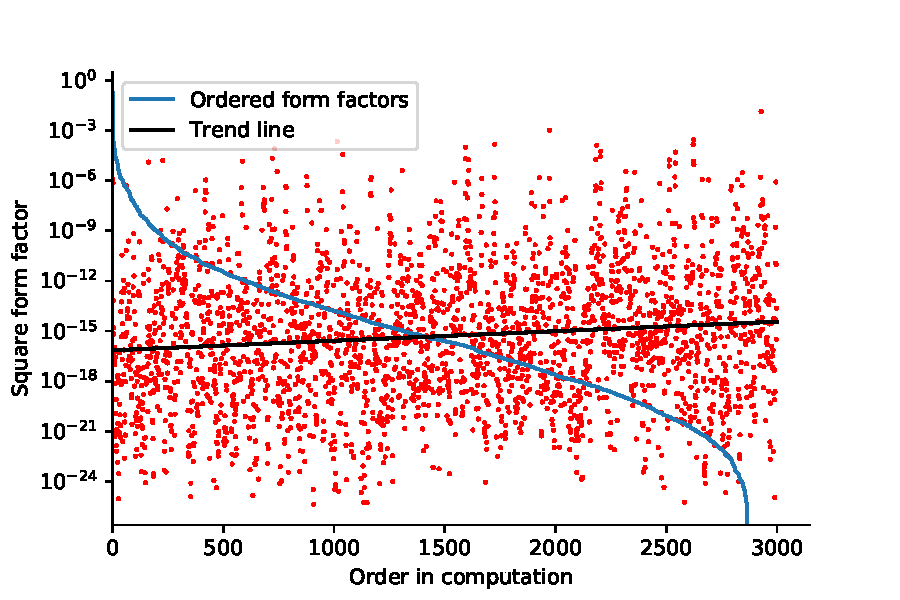
\includegraphics[width=0.7\textwidth]{ff_sizes_rand_True_check_train_False_check_eval_False.pdf}
  \caption{Square form factors as a function of order of computation for random state selection without minimizing \(N_{\mathrm{ph}}\) for a selected DSF calculation.}
  \label{fig:ff_sizes_rand_True_check_train_False_check_eval_False}
\end{figure}

\begin{figure}[tb!]
  \centering
  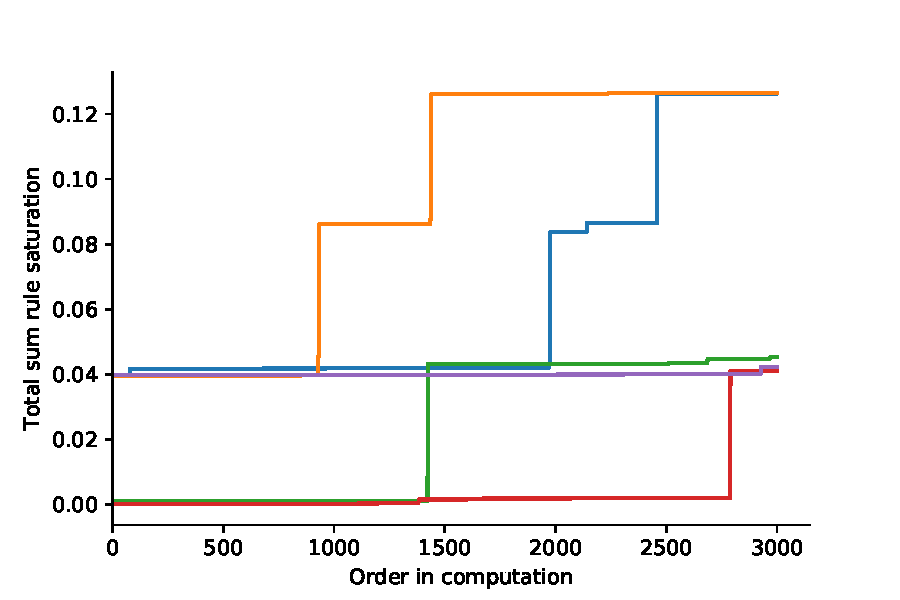
\includegraphics[width=0.7\textwidth]{saturation_histories_rand_True_check_train_False_check_eval_False.pdf}
  \caption{Saturation as a function of order of computation for random state selection without minimizing \(N_{\mathrm{ph}}\) for 5 runs of DSF calculation.}
  \label{fig:saturation_rand_True_check_train_False_check_eval_False}
\end{figure}

If we enforce particle-hole pair minimization, the picture changes.
Now only approximately 700 states are necessary to reach saturation, and average form factor size is of order \(10^{-6}\) (\cref{fig:ff_sizes_rand_True_check_train_False_check_eval_False}).
The source of randomness here is the random selection of the state with the lowest \(N_{\mathrm{ph}}\) from all states with the same value for \(N_{\mathrm{ph}}\).
We see that enforcing particle-hole minimization is an important measure in selecting states with large form factors.
Note the plateauing of the sum rule saturation that occurs for many runs (\cref{fig:saturation_rand_True_check_train_False_check_eval_False}). 
This probably happens because most of the large form factors have already been selected and the last few percentage points have to be made up by many form factors with small contributions.

\begin{figure}[tb!]
  \centering
  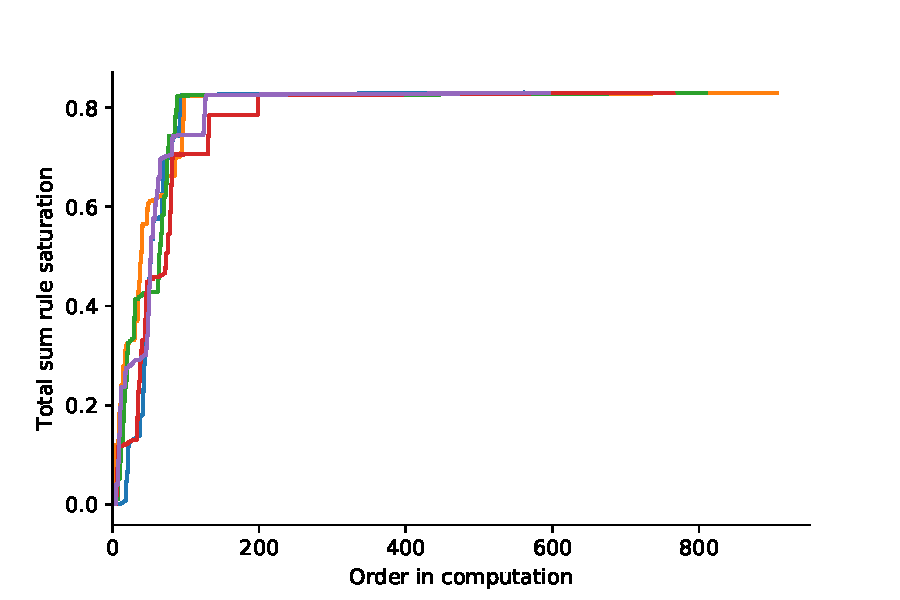
\includegraphics[width=0.7\textwidth]{saturation_histories_rand_True_check_train_False_check_eval_True.pdf}
  \caption{Saturation as a function of order of computation for random state selection while minimizing \(N_{\mathrm{ph}}\) for 5 runs of DSF calculation.}
\end{figure}

\begin{figure}[tb!]
  \centering
  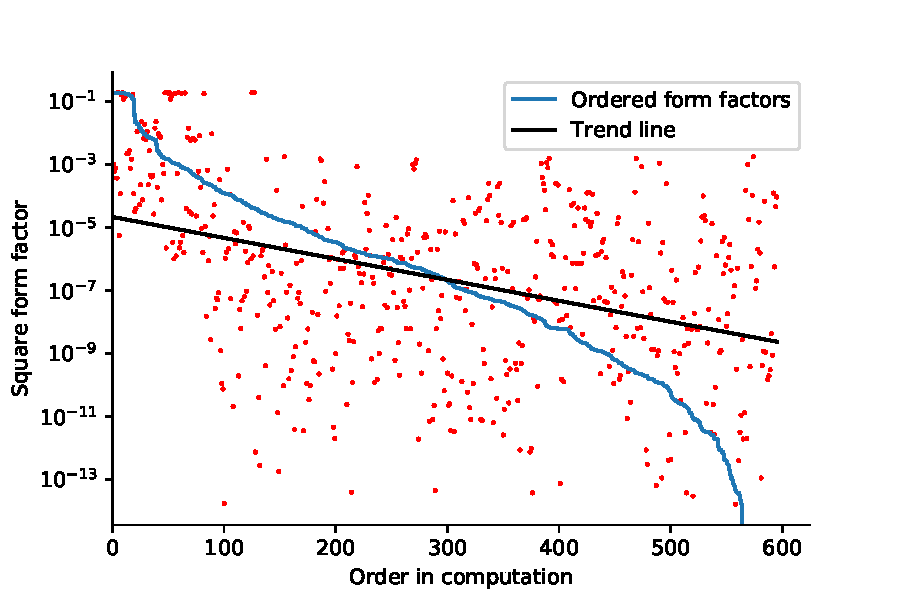
\includegraphics[width=0.7\textwidth]{ff_sizes_rand_True_check_train_False_check_eval_True.pdf}
  \caption{Square form factors as a function of order of computation for random state selection while minimizing \(N_{\mathrm{ph}}\) for a selected DSF calculation.}
\end{figure}

Now we come to the results of using Q-learning.
If \(N_{\mathrm{ph}}\)-minimization is used during both training and DSF calculation, we see the best results of all methods considered, with an average number of states to convergence of 630 (although again we often see a plateauing, \cref{fig:saturation_histories_rand_False_check_train_True_check_eval_True}).
The average form factor also has the largest value at order $10^{-5}$, although the error is large (\cref{fig:ff_sizes_rand_False_check_train_True_check_eval_True}).


\begin{figure}[tb!]
  \centering
  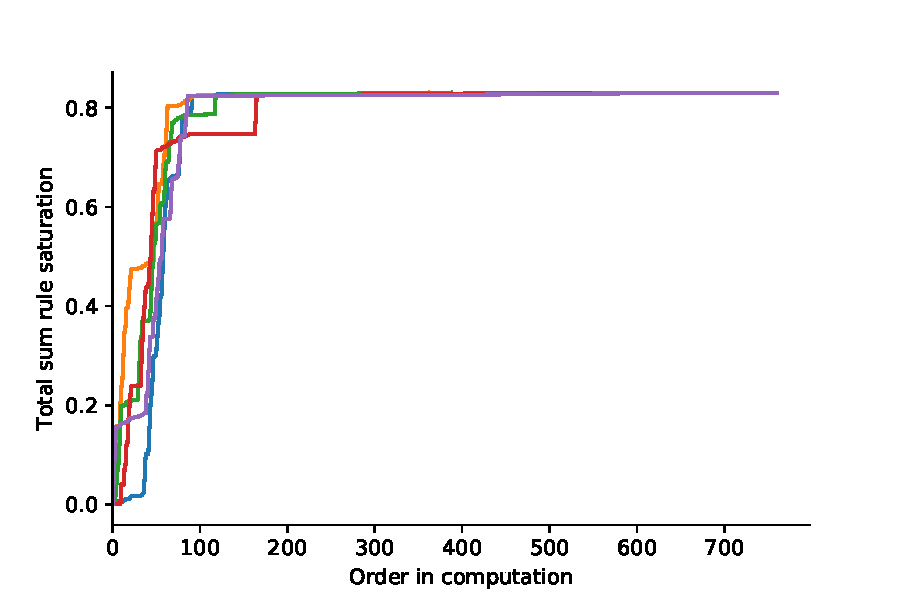
\includegraphics[width=0.7\textwidth]{saturation_histories_rand_False_check_train_True_check_eval_True.pdf}
  \caption{Saturation as a function of order of computation for Q-learning state selection while minimizing \(N_{\mathrm{ph}}\) during both training and DSF calculation, for 5 runs of DSF calculation.}
  \label{fig:saturation_histories_rand_False_check_train_True_check_eval_True}
\end{figure}

\begin{figure}[tb!]
  \centering
  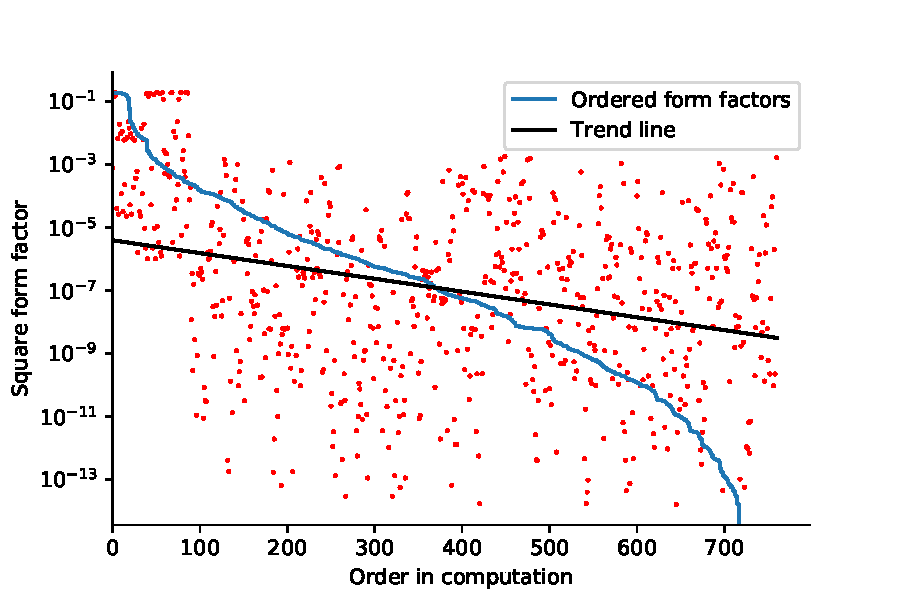
\includegraphics[width=0.7\textwidth]{ff_sizes_rand_False_check_train_True_check_eval_True.pdf}
  \caption{Square form factors as a function of order of computation for Q-learning state selection while minimizing \(N_{\mathrm{ph}}\) during both training and DSF calculation, for a selected DSF calculation.}
  \label{fig:ff_sizes_rand_False_check_train_True_check_eval_True}
\end{figure}

The most interesting result is seen when we do enable \(N_{\mathrm{ph}}\)-minimization during training but not during evaluation.
In this case the number of states required to reach saturation is 2081, although a large error of 483 states is present and one of the runs did not saturate after 3000 states (\cref{fig:saturation_histories_rand_False_check_train_True_check_eval_False}).
Average form factors are of order \(10^{-8}\) and visually comparing the results of this run (\cref{fig:ff_sizes_rand_False_check_train_True_check_eval_False}) with those of the random evaluation without \(N_{\mathrm{ph}}\)-minimization (\cref{fig:ff_sizes_rand_True_check_train_False_check_eval_False}) confirms this.
The performance of this method confirms that learning is occurring since there is no \(N_{\mathrm{ph}}\)-minimization occurring during evaluation, meaning that all decisions are based on the information present during training.


\begin{figure}[tb!]
  \centering
  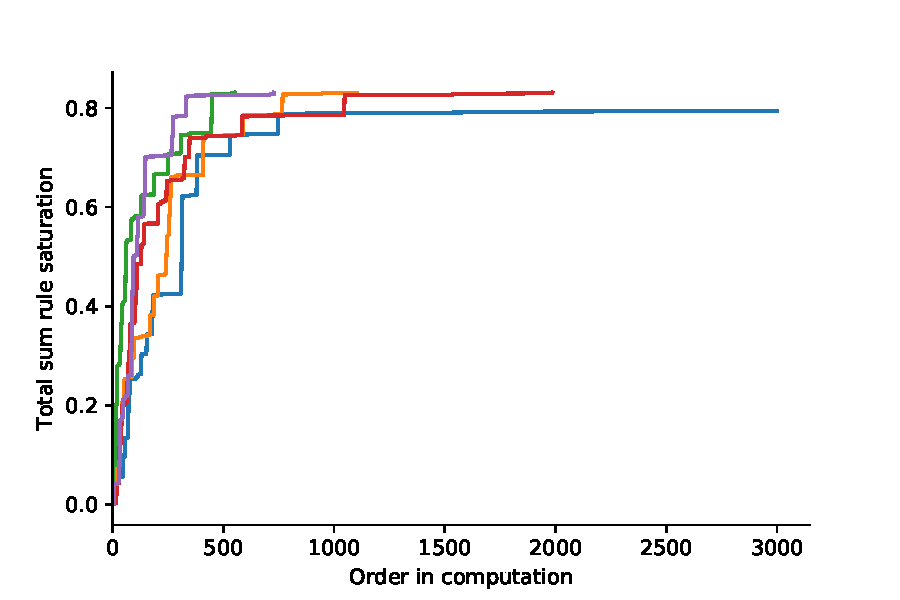
\includegraphics[width=0.7\textwidth]{saturation_histories_rand_False_check_train_True_check_eval_False}
  \caption{Saturation as a function of order of computation for Q-learning state selection while minimizing \(N_{\mathrm{ph}}\) during training but not during DSF calculation, for 5 runs of DSF calculation. Note that one of the DSF calculation runs did not converge, reaching $\sim79.5\%$ saturation after 3000 states.}
  \label{fig:saturation_histories_rand_False_check_train_True_check_eval_False}
\end{figure}

\begin{figure}[tb!]
  \centering
  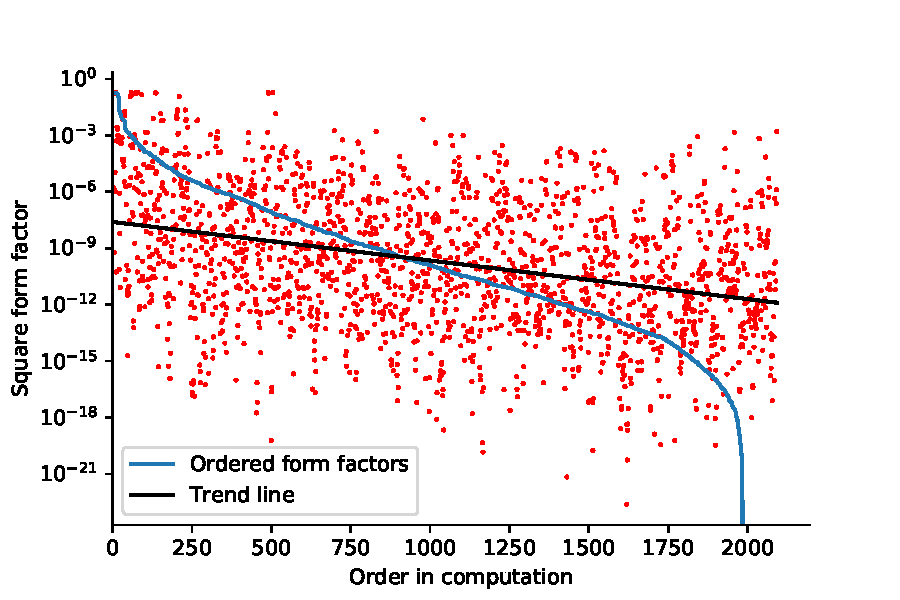
\includegraphics[width=0.7\textwidth]{ff_sizes_rand_False_check_train_True_check_eval_False.pdf}
  \caption{Square form factors as a function of order of computation for Q-learning state selection while minimizing \(N_{\mathrm{ph}}\) during training but not during DSF calculation, for a selected DSF calculation.}
  \label{fig:ff_sizes_rand_False_check_train_True_check_eval_False}
\end{figure}

That these results come from learning is further confirmed when considering the evaluation with particle-hole minimization disabled in training and enabled in evaluation.
The average number of states required is 752 (\cref{fig:saturation_histories_rand_False_check_train_False_check_eval_True}), with matrix elements of order \(10^{-6}\) (\cref{fig:ff_sizes_rand_False_check_train_False_check_eval_True}).
This is worse than with \(N_{\mathrm{ph}}\)-minimization enabled in training, pointing to a possibility that the minimization leads the model to learn about states with large contributions and consequently high rewards.


\begin{figure}[tb!]
  \centering
  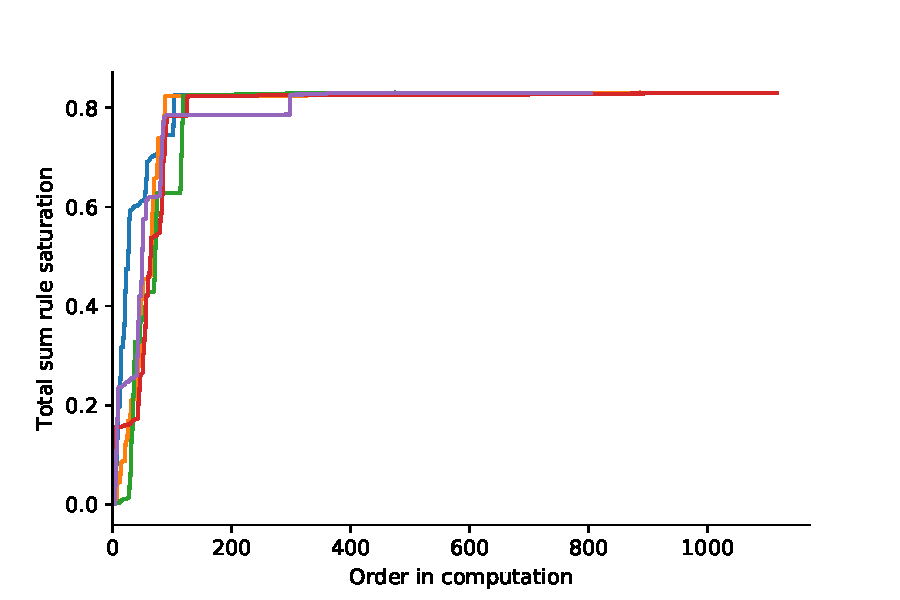
\includegraphics[width=0.7\textwidth]{saturation_histories_rand_False_check_train_False_check_eval_True.pdf}
  \caption{Saturation as a function of order of computation for Q-learning state selection while not minimizing \(N_{\mathrm{ph}}\) during training but with minimization during DSF calculation, for 5 runs of DSF calculation.}
  \label{fig:saturation_histories_rand_False_check_train_False_check_eval_True}
\end{figure}

\begin{figure}[tb!]
  \centering
  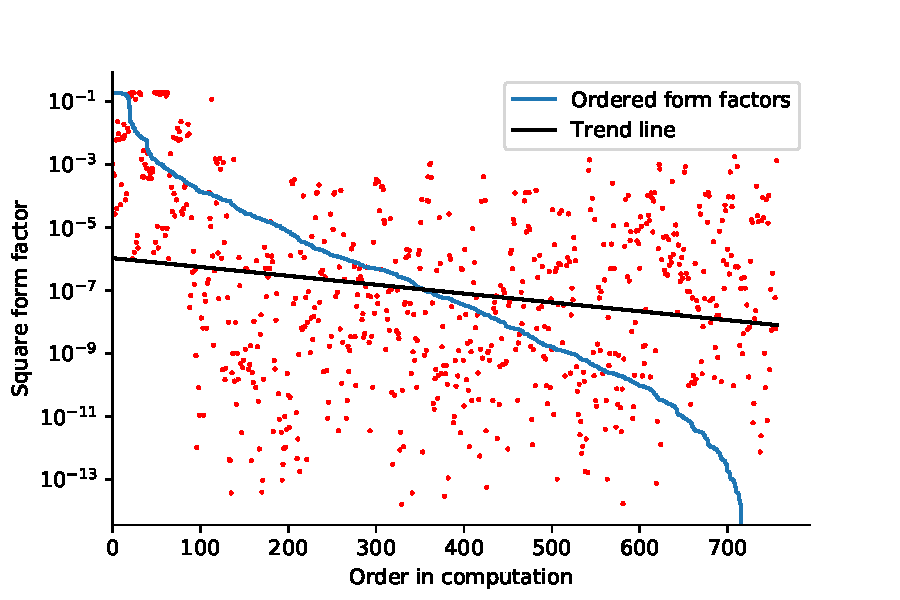
\includegraphics[width=0.7\textwidth]{ff_sizes_rand_False_check_train_False_check_eval_True.pdf}
  \caption{Square form factors as a function of order of computation for Q-learning state selection while not minimizing \(N_{\mathrm{ph}}\) during training but with minimization during DSF calculation, for a selected DSF calculation.}
  \label{fig:ff_sizes_rand_False_check_train_False_check_eval_True}
\end{figure}

Finally we come to an evaluation with \(N_{\mathrm{ph}}\)-minimization disabled in both training and evaluation.
Here none of the five runs converge (\cref{fig:saturation_histories_rand_False_check_train_False_check_eval_False}) and the average form factor is of order \(10^{-15}\) (\cref{fig:ff_sizes_rand_False_check_train_False_check_eval_False}).
The poor results of this method shows that using only the reward function to shape action selection does not provide enough feedback for learning.

\begin{figure}[tb!]
  \centering
  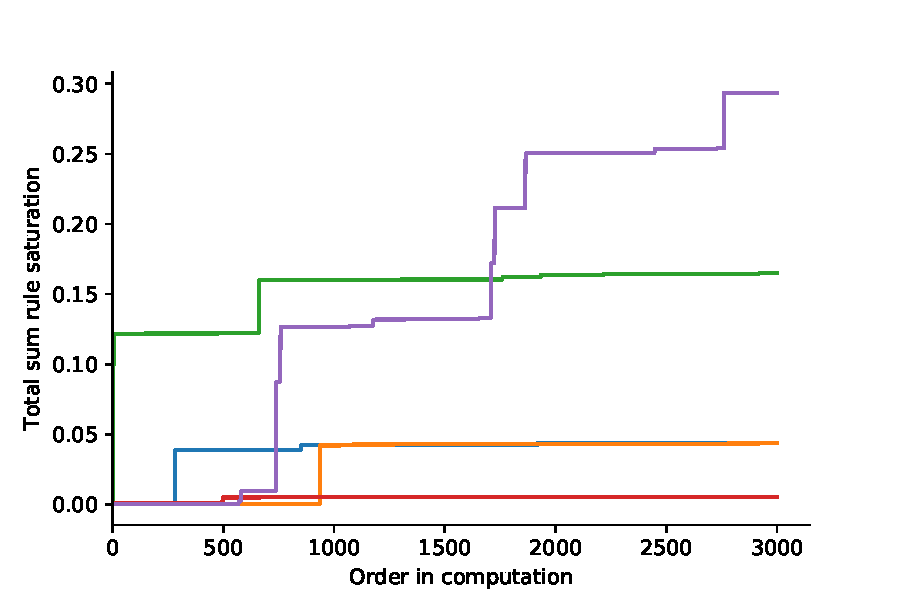
\includegraphics[width=0.7\textwidth]{saturation_histories_rand_False_check_train_False_check_eval_False.pdf}
  \caption{Saturation as a function of order of computation for Q-learning state selection without minimizing \(N_{\mathrm{ph}}\) during either training and DSF calculation, for 5 runs of DSF calculation.}
  \label{fig:saturation_histories_rand_False_check_train_False_check_eval_False}
\end{figure}

\begin{figure}[tb!]
  \centering
  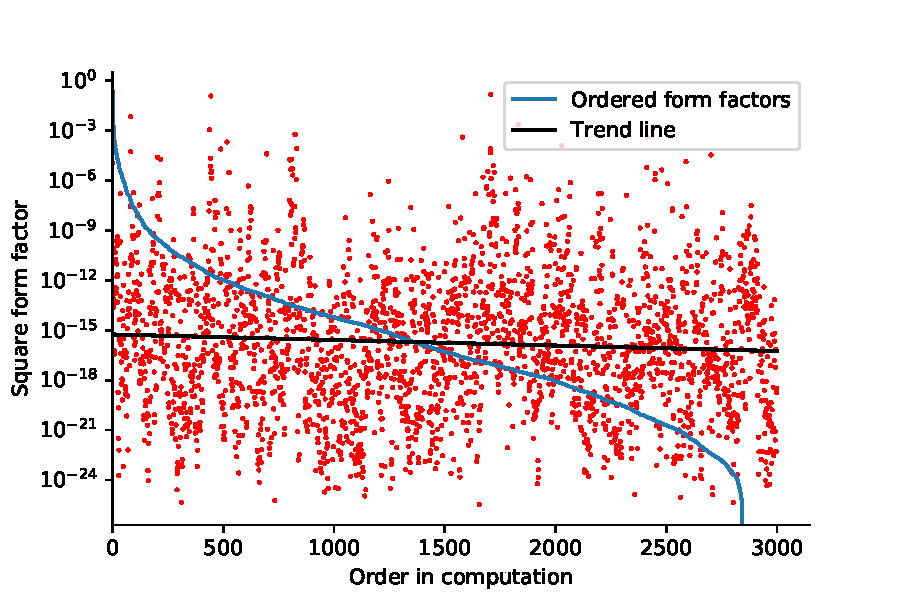
\includegraphics[width=0.7\textwidth]{ff_sizes_rand_False_check_train_False_check_eval_False.pdf}
  \caption{Square form factors as a function of order of computation for Q-learning state selection without minimizing \(N_{\mathrm{ph}}\) during either training and DSF calculation, for a selected DSF calculation.}
  \label{fig:ff_sizes_rand_False_check_train_False_check_eval_False}
\end{figure}

An illustration of the learned behaviour is visible when considering the trained model of the Q-function of a system with \(N=11\) and \(I_{\max}=20\).
When evaluating the ground state (\cref{fig:binarygroundstate}), we clearly see a structure occurring in the resulting Q-matrix (\cref{fig:qmatrix}, top).
Unoccupied positions should not be selected for removal, while occupied positions should not be selected for particle placement.
We see this occurring in the form of bands of high and low Q-factors.
The horizontal yellow of high Q-factors band consists of actions that would take a particle from the Fermi interval and deposit it somewhere outside.
In contrast the vertical blue band corresponds to forbidden actions that would take a particle from an unoccupied position and place it on an already occupied site.
These actions with two forbidden sub-actions are more strongly disfavored than the actions represented by the corner quadrants, which represent taking a particle from an unoccupied position and placing it at another unoccupied site.
The band structures are clearer when we highlight the 100 lowest (\cref{fig:qmatrix}, lower left) and highest (\cref{fig:qmatrix}, lower right) Q-factors.

\begin{figure}[tb!]
  \centering
  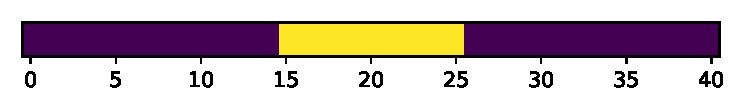
\includegraphics{state.pdf}
  \caption{Ground state of the Lieb-Liniger model in binary representation with \(N=11\) and \(I_{\max}=20\). The yellow dots represent particles.}
  \label{fig:binarygroundstate}
  \vspace*{\floatsep}
  \subfloat{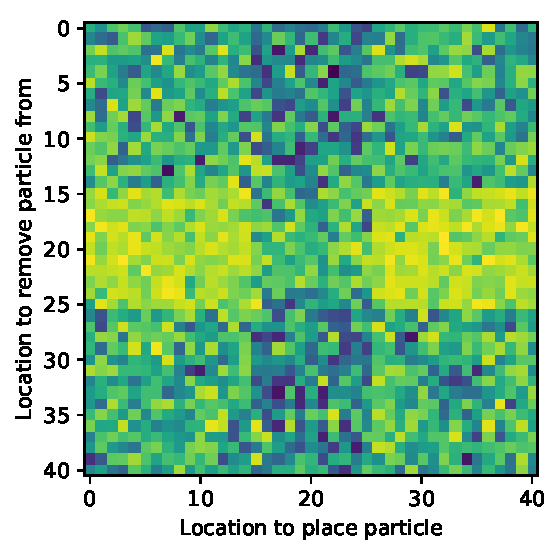
\includegraphics[width=.5\textwidth]{q_function_no_highlight.pdf}}\\
  \subfloat{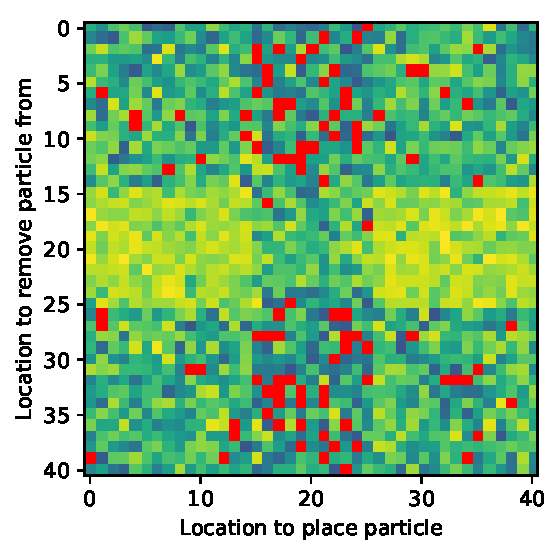
\includegraphics[width=.5\textwidth]{q_function_worst_highlighted.pdf}}
  \subfloat{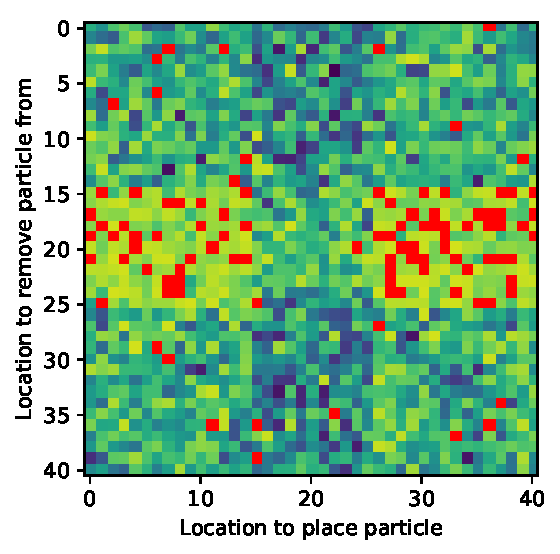
\includegraphics[width=.5\textwidth]{q_function_best_highlighted.pdf}}
  \caption{Q-matrix for the Lieb-Liniger model ground state with \(N=11\) and \(I_{\max}=20\) (top). In the lower left image, the 100 lowest Q-factors are highlighted, while the 100 best are shown in the lower right image.}
  \label{fig:qmatrix}
\end{figure}


Finally, we compare with ABACUS.
We calculate the density-density DSF for \(c=1\), \(L=N=11\) and \(I_{\max}=40\).
This yields a state space of size \(\binom{81}{11}\approx 1.2\times 10^{13}\).
The desired sum rule saturation of 99.9\% (\cref{fig:abacus_saturations}) is achieved with 9376 states, summed over approximately 7 seconds.
This is at most a fraction \(7.7\times 10^{-10}\) of the Hilbert space under consideration.
The form factor size proxy has a value of \num{8.01e-05} (\cref{fig:abacusformfactors})
This shows that ABACUS is highly efficient in summing matrix elements.

In conclusion we can say that learning does occur when using Q-learning to sum matrix elements, but that this method is far outclassed by the current implementation of ABACUS.
Of special note is the speed at which ABACUS operates, summing 10000 states in 7 seconds, while evaluation of approximately 2000 states takes 20 seconds, preceded by 600 seconds of training.


\begin{figure}[tb!]
  \centering
  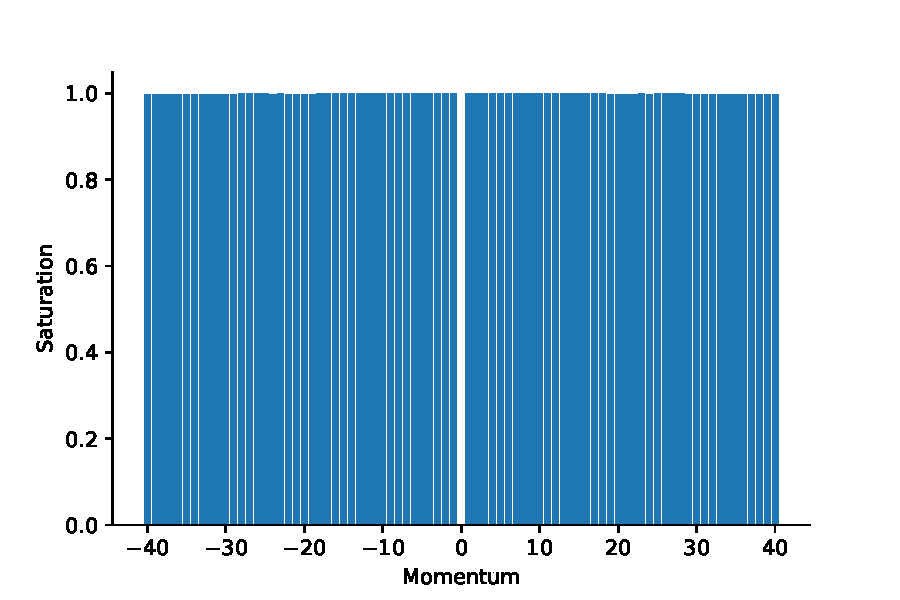
\includegraphics[width=0.7\textwidth]{abacus_saturations.pdf}
  \caption{Saturation per momentum slice for the density operator of the Lieb-Liniger model, at \(c=1\), \(L=N=11\), \(I_{\max}=40\), calculated with ABACUS.}
  \label{fig:abacus_saturations}
\end{figure}

\begin{figure}[tb!]
  \centering
  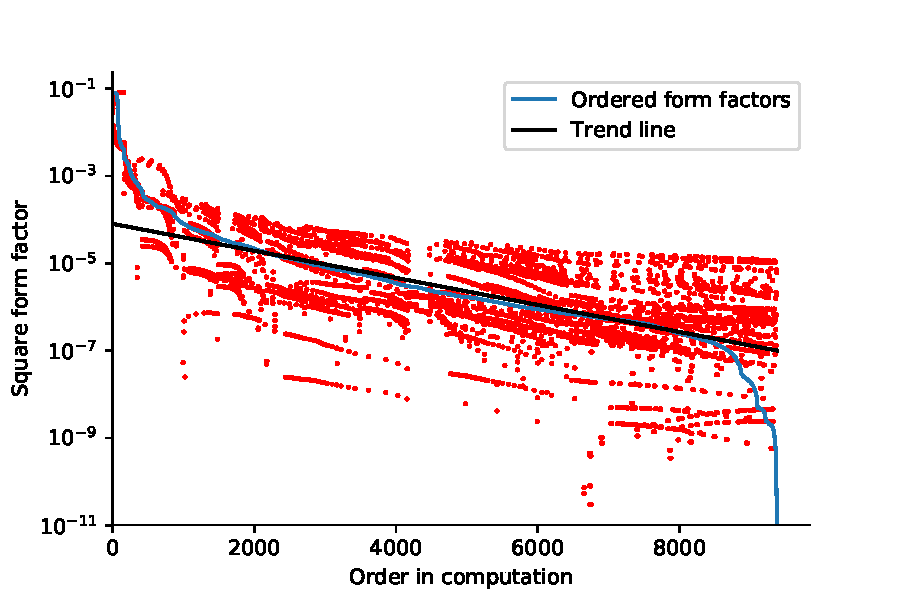
\includegraphics[width=0.7\textwidth]{abacus_ff_sq.pdf}
  \caption{Squared form factor for the density operator of the Lieb-Liniger model, at \(c=1\), \(L=N=11\), \(I_{\max}=40\), calculated with ABACUS.}
  \label{fig:abacusformfactors}
\end{figure}







\begin{savequote}[50mm]
I may not have gone where I intended to go, but I think I have ended up where I needed to be.
\qauthor{Douglas Adams, The Long Dark Tea-Time of the Soul}
\end{savequote}



\chapter{Discussion and conclusion}\label{chap:conclusion}


\section{Discussion}

A number of difficulties may be identified with the results mentioned.

\subsection{Non-Markovian nature of DSF Hilbert scanning}

Firstly, while the Lieb-Liniger model is Markovian, the Hilbert space scanning used to calculate DSFs is not.
This is because, to prevent overcounting, the entire history of previously visited states must be taken into consideration during each state selection.



Does this mostly have to do with the proofs of convergence just becoming easier when considering Markovian problems?


\cite{whitehead95_reinf_learn_non_markov_decis_proces}

\subsection{Problems with reinforcement learning}


There are also a number of issues with reinforcement learning more generally.
On of those is that reinforcement learning is data inefficient, sometimes extremely so.
In~\cite{1710.02298} a study was made of performance in the Atari learning environment by combining different techniques beyond those used in \cite{mnih13_playin_atari_with_deep_reinf_learn,mnih15_human_level_contr_throug_deep_reinf_learn}.
Even in the best case approximately 15 million frames (at 60 Hertz) were required to reach human-level performance, corresponding to 3 days of gametime.
This was however already an improvement on the original work done in~\cite{mnih15_human_level_contr_throug_deep_reinf_learn}, where only 1 in 4 frames where used to improve computational efficiency and which required 38 days of gametime to train on 50 million sample frames.
A similar data inefficiency is seen in~\cite{heess17_emerg_locom_behav_rich_envir}.
Although the results are impressive (an agent learns to navigate a challenging environment consisting of hurdles and gaps using only a simple reward function), training took 100 hours of wall clock time on 64 workers~\cite[Figure 1]{heess17_emerg_locom_behav_rich_envir}.

At the same time state of the art machine learning setups are experiencing an large increase in compute power used.
Data~\cite{amodei2018} compiled by the nonprofit OpenAI\footnote{OpenAI was founded with the goal of doing research in finding safe ways towards the realization of artificial general intelligence (see \href{https://openai.com/about/}{https://openai.com/about/}).} shows an increase of a factor 300000 in the number of petaflop/s-day\footnote{A petaflop/s-day is defined as doing $10^{15}$ neural network operations per second for one day, or approximately $10^{20}$ operations per day~\cite{amodei2018}.} used in training machine learning systems between 2012 and the end of 2017 (\cref{fig:increasedaiflops}). 
This corresponds to a doubling time of 3.5 months and is mostly the result of increased parallelism and monetary investments.
This is far in excess of the doubling time of 18 to 24 months predicted by Moore's law.

\begin{figure}[tb!]
  \centering
  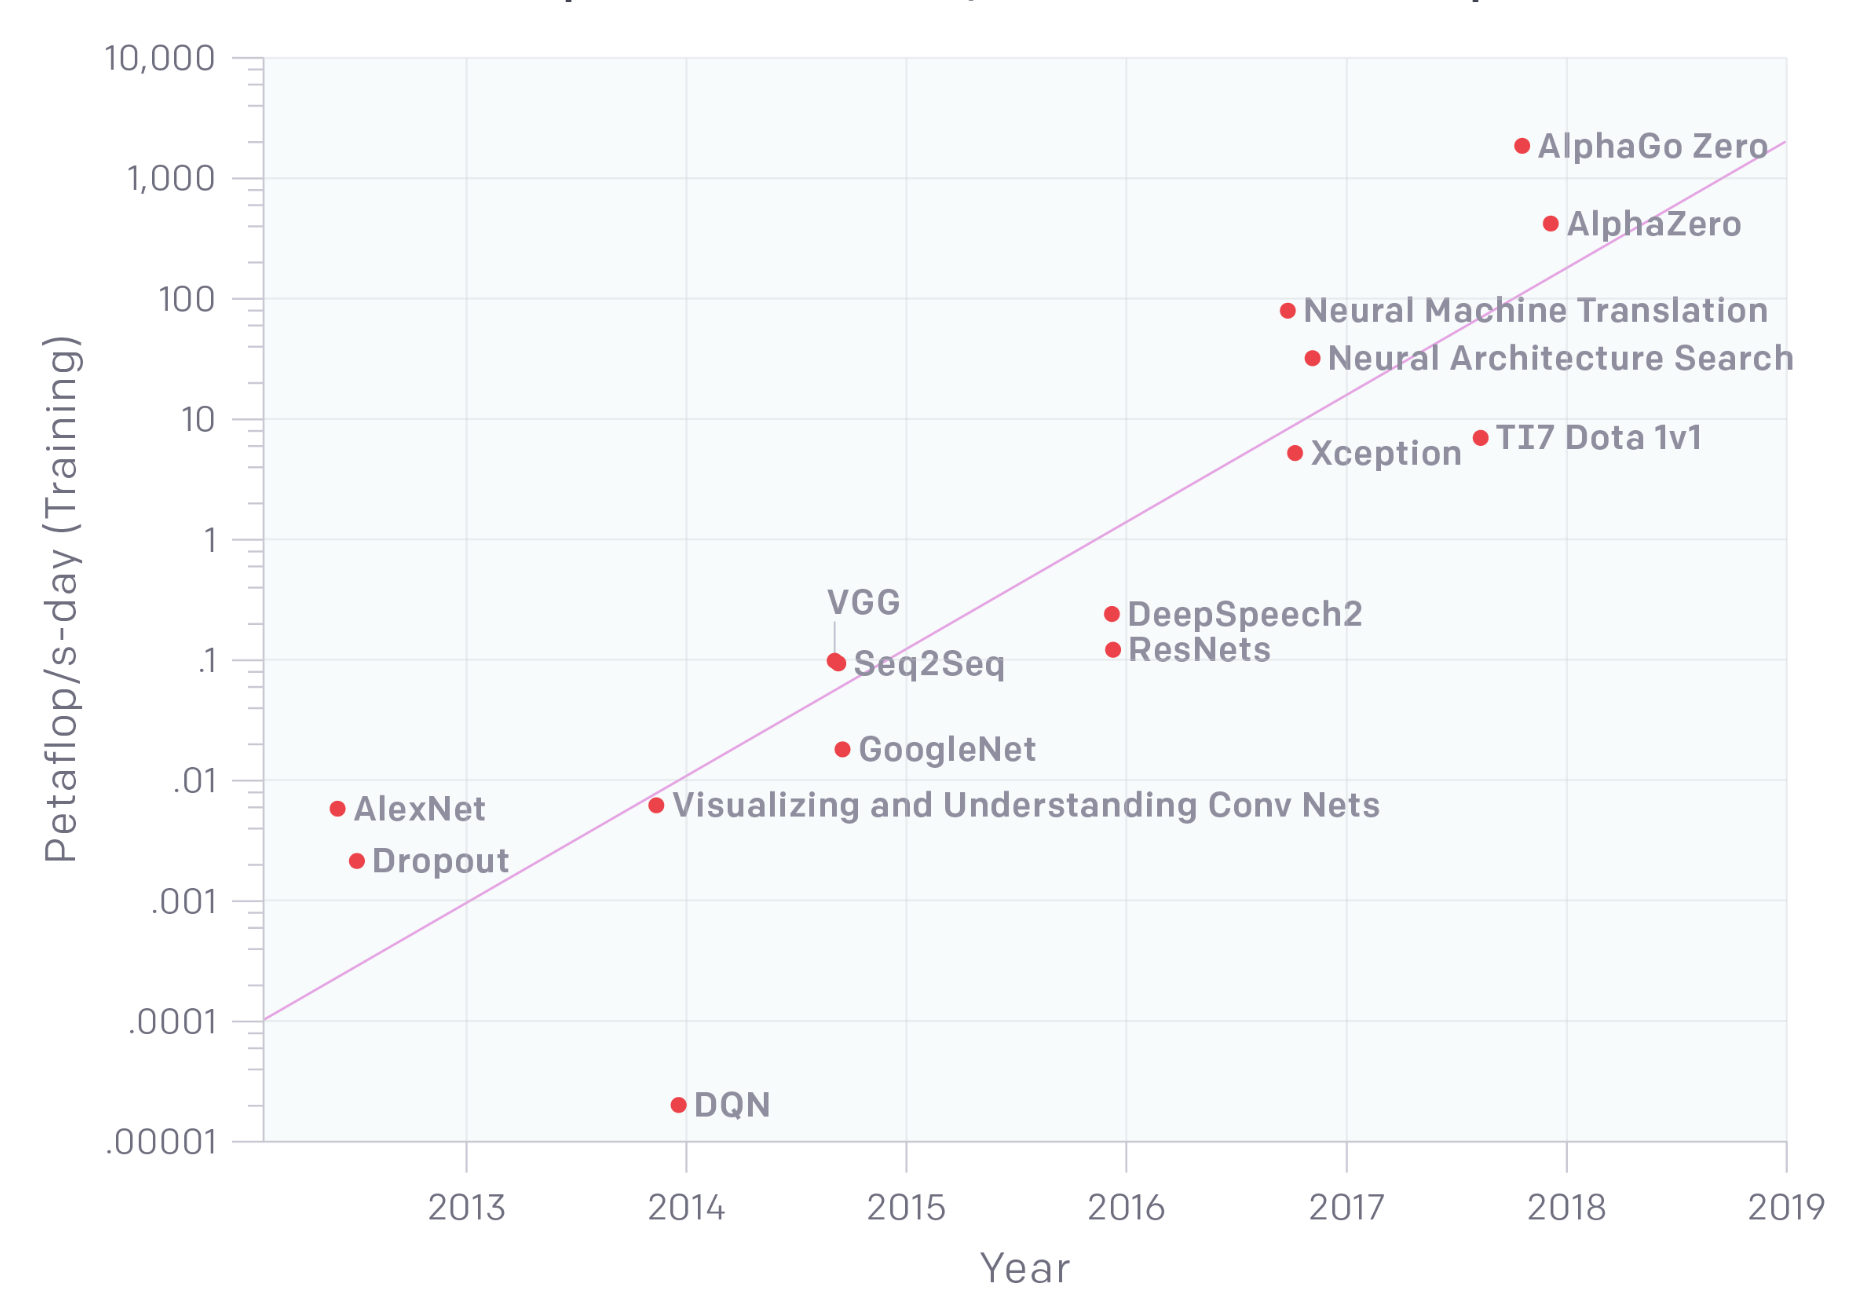
\includegraphics[width=0.7\textwidth]{increaseaiflops.png}
  \caption{Log plot of petaflop/s-day used in training AI over time. Doubling time is 3.5 months. Figure taken from~\cite{amodei2018}}
  \label{fig:increasedaiflops}
\end{figure}

Another difficulty more specific to reinforcement learning and evolutionary computing is the design of reward functions.
Reward function are often designed to provide a simple quantitative measure which corresponds to the desired goal.
The solutions with which algorithms come up are sometimes not in line with what researchers expect.

One example consisted of a simulated environment in which the goal was to evolve creatures that would evolve locomotive strategies, with fitness measured by the average ground velocity over 10 seconds.
Instead of developing movement strategies, some creatures would evolve to have a long rigid body, which would fall over when the simulation started, causing large average ground velocities.

Another example is seen in automated program repair, where a program fixes another buggy program automatically.
A set of tests is written which the program has to pass.
GenProg, which used digital evolution to generate debugging programs, fixed a sorting algorithm by always making it return an empty list, which the tests considered as sorted.

Solutions may also depend on bugs in the simulation platform being used, acting in a way as automated bug discovery.
In a simulation in which swimming strategies were evolved, the simulation used inaccurate numerical simulation.
Fast motion would lead to the accumulation of errors, which was exploited by creatures by twitching body parts rapidly, providing free energy.
In a similar vein buggy collision detection was used by creatures to obtain free energy by penetrating the ground.
When the simulation picked this up and corrected it, the upward force led to forward locomotion~\cite{1803.03453}.\footnote{Reference~\cite{1803.03453} contains many more examples.} 

Preventing such reward function hacking and undesired side effects is an emerging field of study within AI, foreshadowing the possible eventual emergence of artificial general intelligence~\cite{amodei16_concr_probl_ai_safet}.
Concurrently we are seeing a political debate develop related to the ways in which AI may be used maliciously~\cite{brundage18_malic_use_artif_intel}.

Reward function with a simple scoring also have difficulties when confronted with problems where there is a clear temporal structure.
An example of this can be found in the game Montezuma's revenge, in which a tomb is traversed in search of treasure.
This game has a temporal structure in that certain doors within the game are locked until the player retrieves the appropriate key.
A reward function based only on score performs poorly in this game~\cite{mnih15_human_level_contr_throug_deep_reinf_learn}, because it is not able to causally reason about the actions required to maximize score.

We also see this in the DSF scanning developed here.
The obvious choice for the reward function is the absolute form factor squared for the operator under consideration.
The problem with this approach comes from the many decades spanned by the form factors.
This makes the rewards for many transition very small, meaning it will often not even register as noise.

Finally machine learning research is currently facing problems with regards to reproducibility of findings.
This is caused by non-determinism in the research environment, for example by the effects different random seeds have on the weight initialization of models.
Different initializations may lead to large 


Reproducibility of RL solutions is often an issue~\cite{1709.06560}.
3.10. Deep learning thus far is difficult to engineer with \cite{marcus18_deep_learn}

Has plot with performance, performance 25th percentile is almost 0\cite{houthooft16_vime}
A visualization of this problem is seen in \cref{fig:halfcheetah}.\footnote{HalfCheetah is a research environment for reinforcement learning in which a cheetah like creature has the goal of learning to walk.}
\begin{figure}[tb!]
  \centering
  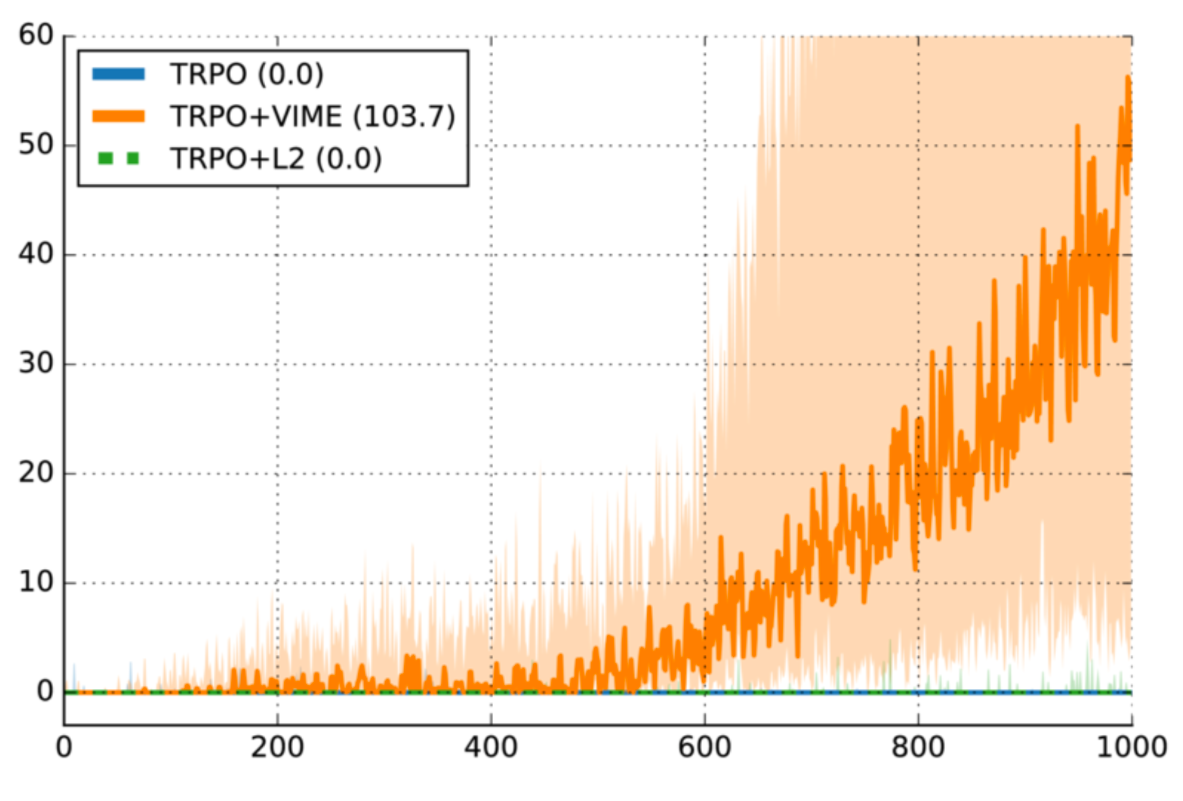
\includegraphics[width=0.7\textwidth]{rllearningtrouble.png}
  \caption{Taken from~\cite{houthooft16_vime}.}
  \label{fig:halfcheetah}
\end{figure}





\cite{marcus18_deep_learn}




\section{Conclusion}

Based on measurements the prediction of rapidities does not improve the calculation.

In general reinforcement learning is very data inefficient, leading to the conjecture that a well crafted function may work better in this domain.
As mentioned in~\cite{Caux2009} the applicability of ABACUS for large systems stems from the preliminary information provided by integrability, built into the algorithm.
We are seeing an increase in the system sizes realizable with exact diagonalization, with the low-energy properties of up to 50 spin-1/2 particles now accessible~\cite{wietek18_sublat_codin_algor_distr_memor}.

\subsection{Outlook}

The field of machine learning and artificial intelligence in general is currently experiencing large changes.

Reinforcement learning may also be used in rapidity determination.
Given a set of Bethe numbers, the rapidities can be predicted, after which convergence to machine precision is achieved through Newton iterations.
The number of iterations may be used as part of a reward function, with the goal to improve the rapidity predictions.

One of the limitations of the current approach of the system is that it requires a UV cutoff of the Bethe numbers in order to be able to represent possible moves in Hilbert space.
Since the size of the action space scales as \((I_{\infty+} + I_{\infty-} + 1)^2\) this means that action space sizes quickly become too large for efficient computation, irrespective of the number of particles involved.
A possible solution is the extension of the value function to a continuous domain.
This has recently been done in continuous control applications such as operating a simulated gripper to grab a ball, controlled only by applying torque to joints~\cite{lillicrap15_contin_contr_with_deep_reinf_learn,gu16_contin_deep_q_learn_with}.
Another improvement may come from using experience replay\cite{mnih15_human_level_contr_throug_deep_reinf_learn,mnih13_playin_atari_with_deep_reinf_learn}.
This allows for a way to deal with high correlation between consecutive states, by saving a tuple consisting of the current state, the action taken, the observed reward and the new state.
Training is then performed on mini-batches of this set of transitions.
This has the advantage that data is used multiple times during training, improving efficiency.
Furthermore the correlations between consecutive states are broken, reducing the variance of updates.
We did not use it here because in DSF calculation states may only be seen once to prevent double counting, thus making individual states not independent of the states that came before.

A weakness in the current implementation is that only ``connected states'' can be reached from any given state.
With this we mean states that differ only by a single particle move from the current state under consideration.
This differs from ABACUS, in which a tree of states is descended and at any point any previously reached state may be used as the base for a new expansion into Hilbert space.
The tree-like approach may be considered for further research.

Does this generalize to other models? It should, as long as you are able to find the DSFs you are interested in since you need them for the sum rule.

This may also generalize to models beyond the Lieb-Liniger model.
Since the scanning is model independent (only taking in the Bethe numbers of the model), as long as the f-sum rule for the desired DSF is known, we can optimize the state scanning.

\section*{Acknowledgements}
I would like to thank Jean-Sébastien Caux for his supervision and valuable suggestions.
Sam Kuypers is thanked for help in understanding some derivations.
I would also like to thank Sam, along with the rest of the J-S master gang (Jorran de Wit and Rebekka Koch), for providing a fun environment to work in and their willingness to hear me grumble about my project.
Once a Bethe bitch, always a Bethe bitch.

\appendix

\begin{savequote}[50mm]
If this goes badly and I make a crater, I want it named after me!
\qauthor{Iain M. Banks, Against a Dark Background}
\end{savequote}

\chapter{Boundary term of the Lieb-Liniger model}\label{cha:boundary}

Here we explicitly derive the boundary term (\cref{eq:lieblinigerboundary}) of the Lieb-Liniger model~\cite{Caux2015}.
We start with the Schrödinger equation
\begin{equation}
	\left[- \frac{\partial^2}{\partial x_1^2} - \frac{\partial^2}{\partial x_2^2} + 2c \delta(x_1 - x_2)\right] \psi(x_1, x_2) = E \psi(x_1,x_2).
\end{equation} 
Substituting \(x_+ = \frac{x_1+x_2}{2}\) and \(x_-=x_1-x_2\) this becomes
\begin{align}
  \label{eq:17}
  	\left[-\frac{1}{2}\frac{\partial^2}{\partial x_+^2} - 2\frac{\partial^2}{\partial x_-^2} + 2c \delta(x_-)\right] \psi = E\psi.
\end{align}
Integrating over an interval \(x_-\in[-\epsilon,\epsilon]\) we get
\begin{align}
  \label{eq:18}
  -\frac{1}{2} \frac{\partial^2}{\partial x_+^2} \int_{-\epsilon}^{\epsilon} \psi \dd x_- - 2 \int_{-\epsilon}^{\epsilon} \frac{\partial^2}{\partial x_-^2}\psi \dd x_- + 2c\int_{-\epsilon}^{\epsilon} \delta(x_-)\psi \dd x_- = E\int_{-\epsilon}^{\epsilon} \psi \dd x_.
\end{align}
The first term on the left hand side becomes 0 on \(\lim_{\epsilon\to0^+}\) as well as the term on the right hand side, leaving us with
\begin{align}
  \label{eq:19}
  \left.- \frac{\partial}{\partial x_-} \psi \right|_{x_-=-0^+}^{x_-=0^+}  + \left.c\psi\right|_{x_-=0} = 0.
\end{align}

Given that we are dealing with the bosonic case we require symmetric wave functions, \(\psi(x_1,x_2)=\psi(x_2,x_1)\).
This simplifies the result to
\begin{align}
  \label{eq:20}
  \left.(\partial_{x_2} - \partial_{x_1} - c) \psi(x_1, x_2)\right|_{x_2-x_1=0^+} = 0.
\end{align}

\begin{savequote}[50mm]
It's an ancient and honorable term for the final step in any engineering project. Turn it on, see if it smokes.
\qauthor{Lois McMaster Bujold, Falling Free}
\end{savequote}

\chapter{The f-sum rule}\label{cha:f-sum-rule}

When computing the dynamical structure function numerically we need a way to measure what fraction of relevant states have been summed.
To that end we can use the f-sum rule, which is a model-independent equality linking an integral over the dynamic structure function to a commutator of the Hamiltonian of the system and the operator under investigation~\cite{pitaevskii}.
We first derive the general formula and then find sum rules for specific operators.

Starting with the dynamic structure function we have
\begin{align}
  	\mathcal{S}(k,\omega) &= \frac{1}{2N} \sum_{j,j'=1}^{N} e^{-ik(j-j')} \int_{-\infty}^{\infty}\dd t e^{i\omega t}\expval{[\mathcal{O}_j(t),\mathcal{O}_{j'}^{\dagger}(0)]},
\end{align}
where the expectation value \(\expval{\ldots} = \matrixel{\gamma}{\ldots}{\gamma}\) is over some state \(\gamma\), although any averaging will work, as long as we are consistent.
Defining the Fourier transform
\begin{equation}
  \mathcal{O}_j = \frac{1}{N} \sum_k e^{ikj} \mathcal{O}_k
\end{equation}
we can rewrite part of this equation:
\begin{align}
  \frac{1}{2N} \sum_{j,j'=1}^{N} e^{-ik(j-j')} \expval{[\mathcal{O}_j(t),\mathcal{O}_{j'}^{\dagger}(0)]} &= \frac{1}{2N^3} \sum_{j, j'}\sum_{k',k''} e^{ij(k'-k)}e^{ij'(k-k'')}  \expval{[\mathcal{O}_{k'}(t),\mathcal{O}_{k''}^{\dagger}(0)]}\\
&= \frac{1}{2N} \sum_{k',k''} \delta_{k,k'}\delta_{k,k''}  \expval{[\mathcal{O}_{k'}(t),\mathcal{O}_{k''}^{\dagger}(0)]} \\
&= \frac{1}{2N}  \expval{[\mathcal{O}_{k}(t),\mathcal{O}_{k}^{\dagger}(0)]}.
\end{align}

Now we look at the first frequency moment:
\begin{align}
  I_k &= \int_{\infty}^{\infty}\frac{\dd \omega}{2\pi} \omega \mathcal{S}(k,\omega)\\
  &= \frac{1}{2N} \int_{\infty}^{\infty}\frac{\dd \omega}{2\pi} \omega \int_{-\infty}^{\infty} \dd t e^{i\omega t} \expval{[\mathcal{O}_k(t),\mathcal{O}_{k}^{\dagger}(0)]}\\
&= \frac{1}{2N} \int_{\infty}^{\infty}\frac{\dd \omega}{2\pi} \omega \int_{-\infty}^{\infty} \dd t e^{i\omega t} \left(\matrixel{\gamma}{\mathcal{O}_k(t)\mathcal{O}_{k}^{\dagger}(0)}{\gamma} - \matrixel{\gamma}{\mathcal{O}_{k}^{\dagger}(0)\mathcal{O}_k(t)}{\gamma}\right) \\
&= \frac{1}{2N} \int_{\infty}^{\infty}\frac{\dd \omega}{2\pi} \omega \int_{-\infty}^{\infty} \dd t e^{i\omega t} \sum_{\alpha} \left(\matrixel{\gamma}{\mathcal{O}_k(t)}{\alpha}\matrixel{\alpha}{\mathcal{O}_{k}^{\dagger}(0)}{\gamma} \right.\nonumber\\
&\qquad\qquad\qquad\qquad\qquad\qquad\qquad\left.- \matrixel{\gamma}{\mathcal{O}_{k}^{\dagger}(0)}{\alpha}\matrixel{\alpha}{\mathcal{O}_k(t)}{\gamma}\right)\\
&= \frac{1}{2N} \int_{\infty}^{\infty}\frac{\dd \omega}{2\pi} \omega \int_{-\infty}^{\infty} \dd t e^{i\omega t} \sum_{\alpha} \left(\matrixel{\gamma}{e^{iHt}\mathcal{O}_ke^{-iHt}}{\alpha}\matrixel{\alpha}{\mathcal{O}_{k}^{\dagger}}{\gamma} \right.\nonumber\\
&\qquad\qquad\qquad\qquad\qquad\qquad\qquad\left.- \matrixel{\gamma}{\mathcal{O}_{k}^{\dagger}}{\alpha}\matrixel{\alpha}{e^{iHt}\mathcal{O}_ke^{-iHt}}{\gamma}\right)\\
&= \frac{1}{2N} \int_{\infty}^{\infty}\frac{\dd \omega}{2\pi} \omega \int_{-\infty}^{\infty} \dd t e^{i\omega t} \sum_{\alpha} \left(e^{-i(E_{\alpha}-E_{\gamma})}\matrixel{\gamma}{\mathcal{O}_k}{\alpha}\matrixel{\alpha}{\mathcal{O}_{k}^{\dagger}}{\gamma} \right.\nonumber\\ 
&\qquad\qquad\qquad\qquad\qquad\qquad\qquad\left.- e^{i(E_{\alpha}-E_{\gamma})}\matrixel{\gamma}{\mathcal{O}_{k}^{\dagger}}{\alpha}\matrixel{\alpha}{\mathcal{O}_k}{\gamma}\right), \label{eq:fourierfreqmoment}
\end{align}
where we used the Heisenberg relation \(\mathcal{O}(t) = e^{iHt}\mathcal{O}e^{-iHt}\) and introduced a complete set of states \(\alpha\), \(\mathbbm{1}=\sum_{\alpha}\ket{\alpha}\bra{\alpha}\).

With the identity
\begin{equation}
  \int_{-\infty}^{\infty} \dd t e^{i(\omega-\omega')t} = 2\pi \delta(\omega-\omega')
\end{equation}
we can rewrite \cref{eq:fourierfreqmoment} as 
\begin{align}
  \frac{1}{2N} \sum_{\alpha} \int_{\infty}^{\infty}&\dd \omega  \left(\delta(\omega-E_{\alpha}+E_{\gamma})\matrixel{\gamma}{\mathcal{O}_k}{\alpha}\matrixel{\alpha}{\mathcal{O}_{k}^{\dagger}}{\gamma}\right. \nonumber\\
&\qquad\left.- \delta(\omega+E_{\alpha}-E_{\gamma})\matrixel{\gamma}{\mathcal{O}_{k}^{\dagger}}{\alpha}\matrixel{\alpha}{\mathcal{O}_k}{\gamma}\right)\\
&=\frac{1}{2N} \sum_{\alpha} (E_{\alpha} - E_{\gamma}) \left(\matrixel{\gamma}{\mathcal{O}_k}{\alpha}\matrixel{\alpha}{\mathcal{O}_{k}^{\dagger}}{\gamma} + \matrixel{\gamma}{\mathcal{O}_{k}^{\dagger}}{\alpha}\matrixel{\alpha}{\mathcal{O}_k}{\gamma}\right)\\
&=\frac{1}{2N} \sum_{\alpha}  \left(-\matrixel{\gamma}{[H,\mathcal{O}_k]}{\alpha}\matrixel{\alpha}{\mathcal{O}_{k}^{\dagger}}{\gamma} + \matrixel{\gamma}{\mathcal{O}_{k}^{\dagger}}{\alpha}\matrixel{\alpha}{[H,\mathcal{O}_k]}{\gamma}\right)\\
&=\frac{-1}{2N} \matrixel{\gamma}{[[H,\mathcal{O}_k],\mathcal{O}_{k}^{\dagger}]}{\gamma},
\end{align}
where we used \(H\ket{\alpha}=E_{\alpha}\ket{\alpha}\) and \(\mathbbm{1}=\sum_{\alpha}\ket{\alpha}\bra{\alpha}\).

We have thus derived~\cite{Cauxfsum}
\begin{align}
  \int_{-\infty}^{\infty}\frac{\dd \omega}{2\pi} \omega \mathcal{S}(k,\omega) = \frac{-1}{2N} \matrixel{\gamma}{[[H,\mathcal{O}_k],\mathcal{O}_{k}^{\dagger}]}{\gamma}.
\end{align}


\section{The $\rho$ operator}

\begin{sloppypar}
We can now calculate the f-sum rule explicitly for the density operator \(\rho\) when considering the Lieb-Liniger model~\cite{Cauxfsum}.
The Hamiltonian in second-quantized form is~\cite{Franchini2017} 
\begin{equation}
  \label{eq:1}
  H = \int \dd x \left[\partial_x\psi^{\dag}(x) \partial_{x} \psi(x) + c \psi^{\dag}(x)\psi^{\dag}(x)\psi(x)\psi(x)\right],
\end{equation}
with commutator \([\psi(x), \psi^{\dagger}(x')] = \delta(x-x')\).
Applying the Fourier transform \(\psi (x) = \frac{1}{L}\sum_{k} e^{ikx}\psi_k\), we get
\begin{equation}
  \label{eq:2}
  H = \frac{1}{L} \sum_k k^2 \psi^{\dagger}_{k}\psi_k +\frac{c}{L^3} \sum_{k_1,k_2,q} \psi^{\dag}_{k_1+q} \psi^{\dag}_{k_2+q} \psi_{k_2} \psi_{k_1},
\end{equation}
with commutator \([\psi_k,\psi_{k'}^{\dag}]=\delta_{k,k'}\).
\end{sloppypar}

The dynamic structure function in this case becomes
\begin{equation}
  \label{eq:3}
  \mathcal{S}(k,\omega) = \frac{1}{2L} \int_0^{\infty} \dd x \dd x' e^{-ik(x-x')} \int_{-\infty}^{\infty} \dd t e^{i\omega t} \expval{\left[\rho(x, t), \rho(x',0)\right]},
\end{equation}
with the Fourier transform of the density operator being 
\begin{align}
  \label{eq:4}
  \rho_k &= \int_{0}^{L} \dd x e^{-ikx} \rho(x) \\
         &= \int_{0}^{L} \dd x e^{-ikx} \psi^{\dag}(x) \psi(x)\\
         &= \frac{1}{L^2} \int_{0}^{L} \dd x \sum_{k',k''} e^{ik''x-ikx-ik'x} \psi_{k'}^{\dag} \psi_{k''}\\
         &= \frac{1}{L} \sum_{k_1} \psi_{k_1}^{\dag} \psi_{k_1+k}.
\end{align}

The f-sum rule becomes
\begin{equation}
  \label{eq:5}
  \int_{-\infty}^{\infty} \frac{\dd \omega}{2\pi} \omega\mathcal{S} (k, \omega) = \frac{-1}{2L} \expval{[[H,\rho_k],\rho_{-k}]}.
\end{equation}
Calculating the right-hand side of the sum rule, we start with the first commutator:
\begin{multline}
  \label{eq:hamiltoniancom}
  [H, \rho_k] = \frac{1}{L} \sum_{k_1} \left(\frac{1}{L} \sum_{k_2}k_2^2\left[\psi_{k_2}^{\dag}\psi_{k_2}, \psi_{k_1}^{\dag}\psi_{k_1+k}\right] \right.\\\left.+\frac{c}{L^3} \sum_{k_3, k_4, q} \left[\psi_{k_3+q}^{\dag}\psi_{k_4-q}^{\dag}\psi_{k_4}\psi_{k_3},\psi_{k_1}^{\dag}\psi_{k_1+k}\right]  \right).
\end{multline}
The first commutator in \cref{eq:hamiltoniancom} is 
\begin{align}
  \label{eq:7}
  \left[\psi_{k_2}^{\dag}\psi_{k_2}, \psi_{k_1}^{\dag}\psi_{k_1+k}\right] &= \psi_{k_2}^{\dag}\psi_{k_2} \psi_{k_1}^{\dag}\psi_{k_1+k} - \psi_{k_1}^{\dag}\psi_{k_1+k}\psi_{k_2}^{\dag}\psi_{k_2}\\
                                                                          &= \psi_{k_2}^{\dag}[\psi_{k_2}, \psi_{k_1}^{\dag}]\psi_{k_1+k} +  \psi_{k_2}^{\dag}\psi_{k_1}^{\dag}\psi_{k_2}\psi_{k_1+k}\nonumber\\
                                                                          &\quad- \psi_{k_1}^{\dag}[\psi_{k_1+k},\psi_{k_2}^{\dag}]\psi_{k_2} - \psi_{k_1}^{\dag}\psi_{k_2}^{\dag}\psi_{k_1+k}\psi_{k_2}\\
                                                                          &= L \delta_{k_1,k_2} \psi_{k_2}^{\dag}\psi_{k_1+k} - L \delta_{k_1+k,k_2}\psi_{k_1}^{\dag}\psi_{k_2} .
\end{align}

The second commutator \cref{eq:hamiltoniancom} is 
\begin{align}
  \label{eq:8}
  [\psi_{k_3+q}^{\dag}\psi_{k_4-q}^{\dag}\psi_{k_4}\psi_{k_3}, \psi_{k_1}^{\dag}\psi_{k_1+k}] &= 
\psi_{k_3+q}^{\dag}\psi_{k_4-q}^{\dag}\psi_{k_4}\psi_{k_3}\psi_{k_1}^{\dag}\psi_{k_1+k} \nonumber\\
& \quad - \psi_{k_1}^{\dag}\psi_{k_1+k}\psi_{k_3+q}^{\dag}\psi_{k_4-q}^{\dag}\psi_{k_4}\psi_{k_3}\\
&=\psi_{k_3+q}^{\dag}\psi_{k_4-q}^{\dag}[\psi_{k_4}\psi_{k_3},\psi_{k_1}^{\dag}]\psi_{k_1+k} \nonumber\\
& \quad - \psi_{k_3+q}^{\dag}\psi_{k_4-q}^{\dag}\psi_{k_1}^{\dag}\psi_{k_4}\psi_{k_3}\psi_{k_1+k} \nonumber\\\
& \quad - \psi_{k_1}^{\dag}[\psi_{k_1+k},\psi_{k_3+q}^{\dag}\psi_{k_4-q}^{\dag}]\psi_{k_4}\psi_{k_3} \nonumber\\
& \quad+ \psi_{k_1}^{\dag}\psi_{k_3+q}^{\dag}\psi_{k_4-q}^{\dag}\psi_{k_1+k}\psi_{k_4}\psi_{k_3}\\
&=\psi_{k_3+q}^{\dag}\psi_{k_4-q}^{\dag}[\psi_{k_4}\psi_{k_3},\psi_{k_1}^{\dag}]\psi_{k_1+k} \nonumber\\
& \quad - \psi_{k_1}^{\dag}[\psi_{k_1+k},\psi_{k_3+q}^{\dag}\psi_{k_4-q}^{\dag}]\psi_{k_4}\psi_{k_3}.
\end{align}

We have 
\begin{align}
  \label{eq:9}
  [\psi_{k_4}\psi_{k_3},\psi_{k_1}^{\dag}] &= \psi_{k_3}\psi_{k_4} \psi_{k_1}^{\dag} - \psi^{\dag}_{k_1} \psi_{k_3} \psi_4\\
                                           &= \psi_{k_3} [\psi_{k_4}, \psi_{k_1}^{\dag}] + \psi_{k_3} \psi_{k_1}^{\dag} \psi_{k_4} - \psi^{\dag}_{k_1} \psi_{k_3} \psi_4\\
                                           &= L\psi_{k_3} \delta_{k_1, k_4} + [\psi_{k_3}, \psi_{k_1}^{\dag}] \psi_{k_4} + \psi^{\dag}_{k_1} \psi_{k_3} \psi_4  - \psi^{\dag}_{k_1} \psi_{k_3} \psi_4\\
                                           &= L\psi_{k_3} \delta_{k_1, k_4} + L\psi_{k_4} \delta_{k_1,k_3}
\end{align}
and 
\begin{align}
  \label{eq:10}
  [\psi_{k_1+k},\psi_{k_3+q}^{\dag}\psi_{k_4-q}^{\dag}] &= \psi_{k_1+k}\psi_{k_3+q}^{\dag}\psi_{k_4-q}^{\dag} - \psi_{k_3+q}^{\dag}\psi_{k_4-q}^{\dag}\psi_{k_1+k}\\
                                                        & = [\psi_{k_1+k},\psi_{k_3+q}^{\dag}] \psi_{k_4-q}^{\dag} + \psi_{k_3+q}^{\dag} \psi_{k_1+k} \psi_{k_4-q}^{\dag} - \psi_{k_3+q}^{\dag}\psi_{k_4-q}^{\dag}\psi_{k_1+k}\\
                                                        &= [\psi_{k_1+k},\psi_{k_3+q}^{\dag}] \psi_{k_4-q}^{\dag} + [\psi_{k_3+q}^{\dag}, \psi_{k_1+k} ]\psi_{k_4-q}^{\dag} \nonumber\\
&\quad+ \psi_{k_3+q}^{\dag}\psi_{k_4-q}^{\dag}\psi_{k_1+k} - \psi_{k_3+q}^{\dag}\psi_{k_4-q}^{\dag}\psi_{k_1+k}\\
                                                        &= L\delta_{k_1+k,k_3+q} \psi_{k_4-q}^{\dag} + L\delta_{k_1+k,k_4-q} \psi_{k_3+q}^{\dag}.
\end{align}
With this the second part of the commutator is (suppressing prefactors)
\begin{align}
  \label{eq:11}
   \sum_{k_1,k_3,k_4,q}  &\left(\psi_{k_3+q}^{\dag}\psi_{k_4-q}^{\dag}\psi_{k_4}\psi_{k_3}, \psi_{k_1}^{\dag}\psi_{k_1+k}\right)\\
  &=L\sum_{k_1,k_3,k_4,q}  \left(\psi_{k_3+q}^{\dag}\psi_{k_4-q}^{\dag}(\psi_{k_3} \delta_{k_1, k_4} + \psi_{k_4} \delta_{k_1,k_3})\psi_{k_1+k} \right.\nonumber\\
 &\quad \left.  - \psi_{k_1}^{\dag}(\delta_{k_1+k,k_3+q} \psi_{k_4-q}^{\dag} + \delta_{k_1+k,k_4-q} \psi_{k_3+q}^{\dag})\psi_{k_4}\psi_{k_3}\right)\\
 &=L\sum_{k_3,k_4,q} \left( \psi_{k_3+q}^{\dag}\psi_{k_4-q}^{\dag}\psi_{k_3} \psi_{k_4+k} +  \psi_{k_3+q}^{\dag}\psi_{k_4-q}^{\dag}\psi_{k_4} \psi_{k_3+k}\right.\nonumber\\
 & \quad \left. -  \psi_{k_3+q-k}^{\dag}\psi_{k_4-q}^{\dag}\psi_{k_3} \psi_{k_4} - \psi_{k_3+q}^{\dag}\psi_{k_4-q-k}^{\dag}\psi_{k_3} \psi_{k_4}\right)\\
&= 0,
\end{align}
when we perform the summation over \(k_3\) and \(k_4\).

Thus we have
\begin{align}
  \label{eq:13}
  [H, \rho_k] &= \frac{1}{L^2} \sum_{k_1,k_2} k_2^2  \left( \delta_{k_1,k_2} \psi_{k_2}^{\dag}\psi_{k_1+k} -  \delta_{k_1+k,k_2}\psi_{k_1}^{\dag}\psi_{k_2} \right) \\
              &= \frac{1}{L} \sum_{k_1} k_1^2  \left(\psi_{k_1}^{\dag}\psi_{k_1+k} -  \psi_{k_1-k}^{\dag}\psi_{k_1} \right) \\
              &= \frac{1}{L} \sum_{k_1} (k_1^2 -(k_1+k))^2 \psi_{k_1}^{\dag}\psi_{k_1+k}\\
              &= \frac{1}{L} \sum_{k_1} (-2kk_1+k^2) \psi_{k_1}^{\dag}\psi_{k_1+k}.
\end{align}

Now we can calculate the rest of the right side of the sum rule:
\begin{align}
  \label{eq:14}
  [[H,\rho_k],\rho_{-k}] &= \frac{1}{L^2} \sum_{k_1}(-2kk_1+k^2) \sum_{k_2} [\psi_{k_1}^{\dag}\psi_{k_1+k}, \psi_{k_2}^{\dag}\psi_{k_2-k}],
\end{align}
where
\begin{align}
  \label{eq:15}
   \sum_{k_2} [\psi_{k_1}^{\dag}\psi_{k_1+k}, \psi_{k_2}^{\dag}\psi_{k_2-k}] &=  \sum_{k_2} \left(\psi_{k_1}^{\dag}\psi_{k_1+k} \psi_{k_2}^{\dag}\psi_{k_2-k} - \psi_{k_2}^{\dag}\psi_{k_2-k}\psi_{k_1}^{\dag}\psi_{k_1+k} \right)\\
                                                                             &= \sum_{k_2} \left(\psi_{k_1}^{\dag}[\psi_{k_1+k}, \psi_{k_2}^{\dag}]\psi_{k_2-k} + \psi_{k_1}^{\dag} \psi_{k_2}^{\dag}\psi_{k_1+k}\psi_{k_2-k} \right.\nonumber\\
&\quad\left. - \psi_{k_2}^{\dag}[\psi_{k_2-k},\psi_{k_1}^{\dag}]\psi_{k_1+k} -\psi_{k_2}^{\dag}\psi_{k_1}^{\dag}\psi_{k_2-k}\psi_{k_1+k} \right) \\
                                                                             &= L\sum_{k_2} \left(\delta_{k_1+k,k_2}\psi_{k_1}^{\dag}\psi_{k_2-k} - \delta_{k_2-k,k_1}\psi_{k_2}^{\dag}\psi_{k_1+k}\right) \\
                                                                             &= L \left(\psi_{k_1}^{\dag}\psi_{k_1} - \psi_{k_1+k}^{\dag}\psi_{k_1+k}\right) .
\end{align}
Thus
\begin{align}
  [[H,\rho_k],\rho_{-k}] &= \frac{1}{L} \sum_{k_1}(-2kk_1+k^2) \left(\psi_{k_1}^{\dag}\psi_{k_1} - \psi_{k_1+k}^{\dag}\psi_{k_1+k}\right) \\
                         &=  \frac{1}{L} \sum_{k_1}(-2kk_1-k^2 -k^2+2kk_1) \psi_{k_1}^{\dag}\psi_{k_1}\\
                         &=  \frac{-2k}{L} \sum_{k_1}\psi_{k_1}^{\dag}\psi_{k_1}\\
                         &= -2kN,
\end{align}
where we used 
\begin{align}
  \label{eq:6}
  N = \int_0^{L} \dd x \psi^{\dagger}(x) \psi(x)
    = \frac{1}{L^2} \int_{0}^L \dd x \sum_{k,k'} e^{ix(k'-k)} \psi_k^{\dag} \psi_{k'}
    = \frac{1}{L} \sum_k \psi^{\dag}_k \psi_k .
\end{align}
The f-sum rule for the dynamical structure factor of the Lieb-Liniger model for the density operator is
\begin{align}
  \label{eq:16}
  \int_{-\infty}^{\infty} \frac{\dd \omega}{2\pi} \omega \mathcal{S}(k, \omega) = \frac{N}{L}k^2
\end{align}

\begin{savequote}[50mm]
I'm not dumb. I just have a command of thoroughly useless information.
\qauthor{Bill Waterson}
\end{savequote}

\chapter{Convergence results for machine learning rapidities}\label{cha:rawvalues}

Here we present the raw values for the number of iterations of the Newton method and time until convergence, as presented in \cref{chap:results}.


\begin{table}[h]
  \centering
  \begin{tabular}{llrrr}
    Methods & Damped & \(N=5\) & \(N=10\) & \(N=20\) \\\hline 
    Naive Bethe & Yes & 5.09(30) & 5.03(17) & 5.03(17) \\ 
           & No & 5.09(30) & 5.01(11) & 5.00(5) \\\hline
    ML & Yes & 4.14(35) & 4.58(57) & 4.94(27) \\
           & No & 4.14(35) & 4.58(70) & 4.93(25) \\\hline
    Random & Yes & 6.80(71) & 7.07(58) & 7.14(58) \\
           & No & 6.64(57) & 6.83(37) & 6.87(34) \\\hline
    Random sorted  & Yes & 5.92(49) & 5.92(49) & 6.03(42)  \\
           & No & 5.74(50) & 5.83(59) & 5.92(28)
  \end{tabular}
  \caption{Newton method iterations necessary for convergence for different initial value methods for \(N=5,10,20\).}
\end{table}


\begin{table}[h]
  \centering
  \begin{tabular}{lrrr}
    Method & \(N=5\) & \(N=10\) & \(N=20\) \\\hline
    Naive Bethe & 1.39(15) & 4.01(8) & 14.20(30)\\
    ML & 1.64(1) & 4.26(3) & 14.69(20)\\
    Random & 1.60(1) & 5.42(2) & 19.15(36) \\
    Random sorted & 1.43(1) & 4.68(2) & 16.60(21) 
  \end{tabular}
  \caption{Time in seconds necessary to converge for 1000 sets of Bethe numbers for \(N=5,10,20\). Only undamped results are shown. We use the average of 10 sets of 1000.}
\end{table}

\begin{savequote}[50mm]
Sometimes the questions are complicated and the answers are simple.
\qauthor{Dr. Seuss}
\end{savequote}

\chapter{Q-learning results}\label{chap:qlearningresults}

Here we present the raw values for the number of states necessary to reach 83\% sum rule saturation for \(c=1\), \(L=N=5\) and \(I_{\max}=12\).

\begin{table}[h]
  \centering
  \begin{tabular}{l|cc|rl}
    & \multicolumn{2}{c|}{Particle-hole minimization} & \\\hline
    Method & training & DSF calculation & Number of states & Form factor size proxy \\\hline
    Random & - & Yes & \num{696 \pm 127} & \num{5.28(256)e-06} \\
    & - & No & 3000\footnote{No convergence occured for any of the 5 runs after summing state contributions.} & \num{5.52(442)e-16} \\\hline
    Q-learning & Yes & Yes & \num{630 \pm 111} & \num{2.09(212)e-05}\\
    & & No & \num{2081 \pm 483}\footnote{One out of five runs did not converge, reaching $\sim79.5\%$ saturation after 3000 steps.} & \num{1.48(80)e-08}\\
    & No & Yes & \num{752 \pm 136} & \num{5.26(347)e-06}\\
    & & No & 3000\footnote{No convergence occured for any of the 5 runs after summing state contributions.} & \num{2.33(351)e-15}\\
  \end{tabular}
  \caption{Number of states required to reach convergence and size of form factor size proxy for the methods under consideration. The reported errors are standard errors.}
  \label{tab:noofstates}
\end{table}


\bibliographystyle{SciPost_bibstyle}
\bibliography{master_thesis_references}



\end{document}
